\documentclass[a4paper,ukrainian,utf8,nocolumnsxix,floatsection]{eskdtext}


% \newcommand{\No}{\textnumero}

\usepackage[utf8]{inputenc}
% \usepackage[english,russian,ukrainian]{babel}
\usepackage{cmap}
\usepackage[T2A]{fontenc}

\usepackage{amsmath}
\usepackage{graphicx}

\usepackage{xspace}

\usepackage{todonotes}
% \usepackage[disable]{todonotes}
\usepackage{showkeys}
\usepackage[unicode]{hyperref}

\usepackage{tabu}
\usepackage{longtable}

\usepackage{cleveref}

%\usepackage{layouts}
% Use to probe lists
%\begin{figure}
% \currentlist
%% \listdiagram
%\listdesign
%\caption{List parameters}
%\end{figure}


\usepackage{cite}
% \usepackage{doi}


\usepackage{pdfpages}

\usepackage{pscyr}
\renewcommand{\rmdefault}{ftm}

% полуторный интервал
\usepackage{setspace}
\setstretch{1.5}

\setlength{\parindent}{1.25cm}

\usepackage{adjustbox}
\usepackage{tikz}
\usetikzlibrary{shapes,arrows}
\pgfdeclarelayer{background}
\pgfdeclarelayer{foreground}
\pgfsetlayers{background,main,foreground}

% subfig settings
\usepackage{subfig}
\renewcommand{\thesubfigure}{\asbuk{subfigure}}


% toc settings
\usepackage[subfigure]{tocloft}
\renewcommand{\cfttoctitlefont}{\hfil \MakeUppercase} % center title, font
% entry indents
\renewcommand{\cftsecindent}{0em}
\renewcommand{\cftsubsecindent}{0em}
\renewcommand{\cftsubsubsecindent}{0em}

\renewcommand{\cftbeforesecskip}{0em}       % no skip before section 
\renewcommand{\cftsecfont}{}                % no bold section
\renewcommand{\cftsecleader}{\cftdotfill{\cftsecdotsep}} % dots are not bold
\renewcommand{\cftsecdotsep}{\cftdotsep}    % dots for section
\renewcommand{\cftsecpagefont}{}
% end toc settings

% list settings
\usepackage{enumitem}
% \setlist{nolistsep, leftmargin=0em, itemindent=\labelwidth}
\setlist{nolistsep, leftmargin=0em, itemindent=1.85cm}
\AddEnumerateCounter{\Asbuk}{\@Asbuk}{\CYRM}
\AddEnumerateCounter{\asbuk}{\@asbuk}{\cyrm}
% end list settings

% \ESKDdepartment{Одеський національний політехнічний університет}
% \ESKDcompany{завод имени И.~А.~Лихачева}
% \ESKDclassCode{31 1398}
\ESKDtitle{Пояснювальна записка до дипломної роботи магістра}
\ESKDdocName{}
\ESKDsignature{ІС ДР 8.05010101 004 ПЗ}
\ESKDauthor{Ільїн~П.~О.}
% \ESKDtitleApprovedBy{Руководитель ОКБА}{Гусев~И.~И.}
% \ESKDtitleAgreedBy{Директор АМО ЗИЛ}{Иванов~И.~И.}
% \ESKDtitleDesignedBy{Главный инженер АМО ЗИЛ}{Петров~И.~И}
% \ESKDtitleDesignedBy{Руководитель разработки}{Лист~А.~А}

% фікси до eskd
\ESKDsectAlign{section}{Center}
\ESKDsectStyle{section}{\normalfont\MakeUppercase}
\ESKDsectStyle{subsection}{\normalfont}
\ESKDsectStyle{subsubsection}{\normalfont}

% spacing before/after headings
\def\sectSkipVal{4.1ex}     % magic number
\ESKDsectSkip{section}{\sectSkipVal}{\sectSkipVal}
\ESKDsectSkip{subsection}{\sectSkipVal}{\sectSkipVal}
\ESKDsectSkip{subsubsection}{\sectSkipVal}{\sectSkipVal}

\let\stdESKDtheColumnI\ESKDtheColumnI
% \renewcommand\ESKDtheColumnI{\ESKDfontIII\stdESKDtheColumnI}

\renewcommand\ESKDcolumnVIIname{Арк.}

\renewcommand\paragraph{\subsubsection}

% начать каждую секцию с новой строки
\let\stdsection\section
\renewcommand\section{\clearpage\stdsection}

% секція без номера, але в TOC
\newcommand{\sectionnonum}[1]{\section*{#1}\addcontentsline{toc}{section}{#1}}

% 
\newcommand{\todoi}[1]{\todo[inline]{#1}}
\newcommand{\figref}[1]{рис.~\ref{#1}}

\newcommand{\iee}[0]{IEEE~802.15.4\xspace}
\newcommand{\csma}[0]{CSMA/CA\xspace}

\newcommand{\engtxt}[1]{\foreignlanguage{english}{#1}}

\begin{document}
% \selectlanguage{ukrainian}


% \maketitle
\ESKDthisStyle{empty}
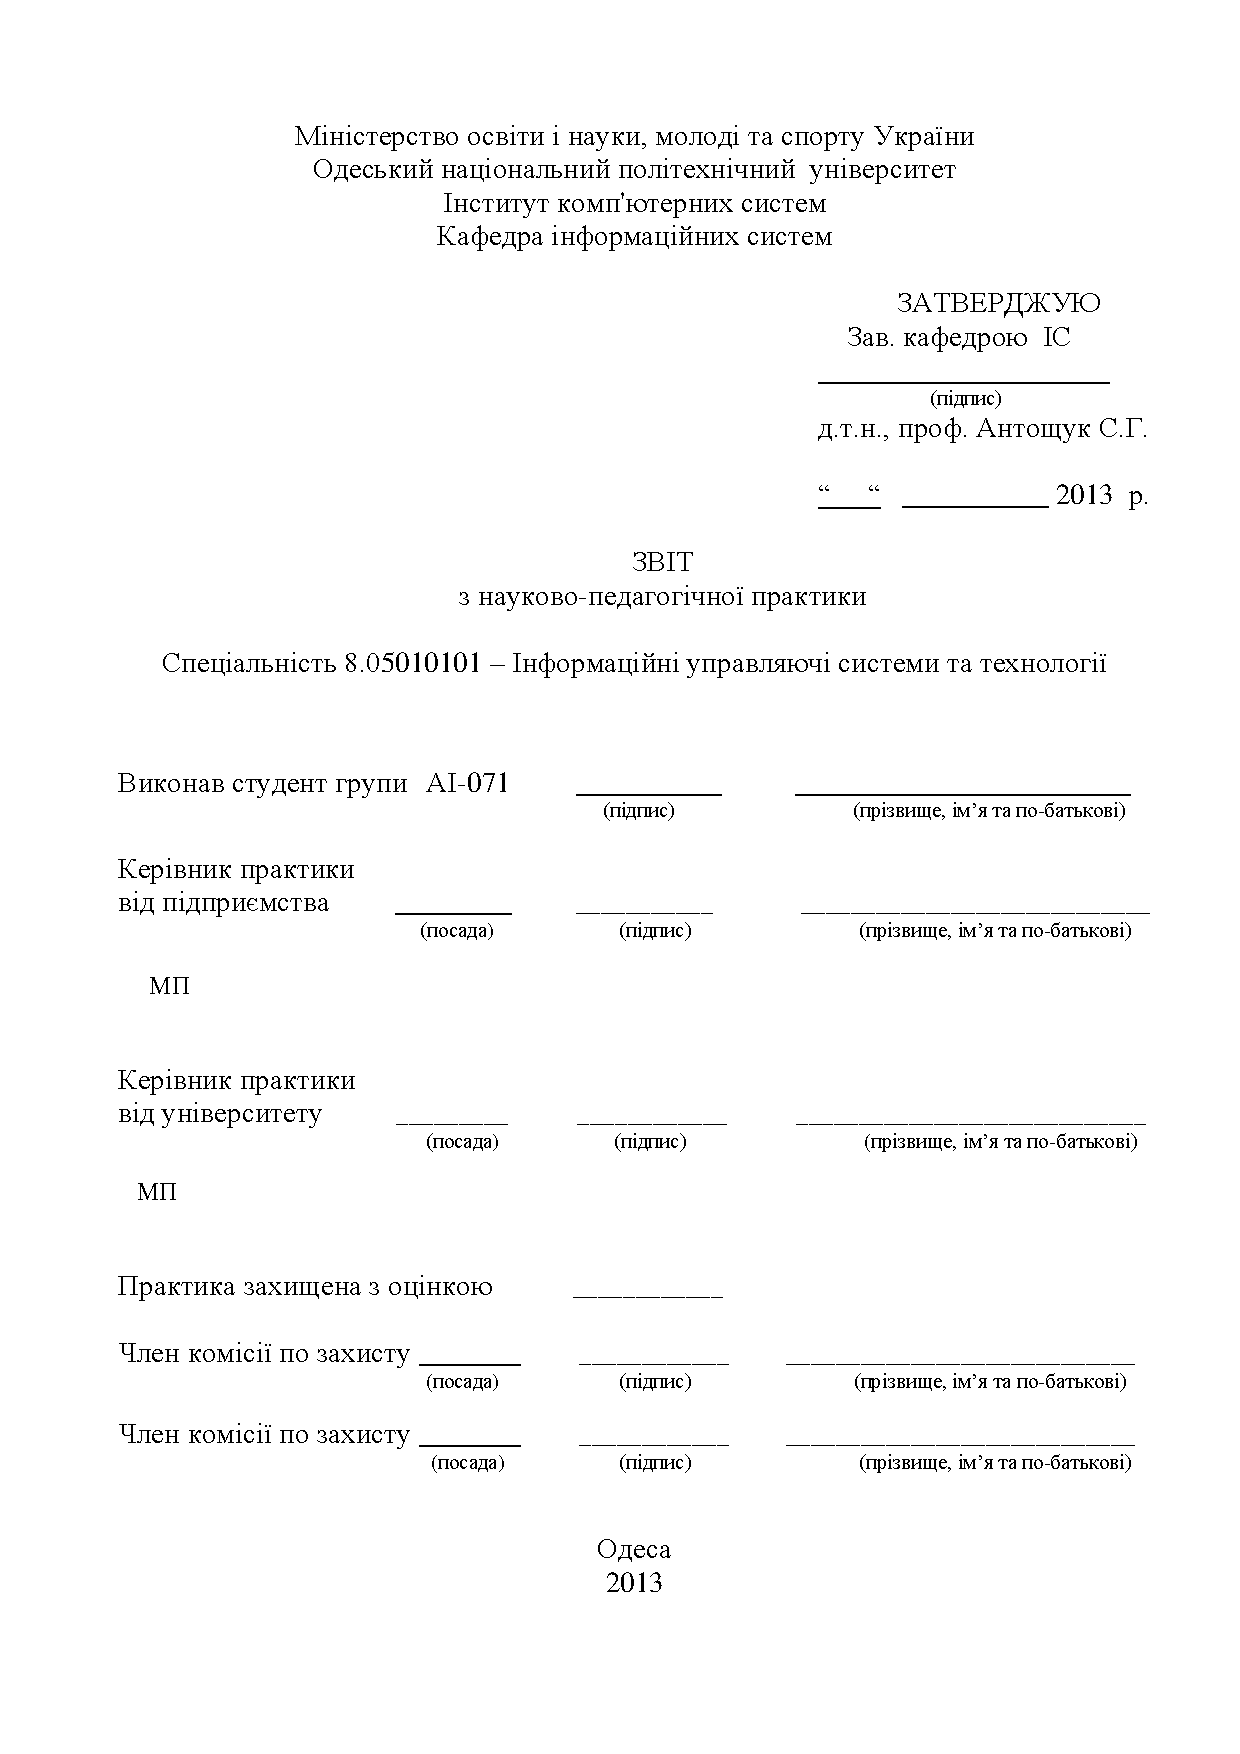
\includepdf[pages={1}]{titul/titul.pdf}

\ESKDthisStyle{formII}
% no page number on toc page: http://tex.stackexchange.com/a/2996/31897
\addtocontents{toc}{\protect\thispagestyle{empty}} 
\tableofcontents

% \newpage

\sectionnonum{Вступ}

% Індивідуальне завдання з практики відповідає темі дипломного проекту, яка  формулюється як «Дослідження та розробка протоколів бездротових мереж на основі стандарту \iee для управління елементами індикації медіа фасаду». Результати можуть бути далі використані в дипломному проекті. В результаті виконання індивідуального завдання з практики був проведений огляд існуючих методів аналогів в області дослідження, запропонована методика вирішення поставленої задачі, розроблена програма на базі обраного алгоритму, проведено порівняльний аналіз та тестування системи.

\section{Аналіз сучасного стану проблеми контроля елементів медіафасадів} % (fold)
\label{sec:1}

\subsection{Медіа фасади}

\todoi{
Історія, класифікація

adhoc медіа фасад, посилання на мою сттатю на idaacs

blinken lights

требования к мобильним вузлам и к кааналам связи
}

\subsection{Фізичні формати цифрового мисетецтва} % (fold)
\label{sub:digital_art_physical_formats}

Сфера інформаційних технологій розвиваєтья достатньо довго і накопила достатньо багато прикладів, які дозволяють говорити про новий напрям мистецтва - цифрове мистецтво. Інофрмаційні цифрові технології за своєю природою є нематеріальними, віртуальними. Але, новітні технології дозволяють цифровим митцям зблизити спостерігача-користувача із об’єктом мистецтва за допомогою створення фізичних втілень своїх робіт. 

У роботі \todo{ref Das vierte Format  Die Fassade als mediale Haut der Architektur} Sauter надає класифікацію видів втілень, що використовуються при створенні об’єктів цифрового мистецтва, які він називає фізичними форматами:

\begin{itemize}
	\item екрани програм;
	\item інтерактивні інсталляції;
	\item інтерактивні простори;
	\item інтерактивна архітектура.
\end{itemize}

Далі наведемо короткі пояснення перерахованих фізичних форматів.

Екрани програм дозволяють встановити одно чи двосторонній диалог між одним користувачем та програмою. Діалог встановлюється за допомогою широкопоширених приладів інтерфейсу користувача, таких як клавіатури, миши, сенсорні екрани. У якості програм на екрані використовуються веб-додатки, відеозаписи, ігри, тощо.

Під інтерактивними інсталляціями Sauter розуміє будь які медіа проєкти, що оформлені у вигляді об’єктів чи інсталляцій для висловлюівання певного змісту. У якості прикладу наводиться інтерактивний стул, що обладнаний чутливою поверхньою, який виводить деяку інформацію при контакті. Цей тип фізичного формату вже дозволяє організовати як діалог між об’єктом та одним користувачем, так і багатьма користувачами. Ті користувачі, що не бажають безпосередньо взаємодіяти із інсталляцією, можуть бути спостерігачами і, таким чином, також брати участь у процессі створення та отримання вражень. 

Інтерактивні простори - це подальший розвіток ідеї інтерактивних інсталляцій. Визначальна відміна полягає в вриішальному значенні інтерактивного простору та поведінки в інсталляції. У якості прикладу Sauter наводить кімнату із інтрактивними стінами та поверхнями, що мають медійне призначення та дозволяють реактивну зміну кімнати у відповідь до дій відвідувача. У своїй більшості, інтерактивні простори є багатокористувацькими оточеннями, що пропонують командні враження. Таким чином, ціль інтерактивних просторів - ініціювати взаємодію відвідувача як із інтерактивним змістом простору, так й із іншими відвідувачами.

Інтерактивна архітектура, згідно до Sauterа, на цей час, у своїй більшості через економічні причини, представлена медійним дизайном фасадів будівель. Таким чином, медіа фасади виконоють роль медійної мембрани між будівлею та міським простором. Зазвичай, медіа фасади використвують світло, проєкцювання зображень та LED-екрани. Але, також, існують приклади перших дінамічних фасадів та будівель.

\subsection{Технічни характеристики медіа фасадів та інших інтреактивних систем}

Сучасні технології надають інжинерам та дізайнерам великий вибір засобів для створеня інтерактивних систем і об’єктів мистецтва. Зазвичай, складно створити деяку систему класифікації таких систем, яка б дозволяла виключно віднести одну чи іншу інсталляцію до визначенного типу. Замість цього, у роботі \todo{ref media facades exhibition companion} Tscherteu та Leeb наводядь деяки найбільш важливі технічні характеристики систем візуалізації \todo{ref figure}. Робота, перш за все, спрямована на опис характеристик меді фасадів, що видом інтерактивної архітектри за класифікацією Sauter (підрозділ \ref{sub:digital_art_physical_formats}), але наведені зарактеристики мають відношення і до трьох інших фізичних форматів, запропонованих у роботі Sauter.

\todoi{схема}

Далі наведемо короткі пояснення до запропонованих на \todo{ref figure} технічних характеристик.

\begin{enumerate}
	\item технології відображення за \todo{ref} поділяються на активно випромінюючі та неактивно випромінюючі. До активно випромінюючих належать досить звичайні LED-екрани та точкові LED, галогенні лампи, флюоресцентні та фосфоресціентні технології. До неактивно випромінюючих належать механічно-кінетичні системи, що приводяться у рух за допомогою моторів, сжатого повітря, вітру; проєктивні; статичні. До проєктивних фасадів належать фасади, на які зображення проєктується як із зовни, так й ізнутри (наприклад, із середини кімнат на вікна);
	\item до властивостей зображення відносяться:
		\begin{itemize}
			\item роздільність зображення, що змінюється від проєкта до проєкту. Наприклад, медіа фасад Blinkenlights формував зображення розміром $18x8=144$ пікселів, а в медіа фасаді Grand Lisboa використувується більж ніж 11 міліон пікселей;
			\item шаг та розмір піксела - піксели можуть бути як малими та сгрупованими разом (наприклад, екран компьютера) та і великими і рознесеними у просторі на декілька метрів (наприклад, вікна будівлі як окремі пікселі у проеєкті Blinkenlights);
			\item відстань до спостерігача так саме може змінюватися у великому диапазоні від метра до сотень метрів. Зазвичай, відстань до користувача та розмір піксела взаємопов’язані, але не виключене, наприклад, і використання великих пікселів на близький відстані для досягнення певних візуальних ефектів;
			\item яскравість залежить від обраної технології візуалізації. Цільова яскравість залежить, у першу чергу, від умов викоритсання системи - у день при сонячному освітленні чи у ночі у темряві;
			\item кольорова спроможність - система може бути монохромною (є чи немає світла), виводити відтінки одного кольору (фактично, зміна яскравості) чи відтінки багатьох кольорів.
		\end{itemize}
	\item постійність значить тривалість використання системи у одномі місці. Постійні системи вбудовані в будівлю на весь строк використання. Непостійні системи встановлюються тимчасово, зазвичай для окремих подій, фестивалей, виставок (наприклад, Фестиваль вогнів у м. Берлін);
	\item часткова чи повна прозорість - досить важливий параметер щодо медіа фасадів. Непрозорі медіа фасади можуть, наприклад, перекривати вікна будівлі і заважати їх використанню;
	\item розмірність значить розміщення зображення на площині чи в просторі. Окремо виділяється випадок так званого 2,5D, у якому для формування зображення використовується декілька площин (наприклад, зображення сформовано на сторонах будівлі);
	\item стійкість і енергоспоживання особливо важливі у мобільних інтерактивних інсталляціях, але є також важливим питанням при розробці і постійних медіа фасадів, оскільки від енергоспоживання великої системи візуалізації залежить вартість використання та підтримки системи.
\end{enumerate}


\subsection{Огляд технологій бездротового звя’зку}

Протягом останніх 10-20 років була розроблена велика кількість різноманітних стандартів та технологій для систем, які потребують бездротового зв’зку. Оскільки, коло задач дуже широке і потреби систем відрізняються, розроблені стандарти часто вирішують різні задачі або пропонуютьрішення одних й тих самих задач різними методами. Розглянемо декілька доступних технологій і оцінемо їх придатність для використання в системі управління елементами індикації медіа фасаду. Огляд та порівняння підготовлено за матеріалами\todo{link}

% Comparaitive_Wireless_Standards.pdf
% Kniga-w01.pdf

Далі будуть наведені деякі відомості про доступні технології бездротового зв’язку.

\paragraph{Bluetooth та Bluetooth Low Energy} % (fold)
\label{par:bluetooth_bluetooth_low_energy}

Технологія Bluetooth використовується для обміну даними між Bluetooth-спроможними пристріями в персональних радіомережах. 

Технологія розробляється групою компаній Bluetooth Special Interest Group (Bluetooth SIG). З 2002 по 2005 діяла робоча група IEEE 802.15.1 по стандартизації технології, але на даний момент робота групи припинена і розробка спеціфікацій ведеться під контролем SIG.

Для зв’язку в технології Bluetooth використовується ISM диапазон радіочастот 2,4 ГГц, що дозволяє в деяких випадках встановлювати радіообмін на дистанціях більше ста метрів на відкритому простірі(пристрії класу 1). Однак, треба зауважити, що звичайні широко розповсюджені мобільні прилади, що використовують Bluetooth, здатні вести радіообмін лише на дистанціях 1-10 метрів (пристрії класів 2 та 3). Пропускна здібність змінювалась протягом версій стандарту. В версія 1 та 2 для передачі даних використовується лише канал зв’язку Bluetooth, специфікації версій 3 та 4 дозволяють комбіновану передачу даних із допомогою Wi-Fi. Найбільша пропускна здібність самого каналу Bluetooth досягнена в специфікації версії 2.1 і становлює 3 Мбіт/с.\todo{ref bt spec 2.1} 

Кожна мережа Bluetooth використовує 79 каналів. Bluetooth використовує технологію адаптивної зміни частоти (adaptive frequency hopping). Поточний канал постійно змінюється у визначеному порядку, що дозволяє знайти та уникнути діапазони радіохвиль, в яких присутній високий рівень зашумлення. Ця технологія, в першу чергу, направлена на забеспечення співіснування мереж Bluetooth із мережами Wi-Fi.

Група пристріїв в мережі Bluetooth зветься piconet. Мережа pcionet - це ad-hoc мережа. Один з пристроїв завжди є координатором мережі, наступні пристрої під’єднуються до мережі. При цьому, роль координатора може переходити від одного пристроя до іншого. Один координатор здатен підтримувати до 7 пристроїв в мережі (загально 8 пристріїв в мережі). Декілька pcionet-мереж можуть бути об’єднані в scatternet-мережу.

Bluetooth Low Energy (Bluetooth LE) - це частина спеціфікації Bluetooth, розробка якої була почата  компанією Nokia під назвою WiBree. В 2010 році Bluetooth LE став составною частиною нової, четвертої, версії основної спеціфікації. Bluetooth LE призначена скоротити потреби енергії і зменьшити вартість Bluetooth-рішень, зберігаючаи при цьому такуж дальність дії, як і у класичному Bluetooth. Пропускна спроможність Bluetooth LE, однак, меньша ніж у Bluetooth і сягає 1 Мбіт/с.

% paragraph bluetooth_bluetooth_low_energy (end)

\paragraph{Wi-Fi} % (fold)
\label{par:wi_fi}

Wi-Fi - це одна з найросповсюдженіших технлогій бездротового цифрового зв’язку. Wi-Fi призначена для поєднання різноманітних цифрових пристроїв у локальну мережу через бездротовий канал зв’язку. 

Розробка стандарту проводиться у робочій групі IEEE 802.11 за підтримкою організації Wi-Fi Alliance. Перша версія стандарту була опублікована у 1997 році. У подальшому, робочую групою було опубліковано декілька десятків виправлень та доповнень до базового стандарту і активна розробка продовжується.

Для зв’язку в технології Wi-Fi використовується ISM диапазон радіочастот 2,4 ГГц, а також в диапазоні 5 ГГц. Дальність зв’язку порізнюється залежно від використаних антен та характеристики оточуючого простіру. У загальному випадку, дальність може сягати 100 метрів на відкритому простірі і 35 метрів - у приміщені. Пропускна здібність неодноразово підвищувалась завдяки введенню нових стандартів. Стандарт IEEE~802.11g-2003 дозволяє досягти пропускної здібності 54 Мбіт/с, IEEE~802.11n-2009 - від 150 Мбіт/с до 600 Мбіт/с (найвища пропускна здібність при використанні 4 потоків передачі). 

Підтримувані мережою Wi-Fi канали залежать від робочого діапазону частот, ширіни каналу та правил у країні використання. У загальному випадку для мережі стандарту 802.11b/g/n, що працює у диапазоні 2,4 ГГц та використовує канали шириною 20 МГц, можливо 13 частково перекриваючихся каналів чи 4 неперекривающихся. 

\todoi{image channels}
% http://en.wikipedia.org/wiki/File:2.4_GHz_Wi-Fi_channels_%28802.11b,g_WLAN%29.svg

Група пристроїв в мережі Wi-Fi зветься \engtxt{Basic Service Set} (BSS). BSS бувають незалежні (\engtxt{Independent BSS}) чи інфраструктурні (\engtxt{Infrastructure BSS}). Незалежні BSS утворють ad-hoc мережу, в якій немає окремо зазначених точок доступу. Мережі, що працюють в інфраструктурному режимі, потребують окремо зазначену точку доступу, яка займається керуванням мережі. Декілька інфраструктурних BSS мереж можуть бути об’єднані в \engtxt{Extended Service Set} (ESS), шляхом об’єднання точок доступу окремих BSS через \engtxt{Distribution Network}. Використання ESS дозволяє, серед іншого, забеспечити роумінг пристріїв при переміщенні від одної BSS до іншої. Об’єднати незалежні BSS в ESS неможливо, оскільки в них немає точок доступу.

Кількість пристроїв залежить від режиму роботи мережі: в інфраструктурному режимі - 2007, в ad-hoc режимі - необмежено.

% paragraph wi_fi (end)

\paragraph{UWB} % (fold)
\label{par:uwb}

UWB - це набор стандартів бездротових персональних радіомереж із високою пропускною спроможністю - HR-WPAN (High Rate Wireless Private Area Network).

Розробка стандарту проводилася робочую групою IEEE~802.15.3 за підтримкою організацій UWB Forum та WiMedia Alliance. У 2003 році робочою групою був опублікований стандарт IEEE~802.15.3-2003 що описував MAC та PHY рівні для HR-WPAN. У подальшому в 2005 та 2009 роках були опубліковані доповнення до стандарту. У 2009-2010 роботи по розробці стандарту було припинено і дії організації WiMedia Alliance було припинено.

Для зв’язку в технології UWB використовуються диапазони радіочастот 3,168-10,560 ГГц (IEEE~802.15.3-2003)  та 57-66 ГГц (IEEE~802.15.3с-2009). Пропускна спроможність на відстанях до 10 метрів сягає від 110 Мбіт/с до 2 Гбіт/с для IEEE~802.15.3-2003 та від 1,54 до 5,75 Гбіт/с для IEEE~802.15.3с-2009.

\todo{ref ieee 802.14.3a moba approach}
\todo{ref IEEE 802.15.3c  The First IEEE Wireless Standard for Data Rates over 1 Gbps}

У публікаціях, що були видані протягом 2002-2009 років, висловлюються великі сподівання щодо UWB, оскільки стандарт забеспечує дуже високу пропускну спроможність та використовує діапазаони радіохвиль, що не використовуються в інших поширених технологія (Wi-Fi, тощо). Але, на цей час стандарт никим не підтримується і майбутнє стандарту не відомо.

% paragraph uwb (end)

\paragraph{\iee} % (fold)
\label{par:iee}

\iee - це стандарт для бездротових персональних радіомереж із низькою пропускною здібністю – LR-WPAN (\engtxt{Low Rate Wireless Private Area Network}). 

Розробка стандарту проводиться робочою групою \iee. Перша версія стандарту була опублікована в 2003 році. Остання ревізія стандарту була опублікована у 2011 році. 

Стандарт лежить в основі спеціфікацій технологій ZigBee, WirelessHART, MiWi, ISA100.11a. Підтримка \iee заявлена в спеціфікації 6LowPAN.\todo{links}

Для зв’язку в технології \iee використовується ISM диапазони радіочастот 868 МГц, 915 МГц та 2,4 ГГц. Декілька інших диапазонів лицензовані для використання у Японії та Китаї. Дальність роботи сягає 10-100 метрів і залежить від характеристик використаного радіопередавача. Пропускна здібність сягає 250 кбіт/с у диапазоні 2,4 ГГц. Кількість пристроїв в мережі обмежена використаним режимом адресації, нижня планка становлює 65530 пристроїв.

Окермо слід зауважити існівання додатку до стандарту IEEE 802.15.4a-2007, який додає підтримку нового PHY рівню на базі технології UWB. Згідно до цього додатку, номінальна пропускна здібність у диапазоні 2,4 ГГц становить 1 Мбіт/с, а в диапазонах UWB - від 851 Кбіт/с до 27,24 Мбіт/с.\todo{link to overview} Декілька компаній почали виробництво радіомодулів, що використовують додаток до стандарту.\todo{link to company}

% An Overview of the IEEE 802.15.4a Standard.pdf

% paragraph iee (end)

\todoi{інші технології?}

\subsection{Зведне порівняння технологій бездротового звя’зку}

В таблиці \ref{tbl:wireless_tech_comparison} наведено зведне порівняння основних розбіжностей технологій, що були оглянуті вище у підрозділах \labelcref{par:bluetooth_bluetooth_low_energy,par:wi_fi,par:uwb,par:iee}. Кожна технологія базується на стандарті IEEE\todo{інші технології?}. Wi-Fi та UWB забеспечують більшу пропускну спроможність, ніж Bluetooth та \iee. Wi-Fi призначений для встановлення бездротових локальних мереж. UWB, Bluetooth та \iee призначені діяти в WPAN-мережах.


\begin{table}[htbp]
\caption{Зведне порівняння оглянутих технологій бездротового зв’зку}
\hyphenpenalty=10000
\begin{tabular}{|p{0.18\textwidth}|p{0.175\textwidth}|p{0.175\textwidth}|p{0.175\textwidth}|p{0.175\textwidth}|}
\hline
                                       & Bluetooth               & Wi-Fi                                                  & UWB                     & IEEE 802.15.4            \\ \hline
Специфікація                           & IEEE 802.15.1 	         & IEEE 802.11g                                           & IEEE 802.15.3           & IEEE 802.15.4            \\ \hline
Частотний діапазон, ГГц                & 2,4                     & 2,4; 5                                                 & 3,168-10,56; 57-66      & 0,868; 0,915; 2,4        \\ \hline
Номінальна пропускна здібність, Мбіт/с & 1-3                     & 54-600                                                 & 110-5750                & 0,25                     \\ \hline
Дальність, м                           & 1-100                   & 35-100                                                 & 1-10                    & 10-100                   \\ \hline
Кількість каналів                      & 79                      & 14                                                     & 1-15                    & 27                       \\ \hline
Базова топологія мережі                & Piconet                 & BSS                                                    & Piconet                 & Зірка                    \\ \hline
Максимальна кількість вузлів           & 8                       & 2007                                                   & 8                       & Більш 65530              \\ \hline
Розширена топологія мережі             & Scatternet              & ESS                                                    & Peer to Peer            & Mesh, cluster tree       \\ \hline
Механізм співіснування                 & Адаптивна зміна частоти & Дінамічний вибір частоти, контроль потужності передачі & Адаптивна зміна частоти & Дінамічний вибір частоти \\ \hline

\end{tabular}

\label{tbl:wireless_tech_comparison}

\end{table}

\todoi{full diapasons}


\subsection{Висновки до розділу}

В цьому розділі були наведені відомості про системи медіа фасадів, були розгялнуті їх задачі і сценарії використання. 

Серед інших типів систем медіа фасадів був окремо виділений тип ad-hoc медіа фасадів. Системи цього типа характеризуються розподіленим виконання задач візуалізації та взаємодії із користувачем. Росподілені вузли для функціонування у рамках цілої системи повинні бути об’єднані в єдину мережу. Для забезпечення мобільності вузлів в цілях покращенної взаємодії з користувачем, полегшеного розгортання системи, тощо, було запропоновано використати бездротові радіомережі.

Через свої особливості, системою ad-hoc медіа фасаду виставляються наступні вимоги:\todo{}

Для виконання перерахованих вище вимог, були відібрані та оглянуті деякі технолгії бездротового радіозв’зку, а саме Bluetooth, Wi-Fi, UWB, \iee. Було проведено зведне порівняння відібраних технологій. За ітогами порівняння, пропонується використовувати технологію на базі стандарту \iee для побудови радіомережі у системі ad-hoc медіа фасаду. 


% section аналіз_сучасного_стану_проблеми_контроля_елементів_медіафасадів (end)

\section{Аналіз стандарту \iee}

В розділі~\ref{sec:1} для побудування радіомережі в системі ad-hoc медіа фасаду була вибрана технологія радіомереж на базі стандарту \iee. Для того, щоб можно було приступити до розробки протоколу прикладного рівня, необхідно розглянути можливості, що забеспечуються стандартом \iee.

У цьому розділі розглядається стандарт \iee, можливості що ним підтримуються та режими роботи, що можуть бути використані при розробці протоколу управління елементами індикації медіафасаду. 


\subsection{Стандарт \iee}
\label{sub:ieee:standard}


Стандарт \iee зосереджується на низько швидкісному, низько складному, енерго-ефективному бездротовому радіозв’язку серед пристроїв. Деякі з найбільш важливих особливостей стандарту, що можуть бути використані при розробці протоколу управління елементами індикації медіа фасаду, є:
\begin{itemize}
	\item підтримка мережевих топологій зірка та Peer-to-Peer;
	\item використання алгоритму CSMA-CA (\engtxt{Carrier Sense Multiple Access with Collision Avoidance} - множинний доступ з контролем несучої і униканням колізій);
	\item підтримка необов’язкового режиму доставки у реальному часі із використанням GTS (Guaranteed Time Slots – гарантованих  часових інтервалів);
	\item низькі вимоги до рівня споживання енергії;
	\item контроль споживання енергії за допомогою LQI (Link Quality Indication – показник якості зв’зку) та ED (Energy Detection – виявлення енергії).
\end{itemize}

Типово, пристрої \iee працюють в персональному просторі розміром 10 метрів чи менше. Але, робоча дальність залежить від обраного апаратного забезпечення і може досягати десятків та сотень метрів.\todoi{что конкретно говорит стандарт}

Сдантартом підримується декілька різних диапазонів радіочастот та форматів модуляції. Перша версія стандарту зазначала підтримку трьох диапазонів 2,4 ГГц, 915 МГц та 868 МГц із групи диапазонів ISM (Industrial, Scientifical and Medical radio bands – промислові, наукові та медичні діапазони радіочастот), який не підлягаю ліцензуванню у більшості країн. Подальші версії стандарту додали інші диапазони та методи модуляції. Повний список, згідно до поточного стандарту, наведено у таблиці\todoi{таблица из стандарта, страница 163}.

\todoi{freq bands and data rates}

Диапазони частот поділені на канали. Нумерація каналів проводитья із допомогою номерів каналів та страниць каналів. Диапазони, що були використані у першій версії стандарту віднесені до страниці каналів 0. До цієї страниці відносяться 27 каналів: 
\begin{itemize}
	\item 1 канал в диапазоні 868 МГц $(k = 0)$;
	\item 10 каналів в диапазоні 915 МГц $(k = 1, \cdots, 10)$;
	\item 16 каналів в диапазоні 2,4 ГГц $(k = 11, \cdots, 26)$.
\end{itemize}

\iee підтримує два типи пристроїв: FFD (Full-Function Device – повнофункціональний пристрій) та RFD (Reduced-Function Device – пристрій із зниженою функціональністю). RFD пристрої призначені для використання у дуже простих випадках і здібні асоціюватися лише із одним FFD. Це дозволяє втілити RFD пристрій при дуже обмеженому обсязі пам’яті, обчислювальної потужності та запасів енергії. Кожна мережа повинна містити як найменьш один FFD пристрій. 

Залежно від прикладної задачі, \iee мережа може мати топологію зірка чи Peer-to-Peer. 

Обидва типи мереж повинні мати один спеціальний пристрій – PAN координатор. PAN координатор створює мережу, дозволяє іншим пристроям асоціювати себе із мережею та контролює доступ пристроїв до мережі у випадку використання режиму роботи із маячками (beacon-enabled mode). Тільки FFD пристрій може стати PAN координатором.

Головна різниця між мережевими топологіями полягає у напрямках комунікації, що підтримуються. Мережа-зірка підтримує комунікацію лише між PAN координатором та асоційованим пристроєм. Peer-to-Peer мережа дозволяє довільні сполучення між усіма асоційованими пристроями.

Стандарт \iee визначає два режими роботи:
\begin{itemize}
	\item режим роботи без маячків (beacon-less mode) чи безслотовий (unslotted);
	\item режим роботи із маячками (beacon-enabled mode) чи слотовий (slotted).
\end{itemize}

Розуміння цих механізмів допоможе нам розробити мережеві протоколи.


\paragraph{Режим роботи без маячків}

CSMA – це алгоритм, який використовується для контролю часу передачі в мережі, яка складається із множини пристроїв (\figref{fig:csma-ca}).

\begin{figure}[bth]
	\centering
	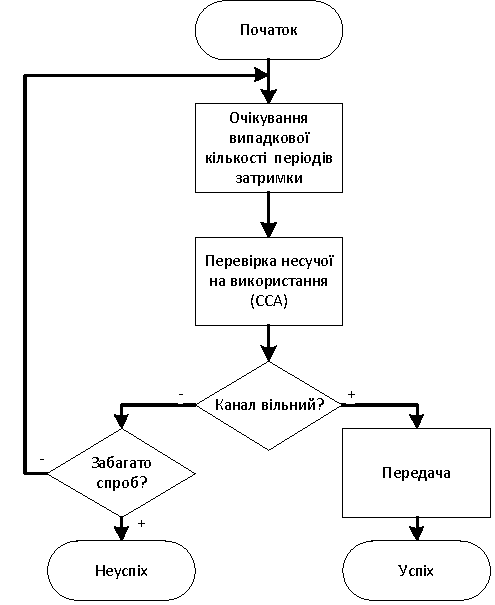
\includegraphics[width=0.7\textwidth]{img/csma-ca.pdf}
	% \missingfigure{csma-ca}
	\caption{\label{fig:csma-ca}Безслотовий алгоритм \csma, спрощена версія.}
\end{figure}

Пристрої використовують контроль несучої для того, щоб визначити період часу, коли канал «вільний» і протягом котрого можливо передати інформацію. Таким чином пристрій намагається уникнути колізії. Звісно, цілком можливий випадок, коли два пристрої вирішать почати передачу  одночасно протягом одного  «вільного» періоду. Для того, щоб зменшити ймовірність цього випадку, використовується механізм випадкових періодів затримки (random back-off delay) перед початком передачі. Випадкові затримки збільшують ймовірність успішного несумісного захвату каналу одним пристроєм.

У мережі, яка діє в режимі без маячків, усі пристрої використовують безслотовий алгоритм \csma. В загальному випадку, періоди затримки різних пристроїв не синхронізовані один з одним.  Кожен пристрій починає відраховувати випадковий період затримки і передачу за бажанням. Всі пристрої конкурують один з іншим за право використання каналу зв’язку. 

\clearpage

\paragraph{Режим роботи із маячками}
\label{par:beacon:enabled:mode}

\iee визначає додатковий, необов’язковий режим роботи із маячками. Під час цього режиму роботи, усі передачі виконуються в рамках суперкадрів (superframes). 

Кожен суперкадр складається із чотирьох частин (\figref{fig:superframe}):

\begin{itemize}
	\item маячок;
	\item CAP (Contention Access Period – період конкурентного доступу);
	\item Необов’язковий CFP (Contention Free Period – період без конкурентного доступу);
	\item Необов’язковий період неактивності.
\end{itemize}

\begin{figure}[bth]
	\centering
	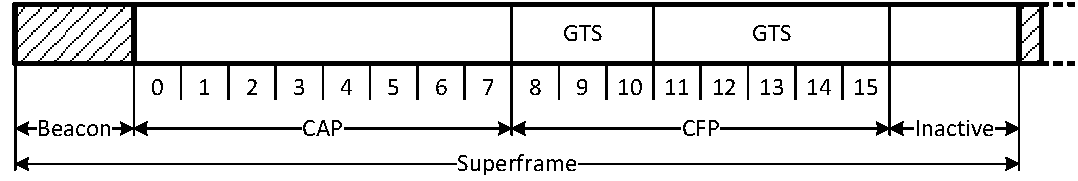
\includegraphics[width=\textwidth]{img/superframe.pdf}
	\caption{\label{fig:superframe}Схема суперкадру.}
\end{figure}

PAN координатор передає кадр-маячок на початку кожного суперкадру. Інші учасники мережі використовують отриманий маячок для того, щоб синхронізуватися із координатором. Також маячок використовується для доставки опису структури поточного суперкадру та іншої загальної інформації про мережу. 

Безпосередньо слідом за маячком починається період CAP. Протягом цього періоду усі асоційовані прилади в мережі використовують слотовий алгоритм \csma. Слотовий алгоритм \csma є модифікацією безслотового алгоритму. Пристрої так само конкурують за право передачі. Зміна полягає у наступному: якщо передача не може бути закінчена цілком до кінця періоду CAP, тоді вона взагалі не буде проведена протягом поточного періоду CAP. Замість того, вона буде відкладена до наступного. % Лише кадри підтверджень доставки та деяких інших спеціальних команд передаються без використання \csma.

Якщо PAN координатор вирішив на початку суперкадру, що  той повинен містити необов’язковий період CFP, тоді CFP починається після закінчення періоду CAP. Координатор поділяє період CFP на гарантовані часові інтервали (GTS). Якщо пристрій бажає передати інформацію протягом періоду CFP, він повинен отримати дозвіл на це від PAN координатора за допомогою службової команди GTS Request. Дозвіл від координатора отримується протягом періоду CAP. Якщо дозвіл отримано, пристрій має виключне право на використання призначеного йому інтервалу GTS. Таким чином, протягом інтервалу GTS алгоритм \csma не використовується. Але, звісно, пристрій зобов’язаний дотримуватися границь інтервалу GTS. 

Необов’язковий період неактивності може бути назначений PAN координатором для того, щоб пристрої могли перейти до сплячого енергозберігаючого режиму. Період неактивності починається після періоду CFP (чи CAP, якщо CFP у поточному суперкадрі відсутній) і завершується із завершенням поточного суперкадру.
Негайно із завершенням поточного суперкадру починається наступний суперкадр. 

\paragraph{Оцінка пропускної спроможності}
\label{par:throughput:evaluation}

Декілька досліджень було проведено для оцінки характеристик мереж на основі стандарту \iee, таких як максимальна пропускна спроможність, мінімальна та максимальна затримка доставки. Дослідники використовували різноманітні підходи: теоретичні розрахунки, експерименти за допомогою симуляції математичних моделей мереж чи за допомогою справжніх мереж.

Безслотовий алгоритм \csma та режим роботи без маячків у мережах стандарту \iee був досліджений у~\cite{thoroughput:analysis:unslotted:ieee}. Цій дослід стверджує, що режим роботи без маячків має меншій рівень накладних витрат, ніж режим роботи із маячками, і тому дозволяє досягти найбільшої пропускної спроможності. У досліді пропонуються аналітичні формули для оцінки значень пропускної спроможності та затримки доставки. Коректність запропонованих формул була перевірена експериментально.

Дослід~\cite{thoroughput:analysis:unslotted:ieee} пропонує оцінювати корисну пропускну здібність як функцію від розміру корисного навантаження кадру (\figref{fig:throughput_graph}). За допомогою розрахунків встановлено, що верхня межа корисної пропускної здібності в мережі, яка використовує 16 біт для адресування, сягає рівню 151 кбіт/с із відключеним механізмом підтверджень чи рівню 139 кбіт/с – із включеним. Із зменшенням розміру корисного навантаження кадру, корисна пропускна здібність також зменшується. Розмір заголовку кадру (і, відповідно, можливий розмір корисного навантаження) змінюється відповідно до обраного режиму адресування та параметрів безпеки. Тобто, максимальна корисна пропускна здібність залежить від обраних параметрів мережі.

\begin{figure}[bth]
	\centering
	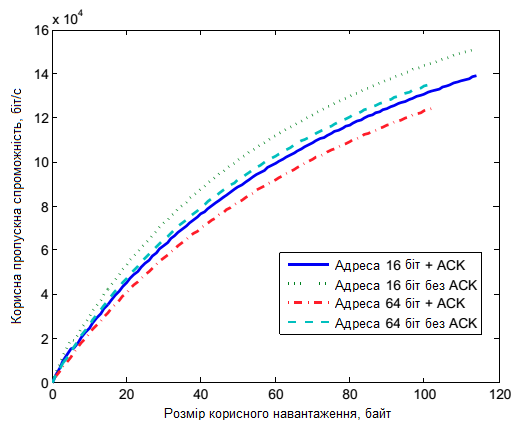
\includegraphics[width=0.7\textwidth]{img/throughput_graph.png}
	% \missingfigure{}
	\caption{\label{fig:throughput_graph}Корисна пропускна здібність як функція корисного навантаження, режиму адресування та настройок підтвердження доставки (ACK).}
\end{figure}

Експерименти, що були проведені у досліді~\cite{thoroughput:analysis:unslotted:ieee}, показують стабільну різницю між оціненою та експериментально виміряною корисною пропускною здібністю. Виміряна корисна пропускна здібність була десть на 11\% нижче за очиковану, тобто максимально досягнута пропускна здібність становила біля 123 кбіт/с.

Протягом практики мною були проведені власні експерименти по вимірюванню корисної пропускної здібності мереж \iee. Вимірювальні пристрої були побудовані на базі Arduino Leonardo та трансиверів MRF24J40MA. Експериментально виміряна корисна пропускна здібність встановила 110 кбіт/с. Цей результат добре відповідає результатам, що були отримані у~\cite{thoroughput:analysis:unslotted:ieee}.

Слотовий алгоритм \csma та режим роботи із маячками у мережах стандарту \iee був досліджений в ~\cite{simulation:study:slotted:ieee} та в ~\cite{gts:allocation:analysis}. Серед іншого, ці досліди встановлюють взаємозв'язок між порядком суперкадра (superframe order, розмір суперкадра) та максимальною пропускною здібністю. Досліди стверджують, що пропускна здібність сягає свого здійснимого максимуму, якщо порядок суперкадру дорівнює 3 або 4. При більших порядках, пропускна здібність зменшується.

Аналіз та порівняння слотового та безслотового алгоритмів \csma в стандарті \iee було проведено в ~\cite{analysis:slotted:unslotted}. У висновках досліду зазначається, що безслотовий алгоритм \csma  показує більшу максимальну пропускну здібність у порівнянні із слотовим алгоритмом \csma.

Але, цей висновок не є підставою для того, щоб вважати режим роботи із маячками, який використовує слотовий алгоритм \csma, повністю непотрібним. Цей режим пропонує дуже важливі особливості, які можуть бути використані для розробки мережевих протоколів специфічних для прикладної програми.

\section{Мережевий протокол для системи медіа фасаду}
\label{sec:network:protocol:amf}


Цей підрозділ присвячений розробці мережевого протоколу для системи медіа фасаду. Будуть проаналізовані архітектура та сценарії використання, запропоновані рішення щодо розроблюваного протоколу, а також буде розглянута окрема оптимізація протоколу.

\subsection{Архітектура системи}
\label{sub:system:arch}

Перед усім, розглянемо архітектуру системи ad-hoc медіа фасаду (\figref{fig:sys_arch}). 

\begin{figure}[bth]
\centering
\adjustbox{max width=\textwidth}{
	%!TEX root = ../praktika.tex


\begin{tikzpicture}[auto, node distance=6em,]

	\tikzstyle{block}=[draw, text width=5.7em, text centered, minimum height=3em, fill=white]

	\begin{pgfonlayer}{foreground}
		\node[block] (hc) {Хост-контролер};
		\node[block, below of=hc] (ha) {Хост-додаток};
		\node[block, right of=ha, node distance=10em] (ra) {Вiддалений додаток};
		\node[block, right of=hc, node distance=10em] (ln) {Вузел};

		\draw[thick,<->] (hc.south) -- (ha.north);
		\draw[thick,<->] (ha.east) -- (ra.west);
		\draw[thick,<->] (hc) -- (ln);

		\path (hc.west) -- (ln.east)
			 node[pos=0.5](betw-hc-ln) {} ;

		\node[block, above of=betw-hc-ln, text width=10em, node distance=4em] (sen) {Сенсори};

		\draw[thick,->] (sen) -- (hc);
		\draw[thick,->] (ln) -- (sen);
	\end{pgfonlayer}

	\begin{pgfonlayer}{background}
		\path (hc.west |- sen.north)+(-0.5,0.8) node (a) {};
		\path (ha.east |- ha.south)+(0.5,-0.3) node (b) {};
		\path[draw] (a) rectangle (b);
	
		\path (ln.west |- sen.north)+(-0.5,0.8) node (c) {};
		\path (ln.east |- ln.south)+(0.5,-0.3) node (d) {};
		\path[draw] (c) rectangle (d);
	\end{pgfonlayer}

	\begin{pgfonlayer}{foreground}
		\draw[] (a) node[anchor=north west] (host-label) {Хост};
		\path[draw] (host-label.south west) -- (host-label.south east) -- (host-label.north east);
		
		\draw[] (c) node[anchor=north west] (node-label) {Вузел};
		\path[draw] (node-label.south west) -- (node-label.south east) -- (node-label.north east);
	\end{pgfonlayer}

\end{tikzpicture}

}
\caption{\label{fig:sys_arch}Загальна архітектура системи}
\end{figure}

Система поділяється на дві основні частини: Хост та Вузли візуалізації.

Вузли візуалізації виконують, перед усім, фактичну роботу по візуалізації, а також дозволяють користувачам системи взаємодіяти із системою. Вузли можуть мати необов’язкові сенсори, які можуть використовуватися системою для визначення положення Вузлів та інших видів взаємодії із користувачами.

До складу Хоста входять Хост-контролер, Хост-додаток та сенсори. Сенсори на стороні Хоста використовуються для визначення положення Вузлів. Хост-додаток проводить загальне керування візуалізацією, системою. Хост-контролер використовує інформацію від сенсорів для того, щоб розподілити керівні команди від Хост-додатка на окремі завдання для Вузлів. Хост-контролер проводить оновлення візуалізації, посилаючи необхідні команди Вузлам через канал зв’язку.

Блок Віддалений додаток представляє на схемі будь яку іншу систему, яка під’єднана до системи медіа-фасаду, але не приймає активної участі в процесі візуалізації. Це може, наприклад, бути деякий інтерфейс користувача для адміністрування системи, Web-додаток, сусідня система візуалізації, тощо.

\subsection{Зв’язок архітектури системи та мережевого протоколу взаємодії}

Згідно із запропонованою в підрозділі~\ref{sub:system:arch} архітектурою системи, Вузли візуалізації не підтримують зв’язок один з одним заради цілей прикладної системи, візуалізації. Вузли спілкуються лише із Хост-контролером, щоб отримати оновлення візуалізації, повідомити інформацію з сенсорів. Однак, спілкування між Вузлами заради цілей управління мережею знаходиться поза рамками запропонованої архітектури і не забороняється.

\paragraph{Випадки трафіку}
\label{par:traffic:cases}

Виходячи із наведеної в пункті~\ref{sub:system:arch} архітектури системи, можна виділити два види мережевого трафіку в системі:
\begin{itemize}
	\item трафік від Хоста к Вузлам;
	\item трафік від Вузлів к Хосту.
\end{itemize}

Обидва види не однорідні і складаються с команд та даних різного роду, розміру та вимог до QoS (Quality of Service – якість обслуговування). QoS – це гарантії від мережі до прикладної програми щодо якості характеристик каналу зв’язку: пропускна здібність, час доставки.

Трафік від Хоста к Вузлам складається, перед усім, з команд оновлення візуалізації. Ці команди змінюють візуальний стан Вузлів. Залежно від типу, природи візуалізації, до цього виду трафіка можуть пред’являтися різні вимоги щодо часу і гарантій доставки. Але, можна очікувати, що команди візуалізації будуть складати основну частину всього мережевого трафіку.

Одним з найпростіших для виконання механізмів оновлення візуалізаціє є наступний: усі Вузли оновлюються часто і одночасно, так само, як окремі пікселі на моніторі оновлюються одночасно при зміні кадру. При цьому механізмі, команди на оновлення відсилаються часто. В такому випадку, витрата однієї команди на оновлення буде менш помітна і менш впливова на загальний опит користувача. Більш важливою є доставка  команд оновлення у встановлені рамки ніж надійна доставка. Якщо команда запізнюється із доставкою – її все одно можна відкидати, бо вона застаріла і скоро прийде наступна. Цей підхід використовується в існуючих протоколах потокової передачі медіа-контенту. Звісно, якщо кількість відкинутих чи втрачених пакетів завелика, тоді якість сигналу падає аж до рівню повної непридатності. Таким чином, рівень допустимої кількості втрат залежить від конкретної прикладної задачі.

Крім команд оновлення візуалізації, трафік від Хоста к Вузлам може також містити інші види керуючих команд. Наприклад, Хост може використовувати модель Запит-Відповідь для отримання інформації з Вузлів: інформація з сенсорів на Вузлах, стан батареї, тощо. Можна очікувати, що цей тип трафіку має менші вимоги до QoS.

Основною складовою трафіку від Вузлів к Хосту є відповіді Вузлів на запити Хоста чи дані від сенсорів на Вузлах. Цей вид трафіку буде сягати значної долі у загальному мережевому трафіці у випадку, якщо використовується модель Запит-Відповідь, чи якщо сенсори на Вузлах створюсь багато інформації, яка часто відсилається до Хоста.

Обидва види трафіка також використовуються для підтримки мережі: створення мережі, асоціювання та де асоціювання пристроїв, синхронізація, маршрутизація, тощо.

\paragraph{Мережева топологія}

Вибір мережевої топології завжди залежить від поставленої прикладної задачі. Походячи із описаних в пункті~\ref{par:traffic:cases} видів трафіку, найбільш простою для використання буде топологія зірка. Згідно до архітектури системи (пункт~\ref{sub:system:arch}), Вузли спілкуються лише із Хостом, який, в такому випадку, є PAN координатором мережі.

Використання інших мережевих топологій можливо. Але підвищення складності може негативно позначитися на QoS характеристиках мережі.

\paragraph{Сценарії роботи мережевого протоколу}
\label{par:network:protocol:scenarios}

В пункті~\ref{par:traffic:cases} був наведений опис двох можливих видів трафіку. В цьому пункті ми розглянемо два різні сценарії можливих рівнів трафіку і запропонуємо варіації мережевого протоколу для них.

Як вже зазначалося вище, ми очікуємо витрачати основну частину пропускної здібності мережі на оновлення візуалізації, тобто на трафік від Хоста к Вузлам. Припустимо, що це очікування вірне. Тоді, маємо два можливі сценарії рівня трафіку від Вузлів к Хосту:
\begin{itemize}
	\item незначний чи відсутній трафік;
	\item значний трафік.
\end{itemize}


\paragraph{Незначний чи відсутній трафік від Вузлів к Хосту}
\label{par:low:nthn}

Цей сценарій має місце у випадку, коли Вузли візуалізації не обладнані сенсорами чи сенсори оновлюють свої показники не часто. Керівні команди так саме невеликі і рідкісні. Це можливе у випадку, коли не використовується модель Запит-Відповідь та коли склад мережі змінюється не часто.

Для цього сценарію я пропоную використати режим роботи мережі без маячків. Кожен пристрій в мережі може почати передачу в будь коли, всі пристрої конкурують за доступ до каналу зв’язку. 

Як було зазначене вище у пункті~\ref{par:throughput:evaluation}, режим роботи без маячків дозволяє досягти найбільшої пропускної здібності мережі. Пуск, настройка та керування мережею простіші за режим роботи із маячками. Трафік від Хоста к Вузлам займає основну частину усього трафіку, тому можна очікувати, що конкурентні конфлікти доступу до каналу зв’язку будуть рідкісні і не впливові.

З іншого боку, якщо попередня оцінка рівню трафіка від Вузлів к Хосту не вірна і, насправді, рівень набагато вище, тоді пропускна здібність мережі буде зменшена через конкурентні конфлікти доступу. Таким чином, в приведеному сценарії є дуже важливою правильна попередня оцінка умов роботи системи.

Другий недолік запропонованого рішення полягає в процедурі асоціації приладів при підключенні до мережі. Асоціація при режимі роботи без маячків наступна: пристрій, що хоче приєднатися до мережі, відсилає команди Beacon Request (запит маячка) на кожній з доступних частот і очікує відповіді від PAN контролера. PAN контролер, отримавши  у свою чергу Beacon Request, вирішує, чи дозволити пристрою приєднатися до мережі і відповідає на запит. Як можна бачити, пристрої повинні активно розшукувати мережу, до якої можна приєднатися. Процедура активної асоціації пристроїв збільшує трафік від Вузлів к Хосту і, через це, зменшує QoS в мережі. Якщо склад мережі змінюється часто, нові Вузли будуть проводити активну асоціацію і негативно впливати на роботу мережі.

\paragraph{Значний трафік від Вузлів к Хосту}
\label{par:low:ntht}

Цей сценарій має місце у випадку, коли Вузли візуалізації обладнані сенсорами, які часто  оновлюють свої показники, або коли склад мережі змінюється часто.

Для цього сценарію я пропоную використати режим роботи мережі із маячками та GTS.

Як було зазначене вище у пункті~\ref{par:beacon:enabled:mode}, режим роботи із маячками дозволяє поділити суперкадр на два періоди: CAP та CFP. Я пропоную відвести основну долю суперкадру під CFP, протягом якого Хост відправлятиме команди оновлення візуалізації та іншу критичну інформацію. Залишок суперкадру відводиться під період CAP, протягом якого діють і Хост, і Вузли. CAP відводиться для некритичного трафіку в обидві сторони, доступ до каналу зв’язку проводиться на конкурентній основі. 

Виключне використання періоду CFP Хостом дозволяє ввести гарантії на QoS мережі, планувати пропускну спроможність та часи затримок. 

Процедура асоціації нових Вузлів також дещо простіша. Оскільки в мережі постійно на початку кожного суперкадру відправляються маячки із інформацією про мережу, новий Вузол може не проводити активну асоціацію. Замісць цього, він повинен пасивно прослуховувати кожну з доступних радіочастот, щоб отримати маячок на початку суперкадра. Отримавши маячок, новий Вузол може почати спілкування із Хостом протягам періоду CAP. Така пасивна асоціація забезпечує непереривання передачі важливого трафіка.

Режим роботи із маячками може бути додатково використаний для синхронізації часу між Вузлами та Хостом. Така часова синхронізація може буде використана в деяких стратегіях оновлення візуалізації.

До недоліків запропонованого режиму належить, перш за усе, необхідність додаткового налаштування параметрів суперкадру. Як було показано в пункті \ref{par:throughput:evaluation}, при зменшенні розміру кадру, зменшується пропускна здібність. Але, можна очікувати, що трафік від Вузлів до Хоста складатиметься саме із невеличких кадрів. Враховуючи велику кількість Вузлів в мережі, а також те, що частина суперкадру відведена під CFP, ймовірність колізій під час CAP тільки збільшується, а пропускна здібність падає. Тобто, система повинна бути готовою до затримок чи втрат доставки трафіку від Вузлів к Хосту. 

Відношення між розмірами CFP та CAP в такому випадку є найбільш впливовим параметром для регулювання якості та надійності доставки. Це рішення є компромісним.

\paragraph{Мультиплексування оновлення візуалізації}

У пункті \ref{par:traffic:cases} був розглянутий один з можливих механізмів оновлення візуалізації, при якому усі Вузли оновлюються разом і часто. При цьому механізмі, команди оновлення візуалізації  потрібно відправляти Вузлам на кожному «візуальному кадрі», тобто об’єм даних, що необхідно передати, є стабільно великим. «Наївна» реалізація використовуватиме відправлення окремих мережевих кадрів окремим вузлам.

Максимальний розмір кадру згідно до стандарту \iee становить 127 байт ~\cite{ieee:802:15:4:2011}. Деяку долю кадру займає MAC заголовок і контрольні поля. Як вже згадувалося в пункті \ref{par:throughput:evaluation}, заголовок має змінний розмір, який залежить від використаного режиму адресування та параметрів безпеки. У випадку, якщо ні поля безпеки, ні поля адресування не зазначені у заголовці, тоді розмір корисного навантаження кадру сягаю свого максимуму в 122 байти. Але, корисність протоколів, що зовсім не застосують адресування, обмежена, тому розмір корисного навантаження в 114-120 байтів є більш реалістичним. Невикористання повністю доступного простору для корисного навантаження призводить до погіршення пропускної здібності.

Розглянемо випадок, коли розмір окремої команди оновлення візуалізацію менший за максимальний розмір корисного навантаження кадра і, наприклад, становить 10 байт. Це припущення вірне у випадку, коли Вузол візуалізації обладнаний простими засобами і є аналогом лише декількох пікселей. Якщо в такій системі буде використаний механізм оновлення візуалізації, зазначений на початку пункту, із «наївною» реалізацією, яка потребує відправки окремих команд окремим Вузлам, тоді більшість кадрів будуть замалими для досягнення великої пропускної здібності.

Команди оновлення візуалізації для окремих Вузлів можна об’єднати разом і відправити одним мережевим кадром, тобто, команди можна мультиплексувати. Цей підхід дозволяє більш ефективно використати доступний простір під корисне навантаження і досягти більшої пропускної здібності. Такі мультиплексовані команди повинні бути відправлені до Вузлів за допомогою широкомовного кадру.

Мультиплексування може бути використане для обох сценаріїв, які були описані в пункті \ref{par:network:protocol:scenarios}.

\section{Симуляція}

\subsection{Огляд симуляторів мереж}

Існує декілька симуляторів для комп'ютерних мереж. Надалі роглянемо варіанти и обремо один для використання.

\paragraph{ns}
\label{par:ns}

ns - це симулятор мереж із дискритним часом подій, призначений для моделювання систем Інтернету із дослідницькою та навчальною ціллю. Симулятор росповсюджується під свободною ліцензією GNU GPLv2 і відкрито доступен для використання.

Актуальними на цей час є версії 2 та 3. 

Розробка версії 2 почалась у 1996 році, остання стабільна версія 2.35 була випущена у листопаді 2011 року. Розробниками була заявлена ціль випустити версію 2.36 наприкінці 2013 року\todo{ссилка http://nsnam.isi.edu/nsnam/index.php/Roadmap}. Нова версія призначена виправити деякі помилки, змінити скрипти для зборки, добавити декілька нових моделей. Але, взагалі розробка проєкт вважається основними розробниками закінченим.

Розробка версії 3 почалась у 2008 році. Розробники повністю відкинули старий кд і почали розробку з початку. Через те, не весь функціонал, що був підтриманий версією 2, присутній у версії 3. Версія зараз активно розроблюється. Остання версія 3.18 була опублікована у серпні 2013 року, наступна версія 3.19 запланована на грудень 2013\todo{link}.  
% http://www.nsnam.org/wiki/index.php?title=Current_Development&oldid=8062

ns-3 має початкову підтримку мереж стандарту \iee. Серед найбільших недоліків є підтримка MAC рівнем лише безслотового \csma і, через те, лише режиму роботи без маячків. Опис стану підтримки мереж стандарту \iee симулятором може бути знайдений в розробітницькій  документації в репозитрії сирцевого коду\todo{ссілка, поточний стан lr-wpan в ns3 http://code.nsnam.org/tomh/ns-3-lr-wpan/file/60fda85f5921/src/lr-wpan/doc/lr-wpan.rst}.

ns-2 має кращу підтримку мереж стандарту \iee. Повністю підтримується режим роботи без маячків. В режимі роботи із маячками підтримується передача даних у періоді CAP. Стандартна версія бракує підтримки GTS. Але у 2011 році підтримка GTS була розроблена у рамках досліду\todo{link Implementation of the IEEE 802.15.4 module with CFP in NS-2}.

\paragraph{OMNeT++}

OMNeT++ - це компонентний фреймворк для побудування симуляторів мереж. Сам по собі, OMNeT++ надає лише інструменти та інфраструктуру для побудування симуляцій. Моделі мереж росповсюджуються у складі інших фреймворків та бібліотек. 

\subsection{Модель мережі \iee у ns-2}

\paragraph{Загальна модель бездротової мережі}

Основним елементом моделі бездротової мережі у симуляторі ns-2 є MobileNode. 

Клас MobileNode походить від класу Node. Але, на відміну від звичайних Node у ns-2, об’єкти класу MobileNode не зв’язані один з іншим через об’єкти класу Link. Замість цього, ns-2 симулює передчу та прийом сигналів через радіоканал.

Клас MobileNode - розділений клас. Він агрегує у собі окремі компоненти, що дозволяє використовувати загальну схему MobileNode для моделювання різних технологій та алгоритмів. 

Загальна схема MobileNode зображена на \todo{ref}.

\todoi{img загальна схема mobile node}

Мережевий стек мобільного вузла складається із рівня зв’язку (LL), модуля ARP, очереді інтерфейсу (IFq), рівню MAC, мережевого інтерфейсу (netIF). Мережевий інтерфейс підєднується до каналу (Channel), який використовується усьома мобільними вузлами, за допомогою антени.

Надалі наведений опис класів, що входять до составу MobileNode:

\begin{itemize}
	\item Рівень LL відповідає за симуляцію протоколів канального рівню. Основною задачею LL є правильна установка MAC-адресу призначення у MAC-заголовці пакету. Для цього, LL підєднаний до компоненту ARP, який вирішує, який MAC-адрес відповідає зазначеному адресу вищого рівня (зазвичай, IP-адрес). Зазвичай, LL отримує всі вихідні (ті, що відправляються до каналу зв’язку) пакети від агента маршрутизації. Такі пакети LL відправляє до очереді інтерфейсу. Всі вхідні пакети (ті, отримані із каналу зв’язку) LL отримує від MAC.

	\item Компонент ARP (Address Resolution Protocol, протокол визначеня адрес) отримує запроси від LL. Якщо MAC-адрес вузла призначення відомий ARP, тоді цей адрес записується до MAC-заголовку пакета. Інакше, ARP за допомогою широкомовного пакету запрошує розшукуваний MAC-адрес у других вузлів і тимчасово приховує пакет, що відправляється, у кеші. Для кожного невідомого MAC-адресу, ARP тримає у кеші лише один пакет. Якщо поступає два пакети, старіший з них відкидаєтсья. Як тільки MAC-адрес вузла призначення стає відомим, пакет, що був прихований в кеші, повертається до LL і той передає пакет до очереді інтерфейсу.

	\item Очередь інтерфейсу - це очередь, що надає приоритет пакетам які відправлені протоколами роутінгу, вставляючи їх до початку очереді перед звичайними пакетами.

	\item Рівень MAC забезпечує коректне спільне використання загального середовища декількома вузлами мережі. 

	\item Мережевий інтерфейс виконує роль фізичного інтерфейсу, який використається мобільним вузлом для доступу до каналу зв’язку. Мережевий інтерфейс для бездротового радіозв’язку виконано як клас Phy/WirelessPhy та його дітей. Цей інтерфейс симулює передачу даних із підтримкою вказаної моделі розповсюдження сигналів. Також, підтримується обробка колізій передачі. При передачі, мережевий інтерфейс штампує фрейм і додає свої метадані (потужність випромінювання, частота радіохвиль, тощо). Метадані використовуються молеллю розповсюдження сигналів на приймаючій стороні для визначення, чи достатня потужність сигналу для детектування чи прийома пакету.

	\item Компонент модель розповсюдження сигналів використовує комбіновану математичну модель: на коротких відстанях використовується формула Фрііса (потужність прийнятого сигналу пропорційна $\frac{1}{R^2}$, де $R$ - відстань між антенами), а на великих відстанях використовується апроксимована двухпроменева модель розповсюдження сигналу ((потужність прийнятого сигналу пропорційна $\frac{1}{R^4}$). Апрокамація припускає відображення сигналу від плоскої поверхні. 

	\item У якості антени використовується об’єкт класу Antenna/OmniAntenna, що моделює всенаправлену антену із одинчним коефіцієнтом підсилення. 
\end{itemize}

\paragraph{Модель для симуляції \iee}

В таблиці \ref{tbl:simulation_classes} наведені класи компонентів що буди використані у симуляції бездротової мережі \iee.

\begin{table}[htbp]
\caption{Класи компонентів, що були використані для симуляції}
\hyphenpenalty=10000
% \begin{tabular}{|p{0.18\textwidth}|p{0.175\textwidth}}
\centering
\begin{tabular}{|l|l|}
\hline
Компонент                     & Клас                       \\ \hline
Канал зв’язку                 & Channel/WirelessChannel    \\ \hline
Антена                        & Antenna/OmniAntenna        \\ \hline
Мережевий інтерфейс           & Phy/WirelessPhy/802\_15\_4 \\ \hline
Модель розповсюдження сигналу & Propagation/TwoRayGround   \\ \hline
Рівень MAC                    & Mac/802\_15\_4             \\ \hline
Очередь інтерфейсу            & Queue/DropTail/PriQueue    \\ \hline
Рівень LL                     & LL/LL802\_15\_4            \\ \hline
Агент маршрутизації           & NOAH                       \\ \hline
\end{tabular}
\label{tbl:simulation_classes}
\end{table}

Симулятор ns-2 у стандартній комплектації не підтримує у необхідному обсязі всі неохідні для симуляції розробленого протоколу можлиівості стандарту \iee. Через те, до симулятору було внесено ряд змін:

\begin{enumerate}
	\item добавлено агент маршрутизації NOAH\todo{ref to noah}. ns-2 надає декілька реализацій алгоритмів для ad-hoc маршрутизації. На відміни від них, NOAH (No Ad-Hoc routing agent) використовує заздалегіть визначену статичну таблицю маршрутизації. Під час роботи не робить спроб обновити таблицю маршрутизації і не відправляє жодних службових пакетів. Використання NOAH дозволяє симулювати статичні мережі із заздалегіть відомою топологією.
	% http://icapeople.epfl.ch/widmer/uwb/ns-2/noah/

	\item NOAH змінено так, що алгоритм не змінює розмір пакету, що відправляється. Попередня поведінка - NOAH додавав до розміру пакету розмір IP-заголовку. 

	\item добавлено агент для генерації широкомовного трафіку. Імплементацію агента отримано за посиланням \todo{ref link}. Ця імплементація дозволяє генерировати CBR (constant bit-rate) широкомовний трафік на відміну від зазвичай використованих агента UDP та генератора CBR-трафіку. Використана імплементація широкомовного агента виправлена для того, щоб більш підходити до умов симуляції.
	% http://www.math.unipd.it/~cpalazzi/fastbroadcast.html

	\item добавлено клас LL/LL802\_15\_4, якій не використовує таблицю ARP. Замість цього, він використовує адрес із заголовку пакета як MAC-адрес. Також він дозволяє встановити флаг GTS для всіх вихідних пакетів. Клас Mac/802\_15\_4 використовує цей флаг для того, щоб обрати, коли відправляти пакет. 

	\item добавлена імплементація передачі даних протягом CFP у періодах GTS. Використована імплементація була розролена у рамках досліду \todo{link Implementation of the IEEE 802.15.4 module with CFP in NS-2} і була отримана за посиланням \todo{link}.

	\item до імплементації стеку 802.15.4 добавлена можливість вказати параметри GTS командою до PAN-координатора із скрипта симуляції. До цього, реалізація підтримувала тільки аллокацію періодів GTS по запиту від кінцевого вузла. Також, клас Mac/802\_15\_4 було змінено так, що PAN-координатор не забуває параметри виділених періодів GTS у наступному суперкадрі.

	\item виправлено деякі помилки в реалізації GTS, а саме:
	\begin{itemize}
		\item виправлена помилка яка блокувала можливість виділити період GTS тривалістю більше одного слота;
		\item виправлений помилка у розрахунку можливості виділення нового періоду GTS. Тепер під час розрахунку правильно враховується константа aMinCAPLenght, що дозволяє відводити під період CFP більшу часть суперкадра;
		\item виправлений ряд помилок, що не виключали можливість відправки пакетів PAN-координатором під час GTS;
		\item виправлена помилка у розрахунку тривалості передачі GTS, що призводила до помилкових відкидань повністтю прийнятих пакетів;
		\item виправлена помилка у розрахунку розміру заголовка пакету, що був оставлений для очікування наступного періоду GTS.
	\end{itemize}

\end{enumerate}

\subsection{Симуляція}

У цьому підрозділі проведемо симуляцію декількох випадків використання мережі. 

\paragraph{Перевірка швидкості}

Перша симуляція служитиме для встановлення верхньої границі пропускної здібності. Оцінка пропускної здібності вже була наведена в пункті \ref{par:throughput:evaluation}, де були використовані результати інших робіт. У цьому пункті буде первірено правильність наведених раніше оцінок та правильність роботи моделі мережі \iee.

Було перевірено декілька режимів роботи:

\begin{enumerate}
	\item режим роботи без маячків. Параметри симуляції вказані в таблиці \ref{tbl:simulation_settings_nonbeackon}.

	\begin{table}[htbp]
	\caption{Параметри симуяції режиму роботи без маячків}
	\hyphenpenalty=10000
	% \begin{tabular}{|p{0.18\textwidth}|p{0.175\textwidth}}
	\centering
	\begin{tabular}{|l|l|}
		\hline
		Параметер                     &                         \\ \hline
		Кількість вузлів              & 2                       \\ \hline
		Час симуляції, с              & 60                      \\ \hline
		Розмір корисного навантаження & 1..120                  \\ \hline
		Режим режим адресування       & 16 біт                  \\ \hline
		Режим підтвердження           & Із та без підтвердження \\ \hline
		Режим роботи                  & Без маячків             \\ \hline
	\end{tabular}
	\label{tbl:simulation_settings_nonbeackon}
	\end{table}

	Результати симуляції наведено на рисунках \ref{fig:result_tp_nonbeacon} та \ref{fig:result_jts_nonbeacon}.

	\begin{figure}[bth]
		\centering
		\adjustbox{max width=\textwidth}{
			% \input{/home/pashkoff/code/ns/my/test_speed_nonbeac/tp.pgf}
			%% Creator: Matplotlib, PGF backend
%%
%% To include the figure in your LaTeX document, write
%%   \input{<filename>.pgf}
%%
%% Make sure the required packages are loaded in your preamble
%%   \usepackage{pgf}
%%
%% Figures using additional raster images can only be included by \input if
%% they are in the same directory as the main LaTeX file. For loading figures
%% from other directories you can use the `import` package
%%   \usepackage{import}
%% and then include the figures with
%%   \import{<path to file>}{<filename>.pgf}
%%
%% Matplotlib used the following preamble
%%   \usepackage[utf8]{inputenc}
%%   \usepackage[T2A]{fontenc}
%%   \usepackage{pscyr}
%%
\begingroup%
\makeatletter%
\begin{pgfpicture}%
\pgfpathrectangle{\pgfpointorigin}{\pgfqpoint{6.000000in}{4.000000in}}%
\pgfusepath{use as bounding box}%
\begin{pgfscope}%
\pgfsetbuttcap%
\pgfsetroundjoin%
\definecolor{currentfill}{rgb}{1.000000,1.000000,1.000000}%
\pgfsetfillcolor{currentfill}%
\pgfsetlinewidth{0.000000pt}%
\definecolor{currentstroke}{rgb}{1.000000,1.000000,1.000000}%
\pgfsetstrokecolor{currentstroke}%
\pgfsetdash{}{0pt}%
\pgfpathmoveto{\pgfqpoint{0.000000in}{0.000000in}}%
\pgfpathlineto{\pgfqpoint{6.000000in}{0.000000in}}%
\pgfpathlineto{\pgfqpoint{6.000000in}{4.000000in}}%
\pgfpathlineto{\pgfqpoint{0.000000in}{4.000000in}}%
\pgfpathclose%
\pgfusepath{fill}%
\end{pgfscope}%
\begin{pgfscope}%
\pgfsetbuttcap%
\pgfsetroundjoin%
\definecolor{currentfill}{rgb}{1.000000,1.000000,1.000000}%
\pgfsetfillcolor{currentfill}%
\pgfsetlinewidth{0.000000pt}%
\definecolor{currentstroke}{rgb}{0.000000,0.000000,0.000000}%
\pgfsetstrokecolor{currentstroke}%
\pgfsetstrokeopacity{0.000000}%
\pgfsetdash{}{0pt}%
\pgfpathmoveto{\pgfqpoint{0.725417in}{0.625833in}}%
\pgfpathlineto{\pgfqpoint{5.690000in}{0.625833in}}%
\pgfpathlineto{\pgfqpoint{5.690000in}{3.739792in}}%
\pgfpathlineto{\pgfqpoint{0.725417in}{3.739792in}}%
\pgfpathclose%
\pgfusepath{fill}%
\end{pgfscope}%
\begin{pgfscope}%
\pgfpathrectangle{\pgfqpoint{0.725417in}{0.625833in}}{\pgfqpoint{4.964583in}{3.113959in}} %
\pgfusepath{clip}%
\pgfsetrectcap%
\pgfsetroundjoin%
\pgfsetlinewidth{1.003750pt}%
\definecolor{currentstroke}{rgb}{0.000000,0.000000,0.000000}%
\pgfsetstrokecolor{currentstroke}%
\pgfsetdash{}{0pt}%
\pgfpathmoveto{\pgfqpoint{0.766788in}{0.671967in}}%
\pgfpathlineto{\pgfqpoint{0.808160in}{0.718101in}}%
\pgfpathlineto{\pgfqpoint{0.849531in}{0.764235in}}%
\pgfpathlineto{\pgfqpoint{0.890903in}{0.810369in}}%
\pgfpathlineto{\pgfqpoint{0.932274in}{0.856503in}}%
\pgfpathlineto{\pgfqpoint{0.973646in}{0.902637in}}%
\pgfpathlineto{\pgfqpoint{1.015017in}{0.948770in}}%
\pgfpathlineto{\pgfqpoint{1.056389in}{0.994904in}}%
\pgfpathlineto{\pgfqpoint{1.097761in}{1.041037in}}%
\pgfpathlineto{\pgfqpoint{1.139132in}{1.087170in}}%
\pgfpathlineto{\pgfqpoint{1.180504in}{1.133302in}}%
\pgfpathlineto{\pgfqpoint{1.221875in}{1.179435in}}%
\pgfpathlineto{\pgfqpoint{1.263247in}{1.225567in}}%
\pgfpathlineto{\pgfqpoint{1.304618in}{1.271693in}}%
\pgfpathlineto{\pgfqpoint{1.345990in}{1.317808in}}%
\pgfpathlineto{\pgfqpoint{1.387361in}{1.363912in}}%
\pgfpathlineto{\pgfqpoint{1.428733in}{1.410012in}}%
\pgfpathlineto{\pgfqpoint{1.470104in}{1.456110in}}%
\pgfpathlineto{\pgfqpoint{1.511476in}{1.500106in}}%
\pgfpathlineto{\pgfqpoint{1.552847in}{1.536458in}}%
\pgfpathlineto{\pgfqpoint{1.594219in}{1.572020in}}%
\pgfpathlineto{\pgfqpoint{1.635590in}{1.606600in}}%
\pgfpathlineto{\pgfqpoint{1.676962in}{1.640774in}}%
\pgfpathlineto{\pgfqpoint{1.718333in}{1.673942in}}%
\pgfpathlineto{\pgfqpoint{1.759705in}{1.706848in}}%
\pgfpathlineto{\pgfqpoint{1.801076in}{1.739341in}}%
\pgfpathlineto{\pgfqpoint{1.842448in}{1.770781in}}%
\pgfpathlineto{\pgfqpoint{1.883820in}{1.802085in}}%
\pgfpathlineto{\pgfqpoint{1.925191in}{1.832582in}}%
\pgfpathlineto{\pgfqpoint{1.966563in}{1.862344in}}%
\pgfpathlineto{\pgfqpoint{2.007934in}{1.891577in}}%
\pgfpathlineto{\pgfqpoint{2.049306in}{1.920592in}}%
\pgfpathlineto{\pgfqpoint{2.090677in}{1.948901in}}%
\pgfpathlineto{\pgfqpoint{2.132049in}{1.976146in}}%
\pgfpathlineto{\pgfqpoint{2.173420in}{2.003021in}}%
\pgfpathlineto{\pgfqpoint{2.214792in}{2.029429in}}%
\pgfpathlineto{\pgfqpoint{2.256163in}{2.055170in}}%
\pgfpathlineto{\pgfqpoint{2.297535in}{2.081057in}}%
\pgfpathlineto{\pgfqpoint{2.338906in}{2.106368in}}%
\pgfpathlineto{\pgfqpoint{2.380278in}{2.130911in}}%
\pgfpathlineto{\pgfqpoint{2.421649in}{2.155490in}}%
\pgfpathlineto{\pgfqpoint{2.463021in}{2.179314in}}%
\pgfpathlineto{\pgfqpoint{2.504392in}{2.202944in}}%
\pgfpathlineto{\pgfqpoint{2.545764in}{2.226580in}}%
\pgfpathlineto{\pgfqpoint{2.587135in}{2.249406in}}%
\pgfpathlineto{\pgfqpoint{2.628507in}{2.272075in}}%
\pgfpathlineto{\pgfqpoint{2.669879in}{2.294062in}}%
\pgfpathlineto{\pgfqpoint{2.711250in}{2.315827in}}%
\pgfpathlineto{\pgfqpoint{2.752622in}{2.337372in}}%
\pgfpathlineto{\pgfqpoint{2.793993in}{2.358626in}}%
\pgfpathlineto{\pgfqpoint{2.835365in}{2.379179in}}%
\pgfpathlineto{\pgfqpoint{2.876736in}{2.399192in}}%
\pgfpathlineto{\pgfqpoint{2.918108in}{2.419223in}}%
\pgfpathlineto{\pgfqpoint{2.959479in}{2.438226in}}%
\pgfpathlineto{\pgfqpoint{3.000851in}{2.457702in}}%
\pgfpathlineto{\pgfqpoint{3.042222in}{2.476918in}}%
\pgfpathlineto{\pgfqpoint{3.083594in}{2.495621in}}%
\pgfpathlineto{\pgfqpoint{3.124965in}{2.513884in}}%
\pgfpathlineto{\pgfqpoint{3.166337in}{2.532278in}}%
\pgfpathlineto{\pgfqpoint{3.207708in}{2.550209in}}%
\pgfpathlineto{\pgfqpoint{3.249080in}{2.567734in}}%
\pgfpathlineto{\pgfqpoint{3.290451in}{2.584885in}}%
\pgfpathlineto{\pgfqpoint{3.331823in}{2.601781in}}%
\pgfpathlineto{\pgfqpoint{3.373194in}{2.619217in}}%
\pgfpathlineto{\pgfqpoint{3.414566in}{2.635582in}}%
\pgfpathlineto{\pgfqpoint{3.455937in}{2.651901in}}%
\pgfpathlineto{\pgfqpoint{3.497309in}{2.668081in}}%
\pgfpathlineto{\pgfqpoint{3.538681in}{2.684405in}}%
\pgfpathlineto{\pgfqpoint{3.580052in}{2.700190in}}%
\pgfpathlineto{\pgfqpoint{3.621424in}{2.715612in}}%
\pgfpathlineto{\pgfqpoint{3.662795in}{2.730764in}}%
\pgfpathlineto{\pgfqpoint{3.704167in}{2.746251in}}%
\pgfpathlineto{\pgfqpoint{3.745538in}{2.761369in}}%
\pgfpathlineto{\pgfqpoint{3.786910in}{2.775989in}}%
\pgfpathlineto{\pgfqpoint{3.828281in}{2.790238in}}%
\pgfpathlineto{\pgfqpoint{3.869653in}{2.804547in}}%
\pgfpathlineto{\pgfqpoint{3.911024in}{2.818742in}}%
\pgfpathlineto{\pgfqpoint{3.952396in}{2.832679in}}%
\pgfpathlineto{\pgfqpoint{3.993767in}{2.846147in}}%
\pgfpathlineto{\pgfqpoint{4.035139in}{2.859769in}}%
\pgfpathlineto{\pgfqpoint{4.076510in}{2.873371in}}%
\pgfpathlineto{\pgfqpoint{4.117882in}{2.887078in}}%
\pgfpathlineto{\pgfqpoint{4.159253in}{2.899844in}}%
\pgfpathlineto{\pgfqpoint{4.200625in}{2.912402in}}%
\pgfpathlineto{\pgfqpoint{4.241996in}{2.925430in}}%
\pgfpathlineto{\pgfqpoint{4.283368in}{2.937673in}}%
\pgfpathlineto{\pgfqpoint{4.324740in}{2.950022in}}%
\pgfpathlineto{\pgfqpoint{4.366111in}{2.962509in}}%
\pgfpathlineto{\pgfqpoint{4.407483in}{2.974606in}}%
\pgfpathlineto{\pgfqpoint{4.448854in}{2.986186in}}%
\pgfpathlineto{\pgfqpoint{4.490226in}{2.998120in}}%
\pgfpathlineto{\pgfqpoint{4.531597in}{3.009631in}}%
\pgfpathlineto{\pgfqpoint{4.572969in}{3.021151in}}%
\pgfpathlineto{\pgfqpoint{4.614340in}{3.032851in}}%
\pgfpathlineto{\pgfqpoint{4.655712in}{3.044343in}}%
\pgfpathlineto{\pgfqpoint{4.697083in}{3.055622in}}%
\pgfpathlineto{\pgfqpoint{4.738455in}{3.066441in}}%
\pgfpathlineto{\pgfqpoint{4.779826in}{3.077146in}}%
\pgfpathlineto{\pgfqpoint{4.821198in}{3.088005in}}%
\pgfpathlineto{\pgfqpoint{4.862569in}{3.098742in}}%
\pgfpathlineto{\pgfqpoint{4.903941in}{3.108898in}}%
\pgfpathlineto{\pgfqpoint{4.945312in}{3.119217in}}%
\pgfpathlineto{\pgfqpoint{4.986684in}{3.129470in}}%
\pgfpathlineto{\pgfqpoint{5.028055in}{3.139778in}}%
\pgfpathlineto{\pgfqpoint{5.069427in}{3.150281in}}%
\pgfpathlineto{\pgfqpoint{5.110799in}{3.160149in}}%
\pgfpathlineto{\pgfqpoint{5.152170in}{3.170364in}}%
\pgfpathlineto{\pgfqpoint{5.193542in}{3.179802in}}%
\pgfpathlineto{\pgfqpoint{5.234913in}{3.189018in}}%
\pgfpathlineto{\pgfqpoint{5.276285in}{3.198357in}}%
\pgfpathlineto{\pgfqpoint{5.317656in}{3.207439in}}%
\pgfpathlineto{\pgfqpoint{5.359028in}{3.216832in}}%
\pgfpathlineto{\pgfqpoint{5.400399in}{3.225906in}}%
\pgfpathlineto{\pgfqpoint{5.441771in}{3.235110in}}%
\pgfpathlineto{\pgfqpoint{5.483142in}{3.243932in}}%
\pgfpathlineto{\pgfqpoint{5.524514in}{3.252920in}}%
\pgfpathlineto{\pgfqpoint{5.565885in}{3.261707in}}%
\pgfpathlineto{\pgfqpoint{5.607257in}{3.270376in}}%
\pgfpathlineto{\pgfqpoint{5.648628in}{3.278752in}}%
\pgfpathlineto{\pgfqpoint{5.690000in}{3.287439in}}%
\pgfusepath{stroke}%
\end{pgfscope}%
\begin{pgfscope}%
\pgfpathrectangle{\pgfqpoint{0.725417in}{0.625833in}}{\pgfqpoint{4.964583in}{3.113959in}} %
\pgfusepath{clip}%
\pgfsetbuttcap%
\pgfsetroundjoin%
\definecolor{currentfill}{rgb}{0.000000,0.000000,0.000000}%
\pgfsetfillcolor{currentfill}%
\pgfsetlinewidth{0.501875pt}%
\definecolor{currentstroke}{rgb}{0.000000,0.000000,0.000000}%
\pgfsetstrokecolor{currentstroke}%
\pgfsetdash{}{0pt}%
\pgfsys@defobject{currentmarker}{\pgfqpoint{-0.015972in}{-0.015972in}}{\pgfqpoint{0.015972in}{0.015972in}}{%
\pgfpathmoveto{\pgfqpoint{0.000000in}{-0.015972in}}%
\pgfpathcurveto{\pgfqpoint{0.004236in}{-0.015972in}}{\pgfqpoint{0.008299in}{-0.014289in}}{\pgfqpoint{0.011294in}{-0.011294in}}%
\pgfpathcurveto{\pgfqpoint{0.014289in}{-0.008299in}}{\pgfqpoint{0.015972in}{-0.004236in}}{\pgfqpoint{0.015972in}{0.000000in}}%
\pgfpathcurveto{\pgfqpoint{0.015972in}{0.004236in}}{\pgfqpoint{0.014289in}{0.008299in}}{\pgfqpoint{0.011294in}{0.011294in}}%
\pgfpathcurveto{\pgfqpoint{0.008299in}{0.014289in}}{\pgfqpoint{0.004236in}{0.015972in}}{\pgfqpoint{0.000000in}{0.015972in}}%
\pgfpathcurveto{\pgfqpoint{-0.004236in}{0.015972in}}{\pgfqpoint{-0.008299in}{0.014289in}}{\pgfqpoint{-0.011294in}{0.011294in}}%
\pgfpathcurveto{\pgfqpoint{-0.014289in}{0.008299in}}{\pgfqpoint{-0.015972in}{0.004236in}}{\pgfqpoint{-0.015972in}{0.000000in}}%
\pgfpathcurveto{\pgfqpoint{-0.015972in}{-0.004236in}}{\pgfqpoint{-0.014289in}{-0.008299in}}{\pgfqpoint{-0.011294in}{-0.011294in}}%
\pgfpathcurveto{\pgfqpoint{-0.008299in}{-0.014289in}}{\pgfqpoint{-0.004236in}{-0.015972in}}{\pgfqpoint{0.000000in}{-0.015972in}}%
\pgfpathclose%
\pgfusepath{stroke,fill}%
}%
\begin{pgfscope}%
\pgfsys@transformshift{0.766788in}{0.671967in}%
\pgfsys@useobject{currentmarker}{}%
\end{pgfscope}%
\begin{pgfscope}%
\pgfsys@transformshift{0.808160in}{0.718101in}%
\pgfsys@useobject{currentmarker}{}%
\end{pgfscope}%
\begin{pgfscope}%
\pgfsys@transformshift{0.849531in}{0.764235in}%
\pgfsys@useobject{currentmarker}{}%
\end{pgfscope}%
\begin{pgfscope}%
\pgfsys@transformshift{0.890903in}{0.810369in}%
\pgfsys@useobject{currentmarker}{}%
\end{pgfscope}%
\begin{pgfscope}%
\pgfsys@transformshift{0.932274in}{0.856503in}%
\pgfsys@useobject{currentmarker}{}%
\end{pgfscope}%
\begin{pgfscope}%
\pgfsys@transformshift{0.973646in}{0.902637in}%
\pgfsys@useobject{currentmarker}{}%
\end{pgfscope}%
\begin{pgfscope}%
\pgfsys@transformshift{1.015017in}{0.948770in}%
\pgfsys@useobject{currentmarker}{}%
\end{pgfscope}%
\begin{pgfscope}%
\pgfsys@transformshift{1.056389in}{0.994904in}%
\pgfsys@useobject{currentmarker}{}%
\end{pgfscope}%
\begin{pgfscope}%
\pgfsys@transformshift{1.097761in}{1.041037in}%
\pgfsys@useobject{currentmarker}{}%
\end{pgfscope}%
\begin{pgfscope}%
\pgfsys@transformshift{1.139132in}{1.087170in}%
\pgfsys@useobject{currentmarker}{}%
\end{pgfscope}%
\begin{pgfscope}%
\pgfsys@transformshift{1.180504in}{1.133302in}%
\pgfsys@useobject{currentmarker}{}%
\end{pgfscope}%
\begin{pgfscope}%
\pgfsys@transformshift{1.221875in}{1.179435in}%
\pgfsys@useobject{currentmarker}{}%
\end{pgfscope}%
\begin{pgfscope}%
\pgfsys@transformshift{1.263247in}{1.225567in}%
\pgfsys@useobject{currentmarker}{}%
\end{pgfscope}%
\begin{pgfscope}%
\pgfsys@transformshift{1.304618in}{1.271693in}%
\pgfsys@useobject{currentmarker}{}%
\end{pgfscope}%
\begin{pgfscope}%
\pgfsys@transformshift{1.345990in}{1.317808in}%
\pgfsys@useobject{currentmarker}{}%
\end{pgfscope}%
\begin{pgfscope}%
\pgfsys@transformshift{1.387361in}{1.363912in}%
\pgfsys@useobject{currentmarker}{}%
\end{pgfscope}%
\begin{pgfscope}%
\pgfsys@transformshift{1.428733in}{1.410012in}%
\pgfsys@useobject{currentmarker}{}%
\end{pgfscope}%
\begin{pgfscope}%
\pgfsys@transformshift{1.470104in}{1.456110in}%
\pgfsys@useobject{currentmarker}{}%
\end{pgfscope}%
\begin{pgfscope}%
\pgfsys@transformshift{1.511476in}{1.500106in}%
\pgfsys@useobject{currentmarker}{}%
\end{pgfscope}%
\begin{pgfscope}%
\pgfsys@transformshift{1.552847in}{1.536458in}%
\pgfsys@useobject{currentmarker}{}%
\end{pgfscope}%
\begin{pgfscope}%
\pgfsys@transformshift{1.594219in}{1.572020in}%
\pgfsys@useobject{currentmarker}{}%
\end{pgfscope}%
\begin{pgfscope}%
\pgfsys@transformshift{1.635590in}{1.606600in}%
\pgfsys@useobject{currentmarker}{}%
\end{pgfscope}%
\begin{pgfscope}%
\pgfsys@transformshift{1.676962in}{1.640774in}%
\pgfsys@useobject{currentmarker}{}%
\end{pgfscope}%
\begin{pgfscope}%
\pgfsys@transformshift{1.718333in}{1.673942in}%
\pgfsys@useobject{currentmarker}{}%
\end{pgfscope}%
\begin{pgfscope}%
\pgfsys@transformshift{1.759705in}{1.706848in}%
\pgfsys@useobject{currentmarker}{}%
\end{pgfscope}%
\begin{pgfscope}%
\pgfsys@transformshift{1.801076in}{1.739341in}%
\pgfsys@useobject{currentmarker}{}%
\end{pgfscope}%
\begin{pgfscope}%
\pgfsys@transformshift{1.842448in}{1.770781in}%
\pgfsys@useobject{currentmarker}{}%
\end{pgfscope}%
\begin{pgfscope}%
\pgfsys@transformshift{1.883820in}{1.802085in}%
\pgfsys@useobject{currentmarker}{}%
\end{pgfscope}%
\begin{pgfscope}%
\pgfsys@transformshift{1.925191in}{1.832582in}%
\pgfsys@useobject{currentmarker}{}%
\end{pgfscope}%
\begin{pgfscope}%
\pgfsys@transformshift{1.966563in}{1.862344in}%
\pgfsys@useobject{currentmarker}{}%
\end{pgfscope}%
\begin{pgfscope}%
\pgfsys@transformshift{2.007934in}{1.891577in}%
\pgfsys@useobject{currentmarker}{}%
\end{pgfscope}%
\begin{pgfscope}%
\pgfsys@transformshift{2.049306in}{1.920592in}%
\pgfsys@useobject{currentmarker}{}%
\end{pgfscope}%
\begin{pgfscope}%
\pgfsys@transformshift{2.090677in}{1.948901in}%
\pgfsys@useobject{currentmarker}{}%
\end{pgfscope}%
\begin{pgfscope}%
\pgfsys@transformshift{2.132049in}{1.976146in}%
\pgfsys@useobject{currentmarker}{}%
\end{pgfscope}%
\begin{pgfscope}%
\pgfsys@transformshift{2.173420in}{2.003021in}%
\pgfsys@useobject{currentmarker}{}%
\end{pgfscope}%
\begin{pgfscope}%
\pgfsys@transformshift{2.214792in}{2.029429in}%
\pgfsys@useobject{currentmarker}{}%
\end{pgfscope}%
\begin{pgfscope}%
\pgfsys@transformshift{2.256163in}{2.055170in}%
\pgfsys@useobject{currentmarker}{}%
\end{pgfscope}%
\begin{pgfscope}%
\pgfsys@transformshift{2.297535in}{2.081057in}%
\pgfsys@useobject{currentmarker}{}%
\end{pgfscope}%
\begin{pgfscope}%
\pgfsys@transformshift{2.338906in}{2.106368in}%
\pgfsys@useobject{currentmarker}{}%
\end{pgfscope}%
\begin{pgfscope}%
\pgfsys@transformshift{2.380278in}{2.130911in}%
\pgfsys@useobject{currentmarker}{}%
\end{pgfscope}%
\begin{pgfscope}%
\pgfsys@transformshift{2.421649in}{2.155490in}%
\pgfsys@useobject{currentmarker}{}%
\end{pgfscope}%
\begin{pgfscope}%
\pgfsys@transformshift{2.463021in}{2.179314in}%
\pgfsys@useobject{currentmarker}{}%
\end{pgfscope}%
\begin{pgfscope}%
\pgfsys@transformshift{2.504392in}{2.202944in}%
\pgfsys@useobject{currentmarker}{}%
\end{pgfscope}%
\begin{pgfscope}%
\pgfsys@transformshift{2.545764in}{2.226580in}%
\pgfsys@useobject{currentmarker}{}%
\end{pgfscope}%
\begin{pgfscope}%
\pgfsys@transformshift{2.587135in}{2.249406in}%
\pgfsys@useobject{currentmarker}{}%
\end{pgfscope}%
\begin{pgfscope}%
\pgfsys@transformshift{2.628507in}{2.272075in}%
\pgfsys@useobject{currentmarker}{}%
\end{pgfscope}%
\begin{pgfscope}%
\pgfsys@transformshift{2.669879in}{2.294062in}%
\pgfsys@useobject{currentmarker}{}%
\end{pgfscope}%
\begin{pgfscope}%
\pgfsys@transformshift{2.711250in}{2.315827in}%
\pgfsys@useobject{currentmarker}{}%
\end{pgfscope}%
\begin{pgfscope}%
\pgfsys@transformshift{2.752622in}{2.337372in}%
\pgfsys@useobject{currentmarker}{}%
\end{pgfscope}%
\begin{pgfscope}%
\pgfsys@transformshift{2.793993in}{2.358626in}%
\pgfsys@useobject{currentmarker}{}%
\end{pgfscope}%
\begin{pgfscope}%
\pgfsys@transformshift{2.835365in}{2.379179in}%
\pgfsys@useobject{currentmarker}{}%
\end{pgfscope}%
\begin{pgfscope}%
\pgfsys@transformshift{2.876736in}{2.399192in}%
\pgfsys@useobject{currentmarker}{}%
\end{pgfscope}%
\begin{pgfscope}%
\pgfsys@transformshift{2.918108in}{2.419223in}%
\pgfsys@useobject{currentmarker}{}%
\end{pgfscope}%
\begin{pgfscope}%
\pgfsys@transformshift{2.959479in}{2.438226in}%
\pgfsys@useobject{currentmarker}{}%
\end{pgfscope}%
\begin{pgfscope}%
\pgfsys@transformshift{3.000851in}{2.457702in}%
\pgfsys@useobject{currentmarker}{}%
\end{pgfscope}%
\begin{pgfscope}%
\pgfsys@transformshift{3.042222in}{2.476918in}%
\pgfsys@useobject{currentmarker}{}%
\end{pgfscope}%
\begin{pgfscope}%
\pgfsys@transformshift{3.083594in}{2.495621in}%
\pgfsys@useobject{currentmarker}{}%
\end{pgfscope}%
\begin{pgfscope}%
\pgfsys@transformshift{3.124965in}{2.513884in}%
\pgfsys@useobject{currentmarker}{}%
\end{pgfscope}%
\begin{pgfscope}%
\pgfsys@transformshift{3.166337in}{2.532278in}%
\pgfsys@useobject{currentmarker}{}%
\end{pgfscope}%
\begin{pgfscope}%
\pgfsys@transformshift{3.207708in}{2.550209in}%
\pgfsys@useobject{currentmarker}{}%
\end{pgfscope}%
\begin{pgfscope}%
\pgfsys@transformshift{3.249080in}{2.567734in}%
\pgfsys@useobject{currentmarker}{}%
\end{pgfscope}%
\begin{pgfscope}%
\pgfsys@transformshift{3.290451in}{2.584885in}%
\pgfsys@useobject{currentmarker}{}%
\end{pgfscope}%
\begin{pgfscope}%
\pgfsys@transformshift{3.331823in}{2.601781in}%
\pgfsys@useobject{currentmarker}{}%
\end{pgfscope}%
\begin{pgfscope}%
\pgfsys@transformshift{3.373194in}{2.619217in}%
\pgfsys@useobject{currentmarker}{}%
\end{pgfscope}%
\begin{pgfscope}%
\pgfsys@transformshift{3.414566in}{2.635582in}%
\pgfsys@useobject{currentmarker}{}%
\end{pgfscope}%
\begin{pgfscope}%
\pgfsys@transformshift{3.455937in}{2.651901in}%
\pgfsys@useobject{currentmarker}{}%
\end{pgfscope}%
\begin{pgfscope}%
\pgfsys@transformshift{3.497309in}{2.668081in}%
\pgfsys@useobject{currentmarker}{}%
\end{pgfscope}%
\begin{pgfscope}%
\pgfsys@transformshift{3.538681in}{2.684405in}%
\pgfsys@useobject{currentmarker}{}%
\end{pgfscope}%
\begin{pgfscope}%
\pgfsys@transformshift{3.580052in}{2.700190in}%
\pgfsys@useobject{currentmarker}{}%
\end{pgfscope}%
\begin{pgfscope}%
\pgfsys@transformshift{3.621424in}{2.715612in}%
\pgfsys@useobject{currentmarker}{}%
\end{pgfscope}%
\begin{pgfscope}%
\pgfsys@transformshift{3.662795in}{2.730764in}%
\pgfsys@useobject{currentmarker}{}%
\end{pgfscope}%
\begin{pgfscope}%
\pgfsys@transformshift{3.704167in}{2.746251in}%
\pgfsys@useobject{currentmarker}{}%
\end{pgfscope}%
\begin{pgfscope}%
\pgfsys@transformshift{3.745538in}{2.761369in}%
\pgfsys@useobject{currentmarker}{}%
\end{pgfscope}%
\begin{pgfscope}%
\pgfsys@transformshift{3.786910in}{2.775989in}%
\pgfsys@useobject{currentmarker}{}%
\end{pgfscope}%
\begin{pgfscope}%
\pgfsys@transformshift{3.828281in}{2.790238in}%
\pgfsys@useobject{currentmarker}{}%
\end{pgfscope}%
\begin{pgfscope}%
\pgfsys@transformshift{3.869653in}{2.804547in}%
\pgfsys@useobject{currentmarker}{}%
\end{pgfscope}%
\begin{pgfscope}%
\pgfsys@transformshift{3.911024in}{2.818742in}%
\pgfsys@useobject{currentmarker}{}%
\end{pgfscope}%
\begin{pgfscope}%
\pgfsys@transformshift{3.952396in}{2.832679in}%
\pgfsys@useobject{currentmarker}{}%
\end{pgfscope}%
\begin{pgfscope}%
\pgfsys@transformshift{3.993767in}{2.846147in}%
\pgfsys@useobject{currentmarker}{}%
\end{pgfscope}%
\begin{pgfscope}%
\pgfsys@transformshift{4.035139in}{2.859769in}%
\pgfsys@useobject{currentmarker}{}%
\end{pgfscope}%
\begin{pgfscope}%
\pgfsys@transformshift{4.076510in}{2.873371in}%
\pgfsys@useobject{currentmarker}{}%
\end{pgfscope}%
\begin{pgfscope}%
\pgfsys@transformshift{4.117882in}{2.887078in}%
\pgfsys@useobject{currentmarker}{}%
\end{pgfscope}%
\begin{pgfscope}%
\pgfsys@transformshift{4.159253in}{2.899844in}%
\pgfsys@useobject{currentmarker}{}%
\end{pgfscope}%
\begin{pgfscope}%
\pgfsys@transformshift{4.200625in}{2.912402in}%
\pgfsys@useobject{currentmarker}{}%
\end{pgfscope}%
\begin{pgfscope}%
\pgfsys@transformshift{4.241996in}{2.925430in}%
\pgfsys@useobject{currentmarker}{}%
\end{pgfscope}%
\begin{pgfscope}%
\pgfsys@transformshift{4.283368in}{2.937673in}%
\pgfsys@useobject{currentmarker}{}%
\end{pgfscope}%
\begin{pgfscope}%
\pgfsys@transformshift{4.324740in}{2.950022in}%
\pgfsys@useobject{currentmarker}{}%
\end{pgfscope}%
\begin{pgfscope}%
\pgfsys@transformshift{4.366111in}{2.962509in}%
\pgfsys@useobject{currentmarker}{}%
\end{pgfscope}%
\begin{pgfscope}%
\pgfsys@transformshift{4.407483in}{2.974606in}%
\pgfsys@useobject{currentmarker}{}%
\end{pgfscope}%
\begin{pgfscope}%
\pgfsys@transformshift{4.448854in}{2.986186in}%
\pgfsys@useobject{currentmarker}{}%
\end{pgfscope}%
\begin{pgfscope}%
\pgfsys@transformshift{4.490226in}{2.998120in}%
\pgfsys@useobject{currentmarker}{}%
\end{pgfscope}%
\begin{pgfscope}%
\pgfsys@transformshift{4.531597in}{3.009631in}%
\pgfsys@useobject{currentmarker}{}%
\end{pgfscope}%
\begin{pgfscope}%
\pgfsys@transformshift{4.572969in}{3.021151in}%
\pgfsys@useobject{currentmarker}{}%
\end{pgfscope}%
\begin{pgfscope}%
\pgfsys@transformshift{4.614340in}{3.032851in}%
\pgfsys@useobject{currentmarker}{}%
\end{pgfscope}%
\begin{pgfscope}%
\pgfsys@transformshift{4.655712in}{3.044343in}%
\pgfsys@useobject{currentmarker}{}%
\end{pgfscope}%
\begin{pgfscope}%
\pgfsys@transformshift{4.697083in}{3.055622in}%
\pgfsys@useobject{currentmarker}{}%
\end{pgfscope}%
\begin{pgfscope}%
\pgfsys@transformshift{4.738455in}{3.066441in}%
\pgfsys@useobject{currentmarker}{}%
\end{pgfscope}%
\begin{pgfscope}%
\pgfsys@transformshift{4.779826in}{3.077146in}%
\pgfsys@useobject{currentmarker}{}%
\end{pgfscope}%
\begin{pgfscope}%
\pgfsys@transformshift{4.821198in}{3.088005in}%
\pgfsys@useobject{currentmarker}{}%
\end{pgfscope}%
\begin{pgfscope}%
\pgfsys@transformshift{4.862569in}{3.098742in}%
\pgfsys@useobject{currentmarker}{}%
\end{pgfscope}%
\begin{pgfscope}%
\pgfsys@transformshift{4.903941in}{3.108898in}%
\pgfsys@useobject{currentmarker}{}%
\end{pgfscope}%
\begin{pgfscope}%
\pgfsys@transformshift{4.945312in}{3.119217in}%
\pgfsys@useobject{currentmarker}{}%
\end{pgfscope}%
\begin{pgfscope}%
\pgfsys@transformshift{4.986684in}{3.129470in}%
\pgfsys@useobject{currentmarker}{}%
\end{pgfscope}%
\begin{pgfscope}%
\pgfsys@transformshift{5.028055in}{3.139778in}%
\pgfsys@useobject{currentmarker}{}%
\end{pgfscope}%
\begin{pgfscope}%
\pgfsys@transformshift{5.069427in}{3.150281in}%
\pgfsys@useobject{currentmarker}{}%
\end{pgfscope}%
\begin{pgfscope}%
\pgfsys@transformshift{5.110799in}{3.160149in}%
\pgfsys@useobject{currentmarker}{}%
\end{pgfscope}%
\begin{pgfscope}%
\pgfsys@transformshift{5.152170in}{3.170364in}%
\pgfsys@useobject{currentmarker}{}%
\end{pgfscope}%
\begin{pgfscope}%
\pgfsys@transformshift{5.193542in}{3.179802in}%
\pgfsys@useobject{currentmarker}{}%
\end{pgfscope}%
\begin{pgfscope}%
\pgfsys@transformshift{5.234913in}{3.189018in}%
\pgfsys@useobject{currentmarker}{}%
\end{pgfscope}%
\begin{pgfscope}%
\pgfsys@transformshift{5.276285in}{3.198357in}%
\pgfsys@useobject{currentmarker}{}%
\end{pgfscope}%
\begin{pgfscope}%
\pgfsys@transformshift{5.317656in}{3.207439in}%
\pgfsys@useobject{currentmarker}{}%
\end{pgfscope}%
\begin{pgfscope}%
\pgfsys@transformshift{5.359028in}{3.216832in}%
\pgfsys@useobject{currentmarker}{}%
\end{pgfscope}%
\begin{pgfscope}%
\pgfsys@transformshift{5.400399in}{3.225906in}%
\pgfsys@useobject{currentmarker}{}%
\end{pgfscope}%
\begin{pgfscope}%
\pgfsys@transformshift{5.441771in}{3.235110in}%
\pgfsys@useobject{currentmarker}{}%
\end{pgfscope}%
\begin{pgfscope}%
\pgfsys@transformshift{5.483142in}{3.243932in}%
\pgfsys@useobject{currentmarker}{}%
\end{pgfscope}%
\begin{pgfscope}%
\pgfsys@transformshift{5.524514in}{3.252920in}%
\pgfsys@useobject{currentmarker}{}%
\end{pgfscope}%
\begin{pgfscope}%
\pgfsys@transformshift{5.565885in}{3.261707in}%
\pgfsys@useobject{currentmarker}{}%
\end{pgfscope}%
\begin{pgfscope}%
\pgfsys@transformshift{5.607257in}{3.270376in}%
\pgfsys@useobject{currentmarker}{}%
\end{pgfscope}%
\begin{pgfscope}%
\pgfsys@transformshift{5.648628in}{3.278752in}%
\pgfsys@useobject{currentmarker}{}%
\end{pgfscope}%
\begin{pgfscope}%
\pgfsys@transformshift{5.690000in}{3.287439in}%
\pgfsys@useobject{currentmarker}{}%
\end{pgfscope}%
\end{pgfscope}%
\begin{pgfscope}%
\pgfpathrectangle{\pgfqpoint{0.725417in}{0.625833in}}{\pgfqpoint{4.964583in}{3.113959in}} %
\pgfusepath{clip}%
\pgfsetrectcap%
\pgfsetroundjoin%
\pgfsetlinewidth{1.003750pt}%
\definecolor{currentstroke}{rgb}{0.000000,0.000000,0.000000}%
\pgfsetstrokecolor{currentstroke}%
\pgfsetdash{}{0pt}%
\pgfpathmoveto{\pgfqpoint{0.766788in}{0.671968in}}%
\pgfpathlineto{\pgfqpoint{0.808160in}{0.718103in}}%
\pgfpathlineto{\pgfqpoint{0.849531in}{0.764237in}}%
\pgfpathlineto{\pgfqpoint{0.890903in}{0.810372in}}%
\pgfpathlineto{\pgfqpoint{0.932274in}{0.856507in}}%
\pgfpathlineto{\pgfqpoint{0.973646in}{0.902642in}}%
\pgfpathlineto{\pgfqpoint{1.015017in}{0.948776in}}%
\pgfpathlineto{\pgfqpoint{1.056389in}{0.994910in}}%
\pgfpathlineto{\pgfqpoint{1.097761in}{1.041045in}}%
\pgfpathlineto{\pgfqpoint{1.139132in}{1.087179in}}%
\pgfpathlineto{\pgfqpoint{1.180504in}{1.133313in}}%
\pgfpathlineto{\pgfqpoint{1.221875in}{1.179447in}}%
\pgfpathlineto{\pgfqpoint{1.263247in}{1.225581in}}%
\pgfpathlineto{\pgfqpoint{1.304618in}{1.271714in}}%
\pgfpathlineto{\pgfqpoint{1.345990in}{1.317848in}}%
\pgfpathlineto{\pgfqpoint{1.387361in}{1.363981in}}%
\pgfpathlineto{\pgfqpoint{1.428733in}{1.410115in}}%
\pgfpathlineto{\pgfqpoint{1.470104in}{1.456248in}}%
\pgfpathlineto{\pgfqpoint{1.511476in}{1.502382in}}%
\pgfpathlineto{\pgfqpoint{1.552847in}{1.548515in}}%
\pgfpathlineto{\pgfqpoint{1.594219in}{1.594648in}}%
\pgfpathlineto{\pgfqpoint{1.635590in}{1.640781in}}%
\pgfpathlineto{\pgfqpoint{1.676962in}{1.686914in}}%
\pgfpathlineto{\pgfqpoint{1.718333in}{1.733046in}}%
\pgfpathlineto{\pgfqpoint{1.759705in}{1.779179in}}%
\pgfpathlineto{\pgfqpoint{1.801076in}{1.825311in}}%
\pgfpathlineto{\pgfqpoint{1.842448in}{1.871442in}}%
\pgfpathlineto{\pgfqpoint{1.883820in}{1.917573in}}%
\pgfpathlineto{\pgfqpoint{1.925191in}{1.963704in}}%
\pgfpathlineto{\pgfqpoint{1.966563in}{2.009834in}}%
\pgfpathlineto{\pgfqpoint{2.007934in}{2.055951in}}%
\pgfpathlineto{\pgfqpoint{2.049306in}{2.102046in}}%
\pgfpathlineto{\pgfqpoint{2.090677in}{2.148121in}}%
\pgfpathlineto{\pgfqpoint{2.132049in}{2.194192in}}%
\pgfpathlineto{\pgfqpoint{2.173420in}{2.240260in}}%
\pgfpathlineto{\pgfqpoint{2.214792in}{2.282353in}}%
\pgfpathlineto{\pgfqpoint{2.256163in}{2.310506in}}%
\pgfpathlineto{\pgfqpoint{2.297535in}{2.337999in}}%
\pgfpathlineto{\pgfqpoint{2.338906in}{2.364487in}}%
\pgfpathlineto{\pgfqpoint{2.380278in}{2.390972in}}%
\pgfpathlineto{\pgfqpoint{2.421649in}{2.416368in}}%
\pgfpathlineto{\pgfqpoint{2.463021in}{2.441954in}}%
\pgfpathlineto{\pgfqpoint{2.504392in}{2.467420in}}%
\pgfpathlineto{\pgfqpoint{2.545764in}{2.491692in}}%
\pgfpathlineto{\pgfqpoint{2.587135in}{2.516243in}}%
\pgfpathlineto{\pgfqpoint{2.628507in}{2.540000in}}%
\pgfpathlineto{\pgfqpoint{2.669879in}{2.563046in}}%
\pgfpathlineto{\pgfqpoint{2.711250in}{2.585716in}}%
\pgfpathlineto{\pgfqpoint{2.752622in}{2.608448in}}%
\pgfpathlineto{\pgfqpoint{2.793993in}{2.630490in}}%
\pgfpathlineto{\pgfqpoint{2.835365in}{2.651310in}}%
\pgfpathlineto{\pgfqpoint{2.876736in}{2.671954in}}%
\pgfpathlineto{\pgfqpoint{2.918108in}{2.692243in}}%
\pgfpathlineto{\pgfqpoint{2.959479in}{2.711910in}}%
\pgfpathlineto{\pgfqpoint{3.000851in}{2.732100in}}%
\pgfpathlineto{\pgfqpoint{3.042222in}{2.751740in}}%
\pgfpathlineto{\pgfqpoint{3.083594in}{2.770582in}}%
\pgfpathlineto{\pgfqpoint{3.124965in}{2.789744in}}%
\pgfpathlineto{\pgfqpoint{3.166337in}{2.808121in}}%
\pgfpathlineto{\pgfqpoint{3.207708in}{2.826463in}}%
\pgfpathlineto{\pgfqpoint{3.249080in}{2.845069in}}%
\pgfpathlineto{\pgfqpoint{3.290451in}{2.862769in}}%
\pgfpathlineto{\pgfqpoint{3.331823in}{2.880487in}}%
\pgfpathlineto{\pgfqpoint{3.373194in}{2.897480in}}%
\pgfpathlineto{\pgfqpoint{3.414566in}{2.914380in}}%
\pgfpathlineto{\pgfqpoint{3.455937in}{2.931188in}}%
\pgfpathlineto{\pgfqpoint{3.497309in}{2.947786in}}%
\pgfpathlineto{\pgfqpoint{3.538681in}{2.963640in}}%
\pgfpathlineto{\pgfqpoint{3.580052in}{2.978954in}}%
\pgfpathlineto{\pgfqpoint{3.621424in}{2.994478in}}%
\pgfpathlineto{\pgfqpoint{3.662795in}{3.008837in}}%
\pgfpathlineto{\pgfqpoint{3.704167in}{3.023941in}}%
\pgfpathlineto{\pgfqpoint{3.745538in}{3.038862in}}%
\pgfpathlineto{\pgfqpoint{3.786910in}{3.053291in}}%
\pgfpathlineto{\pgfqpoint{3.828281in}{3.067292in}}%
\pgfpathlineto{\pgfqpoint{3.869653in}{3.081605in}}%
\pgfpathlineto{\pgfqpoint{3.911024in}{3.095437in}}%
\pgfpathlineto{\pgfqpoint{3.952396in}{3.108931in}}%
\pgfpathlineto{\pgfqpoint{3.993767in}{3.122058in}}%
\pgfpathlineto{\pgfqpoint{4.035139in}{3.134986in}}%
\pgfpathlineto{\pgfqpoint{4.076510in}{3.148725in}}%
\pgfpathlineto{\pgfqpoint{4.117882in}{3.161239in}}%
\pgfpathlineto{\pgfqpoint{4.159253in}{3.173776in}}%
\pgfpathlineto{\pgfqpoint{4.200625in}{3.186276in}}%
\pgfpathlineto{\pgfqpoint{4.241996in}{3.199064in}}%
\pgfpathlineto{\pgfqpoint{4.283368in}{3.211280in}}%
\pgfpathlineto{\pgfqpoint{4.324740in}{3.223148in}}%
\pgfpathlineto{\pgfqpoint{4.366111in}{3.234773in}}%
\pgfpathlineto{\pgfqpoint{4.407483in}{3.246925in}}%
\pgfpathlineto{\pgfqpoint{4.448854in}{3.258692in}}%
\pgfpathlineto{\pgfqpoint{4.490226in}{3.269954in}}%
\pgfpathlineto{\pgfqpoint{4.531597in}{3.280844in}}%
\pgfpathlineto{\pgfqpoint{4.572969in}{3.291909in}}%
\pgfpathlineto{\pgfqpoint{4.614340in}{3.302907in}}%
\pgfpathlineto{\pgfqpoint{4.655712in}{3.313669in}}%
\pgfpathlineto{\pgfqpoint{4.697083in}{3.323960in}}%
\pgfpathlineto{\pgfqpoint{4.738455in}{3.334500in}}%
\pgfpathlineto{\pgfqpoint{4.779826in}{3.345093in}}%
\pgfpathlineto{\pgfqpoint{4.821198in}{3.355882in}}%
\pgfpathlineto{\pgfqpoint{4.862569in}{3.365628in}}%
\pgfpathlineto{\pgfqpoint{4.903941in}{3.375170in}}%
\pgfpathlineto{\pgfqpoint{4.945312in}{3.385370in}}%
\pgfpathlineto{\pgfqpoint{4.986684in}{3.394683in}}%
\pgfpathlineto{\pgfqpoint{5.028055in}{3.404190in}}%
\pgfpathlineto{\pgfqpoint{5.069427in}{3.413935in}}%
\pgfpathlineto{\pgfqpoint{5.110799in}{3.423260in}}%
\pgfpathlineto{\pgfqpoint{5.152170in}{3.432009in}}%
\pgfpathlineto{\pgfqpoint{5.193542in}{3.441301in}}%
\pgfpathlineto{\pgfqpoint{5.234913in}{3.450131in}}%
\pgfpathlineto{\pgfqpoint{5.276285in}{3.459017in}}%
\pgfpathlineto{\pgfqpoint{5.317656in}{3.468176in}}%
\pgfpathlineto{\pgfqpoint{5.359028in}{3.477134in}}%
\pgfpathlineto{\pgfqpoint{5.400399in}{3.485907in}}%
\pgfpathlineto{\pgfqpoint{5.441771in}{3.494192in}}%
\pgfpathlineto{\pgfqpoint{5.483142in}{3.502384in}}%
\pgfpathlineto{\pgfqpoint{5.524514in}{3.510815in}}%
\pgfpathlineto{\pgfqpoint{5.565885in}{3.519152in}}%
\pgfpathlineto{\pgfqpoint{5.607257in}{3.526855in}}%
\pgfpathlineto{\pgfqpoint{5.648628in}{3.534797in}}%
\pgfpathlineto{\pgfqpoint{5.690000in}{3.542702in}}%
\pgfusepath{stroke}%
\end{pgfscope}%
\begin{pgfscope}%
\pgfpathrectangle{\pgfqpoint{0.725417in}{0.625833in}}{\pgfqpoint{4.964583in}{3.113959in}} %
\pgfusepath{clip}%
\pgfsetbuttcap%
\pgfsetmiterjoin%
\definecolor{currentfill}{rgb}{0.000000,0.000000,0.000000}%
\pgfsetfillcolor{currentfill}%
\pgfsetlinewidth{0.501875pt}%
\definecolor{currentstroke}{rgb}{0.000000,0.000000,0.000000}%
\pgfsetstrokecolor{currentstroke}%
\pgfsetdash{}{0pt}%
\pgfsys@defobject{currentmarker}{\pgfqpoint{-0.015972in}{-0.015972in}}{\pgfqpoint{0.015972in}{0.015972in}}{%
\pgfpathmoveto{\pgfqpoint{0.000000in}{0.015972in}}%
\pgfpathlineto{\pgfqpoint{-0.015972in}{-0.015972in}}%
\pgfpathlineto{\pgfqpoint{0.015972in}{-0.015972in}}%
\pgfpathclose%
\pgfusepath{stroke,fill}%
}%
\begin{pgfscope}%
\pgfsys@transformshift{0.766788in}{0.671968in}%
\pgfsys@useobject{currentmarker}{}%
\end{pgfscope}%
\begin{pgfscope}%
\pgfsys@transformshift{0.808160in}{0.718103in}%
\pgfsys@useobject{currentmarker}{}%
\end{pgfscope}%
\begin{pgfscope}%
\pgfsys@transformshift{0.849531in}{0.764237in}%
\pgfsys@useobject{currentmarker}{}%
\end{pgfscope}%
\begin{pgfscope}%
\pgfsys@transformshift{0.890903in}{0.810372in}%
\pgfsys@useobject{currentmarker}{}%
\end{pgfscope}%
\begin{pgfscope}%
\pgfsys@transformshift{0.932274in}{0.856507in}%
\pgfsys@useobject{currentmarker}{}%
\end{pgfscope}%
\begin{pgfscope}%
\pgfsys@transformshift{0.973646in}{0.902642in}%
\pgfsys@useobject{currentmarker}{}%
\end{pgfscope}%
\begin{pgfscope}%
\pgfsys@transformshift{1.015017in}{0.948776in}%
\pgfsys@useobject{currentmarker}{}%
\end{pgfscope}%
\begin{pgfscope}%
\pgfsys@transformshift{1.056389in}{0.994910in}%
\pgfsys@useobject{currentmarker}{}%
\end{pgfscope}%
\begin{pgfscope}%
\pgfsys@transformshift{1.097761in}{1.041045in}%
\pgfsys@useobject{currentmarker}{}%
\end{pgfscope}%
\begin{pgfscope}%
\pgfsys@transformshift{1.139132in}{1.087179in}%
\pgfsys@useobject{currentmarker}{}%
\end{pgfscope}%
\begin{pgfscope}%
\pgfsys@transformshift{1.180504in}{1.133313in}%
\pgfsys@useobject{currentmarker}{}%
\end{pgfscope}%
\begin{pgfscope}%
\pgfsys@transformshift{1.221875in}{1.179447in}%
\pgfsys@useobject{currentmarker}{}%
\end{pgfscope}%
\begin{pgfscope}%
\pgfsys@transformshift{1.263247in}{1.225581in}%
\pgfsys@useobject{currentmarker}{}%
\end{pgfscope}%
\begin{pgfscope}%
\pgfsys@transformshift{1.304618in}{1.271714in}%
\pgfsys@useobject{currentmarker}{}%
\end{pgfscope}%
\begin{pgfscope}%
\pgfsys@transformshift{1.345990in}{1.317848in}%
\pgfsys@useobject{currentmarker}{}%
\end{pgfscope}%
\begin{pgfscope}%
\pgfsys@transformshift{1.387361in}{1.363981in}%
\pgfsys@useobject{currentmarker}{}%
\end{pgfscope}%
\begin{pgfscope}%
\pgfsys@transformshift{1.428733in}{1.410115in}%
\pgfsys@useobject{currentmarker}{}%
\end{pgfscope}%
\begin{pgfscope}%
\pgfsys@transformshift{1.470104in}{1.456248in}%
\pgfsys@useobject{currentmarker}{}%
\end{pgfscope}%
\begin{pgfscope}%
\pgfsys@transformshift{1.511476in}{1.502382in}%
\pgfsys@useobject{currentmarker}{}%
\end{pgfscope}%
\begin{pgfscope}%
\pgfsys@transformshift{1.552847in}{1.548515in}%
\pgfsys@useobject{currentmarker}{}%
\end{pgfscope}%
\begin{pgfscope}%
\pgfsys@transformshift{1.594219in}{1.594648in}%
\pgfsys@useobject{currentmarker}{}%
\end{pgfscope}%
\begin{pgfscope}%
\pgfsys@transformshift{1.635590in}{1.640781in}%
\pgfsys@useobject{currentmarker}{}%
\end{pgfscope}%
\begin{pgfscope}%
\pgfsys@transformshift{1.676962in}{1.686914in}%
\pgfsys@useobject{currentmarker}{}%
\end{pgfscope}%
\begin{pgfscope}%
\pgfsys@transformshift{1.718333in}{1.733046in}%
\pgfsys@useobject{currentmarker}{}%
\end{pgfscope}%
\begin{pgfscope}%
\pgfsys@transformshift{1.759705in}{1.779179in}%
\pgfsys@useobject{currentmarker}{}%
\end{pgfscope}%
\begin{pgfscope}%
\pgfsys@transformshift{1.801076in}{1.825311in}%
\pgfsys@useobject{currentmarker}{}%
\end{pgfscope}%
\begin{pgfscope}%
\pgfsys@transformshift{1.842448in}{1.871442in}%
\pgfsys@useobject{currentmarker}{}%
\end{pgfscope}%
\begin{pgfscope}%
\pgfsys@transformshift{1.883820in}{1.917573in}%
\pgfsys@useobject{currentmarker}{}%
\end{pgfscope}%
\begin{pgfscope}%
\pgfsys@transformshift{1.925191in}{1.963704in}%
\pgfsys@useobject{currentmarker}{}%
\end{pgfscope}%
\begin{pgfscope}%
\pgfsys@transformshift{1.966563in}{2.009834in}%
\pgfsys@useobject{currentmarker}{}%
\end{pgfscope}%
\begin{pgfscope}%
\pgfsys@transformshift{2.007934in}{2.055951in}%
\pgfsys@useobject{currentmarker}{}%
\end{pgfscope}%
\begin{pgfscope}%
\pgfsys@transformshift{2.049306in}{2.102046in}%
\pgfsys@useobject{currentmarker}{}%
\end{pgfscope}%
\begin{pgfscope}%
\pgfsys@transformshift{2.090677in}{2.148121in}%
\pgfsys@useobject{currentmarker}{}%
\end{pgfscope}%
\begin{pgfscope}%
\pgfsys@transformshift{2.132049in}{2.194192in}%
\pgfsys@useobject{currentmarker}{}%
\end{pgfscope}%
\begin{pgfscope}%
\pgfsys@transformshift{2.173420in}{2.240260in}%
\pgfsys@useobject{currentmarker}{}%
\end{pgfscope}%
\begin{pgfscope}%
\pgfsys@transformshift{2.214792in}{2.282353in}%
\pgfsys@useobject{currentmarker}{}%
\end{pgfscope}%
\begin{pgfscope}%
\pgfsys@transformshift{2.256163in}{2.310506in}%
\pgfsys@useobject{currentmarker}{}%
\end{pgfscope}%
\begin{pgfscope}%
\pgfsys@transformshift{2.297535in}{2.337999in}%
\pgfsys@useobject{currentmarker}{}%
\end{pgfscope}%
\begin{pgfscope}%
\pgfsys@transformshift{2.338906in}{2.364487in}%
\pgfsys@useobject{currentmarker}{}%
\end{pgfscope}%
\begin{pgfscope}%
\pgfsys@transformshift{2.380278in}{2.390972in}%
\pgfsys@useobject{currentmarker}{}%
\end{pgfscope}%
\begin{pgfscope}%
\pgfsys@transformshift{2.421649in}{2.416368in}%
\pgfsys@useobject{currentmarker}{}%
\end{pgfscope}%
\begin{pgfscope}%
\pgfsys@transformshift{2.463021in}{2.441954in}%
\pgfsys@useobject{currentmarker}{}%
\end{pgfscope}%
\begin{pgfscope}%
\pgfsys@transformshift{2.504392in}{2.467420in}%
\pgfsys@useobject{currentmarker}{}%
\end{pgfscope}%
\begin{pgfscope}%
\pgfsys@transformshift{2.545764in}{2.491692in}%
\pgfsys@useobject{currentmarker}{}%
\end{pgfscope}%
\begin{pgfscope}%
\pgfsys@transformshift{2.587135in}{2.516243in}%
\pgfsys@useobject{currentmarker}{}%
\end{pgfscope}%
\begin{pgfscope}%
\pgfsys@transformshift{2.628507in}{2.540000in}%
\pgfsys@useobject{currentmarker}{}%
\end{pgfscope}%
\begin{pgfscope}%
\pgfsys@transformshift{2.669879in}{2.563046in}%
\pgfsys@useobject{currentmarker}{}%
\end{pgfscope}%
\begin{pgfscope}%
\pgfsys@transformshift{2.711250in}{2.585716in}%
\pgfsys@useobject{currentmarker}{}%
\end{pgfscope}%
\begin{pgfscope}%
\pgfsys@transformshift{2.752622in}{2.608448in}%
\pgfsys@useobject{currentmarker}{}%
\end{pgfscope}%
\begin{pgfscope}%
\pgfsys@transformshift{2.793993in}{2.630490in}%
\pgfsys@useobject{currentmarker}{}%
\end{pgfscope}%
\begin{pgfscope}%
\pgfsys@transformshift{2.835365in}{2.651310in}%
\pgfsys@useobject{currentmarker}{}%
\end{pgfscope}%
\begin{pgfscope}%
\pgfsys@transformshift{2.876736in}{2.671954in}%
\pgfsys@useobject{currentmarker}{}%
\end{pgfscope}%
\begin{pgfscope}%
\pgfsys@transformshift{2.918108in}{2.692243in}%
\pgfsys@useobject{currentmarker}{}%
\end{pgfscope}%
\begin{pgfscope}%
\pgfsys@transformshift{2.959479in}{2.711910in}%
\pgfsys@useobject{currentmarker}{}%
\end{pgfscope}%
\begin{pgfscope}%
\pgfsys@transformshift{3.000851in}{2.732100in}%
\pgfsys@useobject{currentmarker}{}%
\end{pgfscope}%
\begin{pgfscope}%
\pgfsys@transformshift{3.042222in}{2.751740in}%
\pgfsys@useobject{currentmarker}{}%
\end{pgfscope}%
\begin{pgfscope}%
\pgfsys@transformshift{3.083594in}{2.770582in}%
\pgfsys@useobject{currentmarker}{}%
\end{pgfscope}%
\begin{pgfscope}%
\pgfsys@transformshift{3.124965in}{2.789744in}%
\pgfsys@useobject{currentmarker}{}%
\end{pgfscope}%
\begin{pgfscope}%
\pgfsys@transformshift{3.166337in}{2.808121in}%
\pgfsys@useobject{currentmarker}{}%
\end{pgfscope}%
\begin{pgfscope}%
\pgfsys@transformshift{3.207708in}{2.826463in}%
\pgfsys@useobject{currentmarker}{}%
\end{pgfscope}%
\begin{pgfscope}%
\pgfsys@transformshift{3.249080in}{2.845069in}%
\pgfsys@useobject{currentmarker}{}%
\end{pgfscope}%
\begin{pgfscope}%
\pgfsys@transformshift{3.290451in}{2.862769in}%
\pgfsys@useobject{currentmarker}{}%
\end{pgfscope}%
\begin{pgfscope}%
\pgfsys@transformshift{3.331823in}{2.880487in}%
\pgfsys@useobject{currentmarker}{}%
\end{pgfscope}%
\begin{pgfscope}%
\pgfsys@transformshift{3.373194in}{2.897480in}%
\pgfsys@useobject{currentmarker}{}%
\end{pgfscope}%
\begin{pgfscope}%
\pgfsys@transformshift{3.414566in}{2.914380in}%
\pgfsys@useobject{currentmarker}{}%
\end{pgfscope}%
\begin{pgfscope}%
\pgfsys@transformshift{3.455937in}{2.931188in}%
\pgfsys@useobject{currentmarker}{}%
\end{pgfscope}%
\begin{pgfscope}%
\pgfsys@transformshift{3.497309in}{2.947786in}%
\pgfsys@useobject{currentmarker}{}%
\end{pgfscope}%
\begin{pgfscope}%
\pgfsys@transformshift{3.538681in}{2.963640in}%
\pgfsys@useobject{currentmarker}{}%
\end{pgfscope}%
\begin{pgfscope}%
\pgfsys@transformshift{3.580052in}{2.978954in}%
\pgfsys@useobject{currentmarker}{}%
\end{pgfscope}%
\begin{pgfscope}%
\pgfsys@transformshift{3.621424in}{2.994478in}%
\pgfsys@useobject{currentmarker}{}%
\end{pgfscope}%
\begin{pgfscope}%
\pgfsys@transformshift{3.662795in}{3.008837in}%
\pgfsys@useobject{currentmarker}{}%
\end{pgfscope}%
\begin{pgfscope}%
\pgfsys@transformshift{3.704167in}{3.023941in}%
\pgfsys@useobject{currentmarker}{}%
\end{pgfscope}%
\begin{pgfscope}%
\pgfsys@transformshift{3.745538in}{3.038862in}%
\pgfsys@useobject{currentmarker}{}%
\end{pgfscope}%
\begin{pgfscope}%
\pgfsys@transformshift{3.786910in}{3.053291in}%
\pgfsys@useobject{currentmarker}{}%
\end{pgfscope}%
\begin{pgfscope}%
\pgfsys@transformshift{3.828281in}{3.067292in}%
\pgfsys@useobject{currentmarker}{}%
\end{pgfscope}%
\begin{pgfscope}%
\pgfsys@transformshift{3.869653in}{3.081605in}%
\pgfsys@useobject{currentmarker}{}%
\end{pgfscope}%
\begin{pgfscope}%
\pgfsys@transformshift{3.911024in}{3.095437in}%
\pgfsys@useobject{currentmarker}{}%
\end{pgfscope}%
\begin{pgfscope}%
\pgfsys@transformshift{3.952396in}{3.108931in}%
\pgfsys@useobject{currentmarker}{}%
\end{pgfscope}%
\begin{pgfscope}%
\pgfsys@transformshift{3.993767in}{3.122058in}%
\pgfsys@useobject{currentmarker}{}%
\end{pgfscope}%
\begin{pgfscope}%
\pgfsys@transformshift{4.035139in}{3.134986in}%
\pgfsys@useobject{currentmarker}{}%
\end{pgfscope}%
\begin{pgfscope}%
\pgfsys@transformshift{4.076510in}{3.148725in}%
\pgfsys@useobject{currentmarker}{}%
\end{pgfscope}%
\begin{pgfscope}%
\pgfsys@transformshift{4.117882in}{3.161239in}%
\pgfsys@useobject{currentmarker}{}%
\end{pgfscope}%
\begin{pgfscope}%
\pgfsys@transformshift{4.159253in}{3.173776in}%
\pgfsys@useobject{currentmarker}{}%
\end{pgfscope}%
\begin{pgfscope}%
\pgfsys@transformshift{4.200625in}{3.186276in}%
\pgfsys@useobject{currentmarker}{}%
\end{pgfscope}%
\begin{pgfscope}%
\pgfsys@transformshift{4.241996in}{3.199064in}%
\pgfsys@useobject{currentmarker}{}%
\end{pgfscope}%
\begin{pgfscope}%
\pgfsys@transformshift{4.283368in}{3.211280in}%
\pgfsys@useobject{currentmarker}{}%
\end{pgfscope}%
\begin{pgfscope}%
\pgfsys@transformshift{4.324740in}{3.223148in}%
\pgfsys@useobject{currentmarker}{}%
\end{pgfscope}%
\begin{pgfscope}%
\pgfsys@transformshift{4.366111in}{3.234773in}%
\pgfsys@useobject{currentmarker}{}%
\end{pgfscope}%
\begin{pgfscope}%
\pgfsys@transformshift{4.407483in}{3.246925in}%
\pgfsys@useobject{currentmarker}{}%
\end{pgfscope}%
\begin{pgfscope}%
\pgfsys@transformshift{4.448854in}{3.258692in}%
\pgfsys@useobject{currentmarker}{}%
\end{pgfscope}%
\begin{pgfscope}%
\pgfsys@transformshift{4.490226in}{3.269954in}%
\pgfsys@useobject{currentmarker}{}%
\end{pgfscope}%
\begin{pgfscope}%
\pgfsys@transformshift{4.531597in}{3.280844in}%
\pgfsys@useobject{currentmarker}{}%
\end{pgfscope}%
\begin{pgfscope}%
\pgfsys@transformshift{4.572969in}{3.291909in}%
\pgfsys@useobject{currentmarker}{}%
\end{pgfscope}%
\begin{pgfscope}%
\pgfsys@transformshift{4.614340in}{3.302907in}%
\pgfsys@useobject{currentmarker}{}%
\end{pgfscope}%
\begin{pgfscope}%
\pgfsys@transformshift{4.655712in}{3.313669in}%
\pgfsys@useobject{currentmarker}{}%
\end{pgfscope}%
\begin{pgfscope}%
\pgfsys@transformshift{4.697083in}{3.323960in}%
\pgfsys@useobject{currentmarker}{}%
\end{pgfscope}%
\begin{pgfscope}%
\pgfsys@transformshift{4.738455in}{3.334500in}%
\pgfsys@useobject{currentmarker}{}%
\end{pgfscope}%
\begin{pgfscope}%
\pgfsys@transformshift{4.779826in}{3.345093in}%
\pgfsys@useobject{currentmarker}{}%
\end{pgfscope}%
\begin{pgfscope}%
\pgfsys@transformshift{4.821198in}{3.355882in}%
\pgfsys@useobject{currentmarker}{}%
\end{pgfscope}%
\begin{pgfscope}%
\pgfsys@transformshift{4.862569in}{3.365628in}%
\pgfsys@useobject{currentmarker}{}%
\end{pgfscope}%
\begin{pgfscope}%
\pgfsys@transformshift{4.903941in}{3.375170in}%
\pgfsys@useobject{currentmarker}{}%
\end{pgfscope}%
\begin{pgfscope}%
\pgfsys@transformshift{4.945312in}{3.385370in}%
\pgfsys@useobject{currentmarker}{}%
\end{pgfscope}%
\begin{pgfscope}%
\pgfsys@transformshift{4.986684in}{3.394683in}%
\pgfsys@useobject{currentmarker}{}%
\end{pgfscope}%
\begin{pgfscope}%
\pgfsys@transformshift{5.028055in}{3.404190in}%
\pgfsys@useobject{currentmarker}{}%
\end{pgfscope}%
\begin{pgfscope}%
\pgfsys@transformshift{5.069427in}{3.413935in}%
\pgfsys@useobject{currentmarker}{}%
\end{pgfscope}%
\begin{pgfscope}%
\pgfsys@transformshift{5.110799in}{3.423260in}%
\pgfsys@useobject{currentmarker}{}%
\end{pgfscope}%
\begin{pgfscope}%
\pgfsys@transformshift{5.152170in}{3.432009in}%
\pgfsys@useobject{currentmarker}{}%
\end{pgfscope}%
\begin{pgfscope}%
\pgfsys@transformshift{5.193542in}{3.441301in}%
\pgfsys@useobject{currentmarker}{}%
\end{pgfscope}%
\begin{pgfscope}%
\pgfsys@transformshift{5.234913in}{3.450131in}%
\pgfsys@useobject{currentmarker}{}%
\end{pgfscope}%
\begin{pgfscope}%
\pgfsys@transformshift{5.276285in}{3.459017in}%
\pgfsys@useobject{currentmarker}{}%
\end{pgfscope}%
\begin{pgfscope}%
\pgfsys@transformshift{5.317656in}{3.468176in}%
\pgfsys@useobject{currentmarker}{}%
\end{pgfscope}%
\begin{pgfscope}%
\pgfsys@transformshift{5.359028in}{3.477134in}%
\pgfsys@useobject{currentmarker}{}%
\end{pgfscope}%
\begin{pgfscope}%
\pgfsys@transformshift{5.400399in}{3.485907in}%
\pgfsys@useobject{currentmarker}{}%
\end{pgfscope}%
\begin{pgfscope}%
\pgfsys@transformshift{5.441771in}{3.494192in}%
\pgfsys@useobject{currentmarker}{}%
\end{pgfscope}%
\begin{pgfscope}%
\pgfsys@transformshift{5.483142in}{3.502384in}%
\pgfsys@useobject{currentmarker}{}%
\end{pgfscope}%
\begin{pgfscope}%
\pgfsys@transformshift{5.524514in}{3.510815in}%
\pgfsys@useobject{currentmarker}{}%
\end{pgfscope}%
\begin{pgfscope}%
\pgfsys@transformshift{5.565885in}{3.519152in}%
\pgfsys@useobject{currentmarker}{}%
\end{pgfscope}%
\begin{pgfscope}%
\pgfsys@transformshift{5.607257in}{3.526855in}%
\pgfsys@useobject{currentmarker}{}%
\end{pgfscope}%
\begin{pgfscope}%
\pgfsys@transformshift{5.648628in}{3.534797in}%
\pgfsys@useobject{currentmarker}{}%
\end{pgfscope}%
\begin{pgfscope}%
\pgfsys@transformshift{5.690000in}{3.542702in}%
\pgfsys@useobject{currentmarker}{}%
\end{pgfscope}%
\end{pgfscope}%
\begin{pgfscope}%
\pgfpathrectangle{\pgfqpoint{0.725417in}{0.625833in}}{\pgfqpoint{4.964583in}{3.113959in}} %
\pgfusepath{clip}%
\pgfsetbuttcap%
\pgfsetroundjoin%
\pgfsetlinewidth{0.501875pt}%
\definecolor{currentstroke}{rgb}{0.000000,0.000000,0.000000}%
\pgfsetstrokecolor{currentstroke}%
\pgfsetdash{{1.000000pt}{3.000000pt}}{0.000000pt}%
\pgfpathmoveto{\pgfqpoint{0.725417in}{0.625833in}}%
\pgfpathlineto{\pgfqpoint{0.725417in}{3.739792in}}%
\pgfusepath{stroke}%
\end{pgfscope}%
\begin{pgfscope}%
\pgfsetbuttcap%
\pgfsetroundjoin%
\definecolor{currentfill}{rgb}{0.000000,0.000000,0.000000}%
\pgfsetfillcolor{currentfill}%
\pgfsetlinewidth{0.501875pt}%
\definecolor{currentstroke}{rgb}{0.000000,0.000000,0.000000}%
\pgfsetstrokecolor{currentstroke}%
\pgfsetdash{}{0pt}%
\pgfsys@defobject{currentmarker}{\pgfqpoint{0.000000in}{0.000000in}}{\pgfqpoint{0.000000in}{0.055556in}}{%
\pgfpathmoveto{\pgfqpoint{0.000000in}{0.000000in}}%
\pgfpathlineto{\pgfqpoint{0.000000in}{0.055556in}}%
\pgfusepath{stroke,fill}%
}%
\begin{pgfscope}%
\pgfsys@transformshift{0.725417in}{0.625833in}%
\pgfsys@useobject{currentmarker}{}%
\end{pgfscope}%
\end{pgfscope}%
\begin{pgfscope}%
\pgfsetbuttcap%
\pgfsetroundjoin%
\definecolor{currentfill}{rgb}{0.000000,0.000000,0.000000}%
\pgfsetfillcolor{currentfill}%
\pgfsetlinewidth{0.501875pt}%
\definecolor{currentstroke}{rgb}{0.000000,0.000000,0.000000}%
\pgfsetstrokecolor{currentstroke}%
\pgfsetdash{}{0pt}%
\pgfsys@defobject{currentmarker}{\pgfqpoint{0.000000in}{-0.055556in}}{\pgfqpoint{0.000000in}{0.000000in}}{%
\pgfpathmoveto{\pgfqpoint{0.000000in}{0.000000in}}%
\pgfpathlineto{\pgfqpoint{0.000000in}{-0.055556in}}%
\pgfusepath{stroke,fill}%
}%
\begin{pgfscope}%
\pgfsys@transformshift{0.725417in}{3.739792in}%
\pgfsys@useobject{currentmarker}{}%
\end{pgfscope}%
\end{pgfscope}%
\begin{pgfscope}%
\pgftext[x=0.725417in,y=0.570278in,,top]{{\rmfamily\fontsize{12.000000}{14.400000}\selectfont 0}}%
\end{pgfscope}%
\begin{pgfscope}%
\pgfpathrectangle{\pgfqpoint{0.725417in}{0.625833in}}{\pgfqpoint{4.964583in}{3.113959in}} %
\pgfusepath{clip}%
\pgfsetbuttcap%
\pgfsetroundjoin%
\pgfsetlinewidth{0.501875pt}%
\definecolor{currentstroke}{rgb}{0.000000,0.000000,0.000000}%
\pgfsetstrokecolor{currentstroke}%
\pgfsetdash{{1.000000pt}{3.000000pt}}{0.000000pt}%
\pgfpathmoveto{\pgfqpoint{1.552847in}{0.625833in}}%
\pgfpathlineto{\pgfqpoint{1.552847in}{3.739792in}}%
\pgfusepath{stroke}%
\end{pgfscope}%
\begin{pgfscope}%
\pgfsetbuttcap%
\pgfsetroundjoin%
\definecolor{currentfill}{rgb}{0.000000,0.000000,0.000000}%
\pgfsetfillcolor{currentfill}%
\pgfsetlinewidth{0.501875pt}%
\definecolor{currentstroke}{rgb}{0.000000,0.000000,0.000000}%
\pgfsetstrokecolor{currentstroke}%
\pgfsetdash{}{0pt}%
\pgfsys@defobject{currentmarker}{\pgfqpoint{0.000000in}{0.000000in}}{\pgfqpoint{0.000000in}{0.055556in}}{%
\pgfpathmoveto{\pgfqpoint{0.000000in}{0.000000in}}%
\pgfpathlineto{\pgfqpoint{0.000000in}{0.055556in}}%
\pgfusepath{stroke,fill}%
}%
\begin{pgfscope}%
\pgfsys@transformshift{1.552847in}{0.625833in}%
\pgfsys@useobject{currentmarker}{}%
\end{pgfscope}%
\end{pgfscope}%
\begin{pgfscope}%
\pgfsetbuttcap%
\pgfsetroundjoin%
\definecolor{currentfill}{rgb}{0.000000,0.000000,0.000000}%
\pgfsetfillcolor{currentfill}%
\pgfsetlinewidth{0.501875pt}%
\definecolor{currentstroke}{rgb}{0.000000,0.000000,0.000000}%
\pgfsetstrokecolor{currentstroke}%
\pgfsetdash{}{0pt}%
\pgfsys@defobject{currentmarker}{\pgfqpoint{0.000000in}{-0.055556in}}{\pgfqpoint{0.000000in}{0.000000in}}{%
\pgfpathmoveto{\pgfqpoint{0.000000in}{0.000000in}}%
\pgfpathlineto{\pgfqpoint{0.000000in}{-0.055556in}}%
\pgfusepath{stroke,fill}%
}%
\begin{pgfscope}%
\pgfsys@transformshift{1.552847in}{3.739792in}%
\pgfsys@useobject{currentmarker}{}%
\end{pgfscope}%
\end{pgfscope}%
\begin{pgfscope}%
\pgftext[x=1.552847in,y=0.570278in,,top]{{\rmfamily\fontsize{12.000000}{14.400000}\selectfont 20}}%
\end{pgfscope}%
\begin{pgfscope}%
\pgfpathrectangle{\pgfqpoint{0.725417in}{0.625833in}}{\pgfqpoint{4.964583in}{3.113959in}} %
\pgfusepath{clip}%
\pgfsetbuttcap%
\pgfsetroundjoin%
\pgfsetlinewidth{0.501875pt}%
\definecolor{currentstroke}{rgb}{0.000000,0.000000,0.000000}%
\pgfsetstrokecolor{currentstroke}%
\pgfsetdash{{1.000000pt}{3.000000pt}}{0.000000pt}%
\pgfpathmoveto{\pgfqpoint{2.380278in}{0.625833in}}%
\pgfpathlineto{\pgfqpoint{2.380278in}{3.739792in}}%
\pgfusepath{stroke}%
\end{pgfscope}%
\begin{pgfscope}%
\pgfsetbuttcap%
\pgfsetroundjoin%
\definecolor{currentfill}{rgb}{0.000000,0.000000,0.000000}%
\pgfsetfillcolor{currentfill}%
\pgfsetlinewidth{0.501875pt}%
\definecolor{currentstroke}{rgb}{0.000000,0.000000,0.000000}%
\pgfsetstrokecolor{currentstroke}%
\pgfsetdash{}{0pt}%
\pgfsys@defobject{currentmarker}{\pgfqpoint{0.000000in}{0.000000in}}{\pgfqpoint{0.000000in}{0.055556in}}{%
\pgfpathmoveto{\pgfqpoint{0.000000in}{0.000000in}}%
\pgfpathlineto{\pgfqpoint{0.000000in}{0.055556in}}%
\pgfusepath{stroke,fill}%
}%
\begin{pgfscope}%
\pgfsys@transformshift{2.380278in}{0.625833in}%
\pgfsys@useobject{currentmarker}{}%
\end{pgfscope}%
\end{pgfscope}%
\begin{pgfscope}%
\pgfsetbuttcap%
\pgfsetroundjoin%
\definecolor{currentfill}{rgb}{0.000000,0.000000,0.000000}%
\pgfsetfillcolor{currentfill}%
\pgfsetlinewidth{0.501875pt}%
\definecolor{currentstroke}{rgb}{0.000000,0.000000,0.000000}%
\pgfsetstrokecolor{currentstroke}%
\pgfsetdash{}{0pt}%
\pgfsys@defobject{currentmarker}{\pgfqpoint{0.000000in}{-0.055556in}}{\pgfqpoint{0.000000in}{0.000000in}}{%
\pgfpathmoveto{\pgfqpoint{0.000000in}{0.000000in}}%
\pgfpathlineto{\pgfqpoint{0.000000in}{-0.055556in}}%
\pgfusepath{stroke,fill}%
}%
\begin{pgfscope}%
\pgfsys@transformshift{2.380278in}{3.739792in}%
\pgfsys@useobject{currentmarker}{}%
\end{pgfscope}%
\end{pgfscope}%
\begin{pgfscope}%
\pgftext[x=2.380278in,y=0.570278in,,top]{{\rmfamily\fontsize{12.000000}{14.400000}\selectfont 40}}%
\end{pgfscope}%
\begin{pgfscope}%
\pgfpathrectangle{\pgfqpoint{0.725417in}{0.625833in}}{\pgfqpoint{4.964583in}{3.113959in}} %
\pgfusepath{clip}%
\pgfsetbuttcap%
\pgfsetroundjoin%
\pgfsetlinewidth{0.501875pt}%
\definecolor{currentstroke}{rgb}{0.000000,0.000000,0.000000}%
\pgfsetstrokecolor{currentstroke}%
\pgfsetdash{{1.000000pt}{3.000000pt}}{0.000000pt}%
\pgfpathmoveto{\pgfqpoint{3.207708in}{0.625833in}}%
\pgfpathlineto{\pgfqpoint{3.207708in}{3.739792in}}%
\pgfusepath{stroke}%
\end{pgfscope}%
\begin{pgfscope}%
\pgfsetbuttcap%
\pgfsetroundjoin%
\definecolor{currentfill}{rgb}{0.000000,0.000000,0.000000}%
\pgfsetfillcolor{currentfill}%
\pgfsetlinewidth{0.501875pt}%
\definecolor{currentstroke}{rgb}{0.000000,0.000000,0.000000}%
\pgfsetstrokecolor{currentstroke}%
\pgfsetdash{}{0pt}%
\pgfsys@defobject{currentmarker}{\pgfqpoint{0.000000in}{0.000000in}}{\pgfqpoint{0.000000in}{0.055556in}}{%
\pgfpathmoveto{\pgfqpoint{0.000000in}{0.000000in}}%
\pgfpathlineto{\pgfqpoint{0.000000in}{0.055556in}}%
\pgfusepath{stroke,fill}%
}%
\begin{pgfscope}%
\pgfsys@transformshift{3.207708in}{0.625833in}%
\pgfsys@useobject{currentmarker}{}%
\end{pgfscope}%
\end{pgfscope}%
\begin{pgfscope}%
\pgfsetbuttcap%
\pgfsetroundjoin%
\definecolor{currentfill}{rgb}{0.000000,0.000000,0.000000}%
\pgfsetfillcolor{currentfill}%
\pgfsetlinewidth{0.501875pt}%
\definecolor{currentstroke}{rgb}{0.000000,0.000000,0.000000}%
\pgfsetstrokecolor{currentstroke}%
\pgfsetdash{}{0pt}%
\pgfsys@defobject{currentmarker}{\pgfqpoint{0.000000in}{-0.055556in}}{\pgfqpoint{0.000000in}{0.000000in}}{%
\pgfpathmoveto{\pgfqpoint{0.000000in}{0.000000in}}%
\pgfpathlineto{\pgfqpoint{0.000000in}{-0.055556in}}%
\pgfusepath{stroke,fill}%
}%
\begin{pgfscope}%
\pgfsys@transformshift{3.207708in}{3.739792in}%
\pgfsys@useobject{currentmarker}{}%
\end{pgfscope}%
\end{pgfscope}%
\begin{pgfscope}%
\pgftext[x=3.207708in,y=0.570278in,,top]{{\rmfamily\fontsize{12.000000}{14.400000}\selectfont 60}}%
\end{pgfscope}%
\begin{pgfscope}%
\pgfpathrectangle{\pgfqpoint{0.725417in}{0.625833in}}{\pgfqpoint{4.964583in}{3.113959in}} %
\pgfusepath{clip}%
\pgfsetbuttcap%
\pgfsetroundjoin%
\pgfsetlinewidth{0.501875pt}%
\definecolor{currentstroke}{rgb}{0.000000,0.000000,0.000000}%
\pgfsetstrokecolor{currentstroke}%
\pgfsetdash{{1.000000pt}{3.000000pt}}{0.000000pt}%
\pgfpathmoveto{\pgfqpoint{4.035139in}{0.625833in}}%
\pgfpathlineto{\pgfqpoint{4.035139in}{3.739792in}}%
\pgfusepath{stroke}%
\end{pgfscope}%
\begin{pgfscope}%
\pgfsetbuttcap%
\pgfsetroundjoin%
\definecolor{currentfill}{rgb}{0.000000,0.000000,0.000000}%
\pgfsetfillcolor{currentfill}%
\pgfsetlinewidth{0.501875pt}%
\definecolor{currentstroke}{rgb}{0.000000,0.000000,0.000000}%
\pgfsetstrokecolor{currentstroke}%
\pgfsetdash{}{0pt}%
\pgfsys@defobject{currentmarker}{\pgfqpoint{0.000000in}{0.000000in}}{\pgfqpoint{0.000000in}{0.055556in}}{%
\pgfpathmoveto{\pgfqpoint{0.000000in}{0.000000in}}%
\pgfpathlineto{\pgfqpoint{0.000000in}{0.055556in}}%
\pgfusepath{stroke,fill}%
}%
\begin{pgfscope}%
\pgfsys@transformshift{4.035139in}{0.625833in}%
\pgfsys@useobject{currentmarker}{}%
\end{pgfscope}%
\end{pgfscope}%
\begin{pgfscope}%
\pgfsetbuttcap%
\pgfsetroundjoin%
\definecolor{currentfill}{rgb}{0.000000,0.000000,0.000000}%
\pgfsetfillcolor{currentfill}%
\pgfsetlinewidth{0.501875pt}%
\definecolor{currentstroke}{rgb}{0.000000,0.000000,0.000000}%
\pgfsetstrokecolor{currentstroke}%
\pgfsetdash{}{0pt}%
\pgfsys@defobject{currentmarker}{\pgfqpoint{0.000000in}{-0.055556in}}{\pgfqpoint{0.000000in}{0.000000in}}{%
\pgfpathmoveto{\pgfqpoint{0.000000in}{0.000000in}}%
\pgfpathlineto{\pgfqpoint{0.000000in}{-0.055556in}}%
\pgfusepath{stroke,fill}%
}%
\begin{pgfscope}%
\pgfsys@transformshift{4.035139in}{3.739792in}%
\pgfsys@useobject{currentmarker}{}%
\end{pgfscope}%
\end{pgfscope}%
\begin{pgfscope}%
\pgftext[x=4.035139in,y=0.570278in,,top]{{\rmfamily\fontsize{12.000000}{14.400000}\selectfont 80}}%
\end{pgfscope}%
\begin{pgfscope}%
\pgfpathrectangle{\pgfqpoint{0.725417in}{0.625833in}}{\pgfqpoint{4.964583in}{3.113959in}} %
\pgfusepath{clip}%
\pgfsetbuttcap%
\pgfsetroundjoin%
\pgfsetlinewidth{0.501875pt}%
\definecolor{currentstroke}{rgb}{0.000000,0.000000,0.000000}%
\pgfsetstrokecolor{currentstroke}%
\pgfsetdash{{1.000000pt}{3.000000pt}}{0.000000pt}%
\pgfpathmoveto{\pgfqpoint{4.862569in}{0.625833in}}%
\pgfpathlineto{\pgfqpoint{4.862569in}{3.739792in}}%
\pgfusepath{stroke}%
\end{pgfscope}%
\begin{pgfscope}%
\pgfsetbuttcap%
\pgfsetroundjoin%
\definecolor{currentfill}{rgb}{0.000000,0.000000,0.000000}%
\pgfsetfillcolor{currentfill}%
\pgfsetlinewidth{0.501875pt}%
\definecolor{currentstroke}{rgb}{0.000000,0.000000,0.000000}%
\pgfsetstrokecolor{currentstroke}%
\pgfsetdash{}{0pt}%
\pgfsys@defobject{currentmarker}{\pgfqpoint{0.000000in}{0.000000in}}{\pgfqpoint{0.000000in}{0.055556in}}{%
\pgfpathmoveto{\pgfqpoint{0.000000in}{0.000000in}}%
\pgfpathlineto{\pgfqpoint{0.000000in}{0.055556in}}%
\pgfusepath{stroke,fill}%
}%
\begin{pgfscope}%
\pgfsys@transformshift{4.862569in}{0.625833in}%
\pgfsys@useobject{currentmarker}{}%
\end{pgfscope}%
\end{pgfscope}%
\begin{pgfscope}%
\pgfsetbuttcap%
\pgfsetroundjoin%
\definecolor{currentfill}{rgb}{0.000000,0.000000,0.000000}%
\pgfsetfillcolor{currentfill}%
\pgfsetlinewidth{0.501875pt}%
\definecolor{currentstroke}{rgb}{0.000000,0.000000,0.000000}%
\pgfsetstrokecolor{currentstroke}%
\pgfsetdash{}{0pt}%
\pgfsys@defobject{currentmarker}{\pgfqpoint{0.000000in}{-0.055556in}}{\pgfqpoint{0.000000in}{0.000000in}}{%
\pgfpathmoveto{\pgfqpoint{0.000000in}{0.000000in}}%
\pgfpathlineto{\pgfqpoint{0.000000in}{-0.055556in}}%
\pgfusepath{stroke,fill}%
}%
\begin{pgfscope}%
\pgfsys@transformshift{4.862569in}{3.739792in}%
\pgfsys@useobject{currentmarker}{}%
\end{pgfscope}%
\end{pgfscope}%
\begin{pgfscope}%
\pgftext[x=4.862569in,y=0.570278in,,top]{{\rmfamily\fontsize{12.000000}{14.400000}\selectfont 100}}%
\end{pgfscope}%
\begin{pgfscope}%
\pgfpathrectangle{\pgfqpoint{0.725417in}{0.625833in}}{\pgfqpoint{4.964583in}{3.113959in}} %
\pgfusepath{clip}%
\pgfsetbuttcap%
\pgfsetroundjoin%
\pgfsetlinewidth{0.501875pt}%
\definecolor{currentstroke}{rgb}{0.000000,0.000000,0.000000}%
\pgfsetstrokecolor{currentstroke}%
\pgfsetdash{{1.000000pt}{3.000000pt}}{0.000000pt}%
\pgfpathmoveto{\pgfqpoint{5.690000in}{0.625833in}}%
\pgfpathlineto{\pgfqpoint{5.690000in}{3.739792in}}%
\pgfusepath{stroke}%
\end{pgfscope}%
\begin{pgfscope}%
\pgfsetbuttcap%
\pgfsetroundjoin%
\definecolor{currentfill}{rgb}{0.000000,0.000000,0.000000}%
\pgfsetfillcolor{currentfill}%
\pgfsetlinewidth{0.501875pt}%
\definecolor{currentstroke}{rgb}{0.000000,0.000000,0.000000}%
\pgfsetstrokecolor{currentstroke}%
\pgfsetdash{}{0pt}%
\pgfsys@defobject{currentmarker}{\pgfqpoint{0.000000in}{0.000000in}}{\pgfqpoint{0.000000in}{0.055556in}}{%
\pgfpathmoveto{\pgfqpoint{0.000000in}{0.000000in}}%
\pgfpathlineto{\pgfqpoint{0.000000in}{0.055556in}}%
\pgfusepath{stroke,fill}%
}%
\begin{pgfscope}%
\pgfsys@transformshift{5.690000in}{0.625833in}%
\pgfsys@useobject{currentmarker}{}%
\end{pgfscope}%
\end{pgfscope}%
\begin{pgfscope}%
\pgfsetbuttcap%
\pgfsetroundjoin%
\definecolor{currentfill}{rgb}{0.000000,0.000000,0.000000}%
\pgfsetfillcolor{currentfill}%
\pgfsetlinewidth{0.501875pt}%
\definecolor{currentstroke}{rgb}{0.000000,0.000000,0.000000}%
\pgfsetstrokecolor{currentstroke}%
\pgfsetdash{}{0pt}%
\pgfsys@defobject{currentmarker}{\pgfqpoint{0.000000in}{-0.055556in}}{\pgfqpoint{0.000000in}{0.000000in}}{%
\pgfpathmoveto{\pgfqpoint{0.000000in}{0.000000in}}%
\pgfpathlineto{\pgfqpoint{0.000000in}{-0.055556in}}%
\pgfusepath{stroke,fill}%
}%
\begin{pgfscope}%
\pgfsys@transformshift{5.690000in}{3.739792in}%
\pgfsys@useobject{currentmarker}{}%
\end{pgfscope}%
\end{pgfscope}%
\begin{pgfscope}%
\pgftext[x=5.690000in,y=0.570278in,,top]{{\rmfamily\fontsize{12.000000}{14.400000}\selectfont 120}}%
\end{pgfscope}%
\begin{pgfscope}%
\pgftext[x=3.207708in,y=0.340417in,,top]{{\rmfamily\fontsize{12.000000}{14.400000}\selectfont Розмір корисного навантаження пакету, байт}}%
\end{pgfscope}%
\begin{pgfscope}%
\pgfpathrectangle{\pgfqpoint{0.725417in}{0.625833in}}{\pgfqpoint{4.964583in}{3.113959in}} %
\pgfusepath{clip}%
\pgfsetbuttcap%
\pgfsetroundjoin%
\pgfsetlinewidth{0.501875pt}%
\definecolor{currentstroke}{rgb}{0.000000,0.000000,0.000000}%
\pgfsetstrokecolor{currentstroke}%
\pgfsetdash{{1.000000pt}{3.000000pt}}{0.000000pt}%
\pgfpathmoveto{\pgfqpoint{0.725417in}{0.625833in}}%
\pgfpathlineto{\pgfqpoint{5.690000in}{0.625833in}}%
\pgfusepath{stroke}%
\end{pgfscope}%
\begin{pgfscope}%
\pgfsetbuttcap%
\pgfsetroundjoin%
\definecolor{currentfill}{rgb}{0.000000,0.000000,0.000000}%
\pgfsetfillcolor{currentfill}%
\pgfsetlinewidth{0.501875pt}%
\definecolor{currentstroke}{rgb}{0.000000,0.000000,0.000000}%
\pgfsetstrokecolor{currentstroke}%
\pgfsetdash{}{0pt}%
\pgfsys@defobject{currentmarker}{\pgfqpoint{0.000000in}{0.000000in}}{\pgfqpoint{0.055556in}{0.000000in}}{%
\pgfpathmoveto{\pgfqpoint{0.000000in}{0.000000in}}%
\pgfpathlineto{\pgfqpoint{0.055556in}{0.000000in}}%
\pgfusepath{stroke,fill}%
}%
\begin{pgfscope}%
\pgfsys@transformshift{0.725417in}{0.625833in}%
\pgfsys@useobject{currentmarker}{}%
\end{pgfscope}%
\end{pgfscope}%
\begin{pgfscope}%
\pgfsetbuttcap%
\pgfsetroundjoin%
\definecolor{currentfill}{rgb}{0.000000,0.000000,0.000000}%
\pgfsetfillcolor{currentfill}%
\pgfsetlinewidth{0.501875pt}%
\definecolor{currentstroke}{rgb}{0.000000,0.000000,0.000000}%
\pgfsetstrokecolor{currentstroke}%
\pgfsetdash{}{0pt}%
\pgfsys@defobject{currentmarker}{\pgfqpoint{-0.055556in}{0.000000in}}{\pgfqpoint{0.000000in}{0.000000in}}{%
\pgfpathmoveto{\pgfqpoint{0.000000in}{0.000000in}}%
\pgfpathlineto{\pgfqpoint{-0.055556in}{0.000000in}}%
\pgfusepath{stroke,fill}%
}%
\begin{pgfscope}%
\pgfsys@transformshift{5.690000in}{0.625833in}%
\pgfsys@useobject{currentmarker}{}%
\end{pgfscope}%
\end{pgfscope}%
\begin{pgfscope}%
\pgftext[x=0.669861in,y=0.625833in,right,]{{\rmfamily\fontsize{12.000000}{14.400000}\selectfont 0}}%
\end{pgfscope}%
\begin{pgfscope}%
\pgfpathrectangle{\pgfqpoint{0.725417in}{0.625833in}}{\pgfqpoint{4.964583in}{3.113959in}} %
\pgfusepath{clip}%
\pgfsetbuttcap%
\pgfsetroundjoin%
\pgfsetlinewidth{0.501875pt}%
\definecolor{currentstroke}{rgb}{0.000000,0.000000,0.000000}%
\pgfsetstrokecolor{currentstroke}%
\pgfsetdash{{1.000000pt}{3.000000pt}}{0.000000pt}%
\pgfpathmoveto{\pgfqpoint{0.725417in}{0.971828in}}%
\pgfpathlineto{\pgfqpoint{5.690000in}{0.971828in}}%
\pgfusepath{stroke}%
\end{pgfscope}%
\begin{pgfscope}%
\pgfsetbuttcap%
\pgfsetroundjoin%
\definecolor{currentfill}{rgb}{0.000000,0.000000,0.000000}%
\pgfsetfillcolor{currentfill}%
\pgfsetlinewidth{0.501875pt}%
\definecolor{currentstroke}{rgb}{0.000000,0.000000,0.000000}%
\pgfsetstrokecolor{currentstroke}%
\pgfsetdash{}{0pt}%
\pgfsys@defobject{currentmarker}{\pgfqpoint{0.000000in}{0.000000in}}{\pgfqpoint{0.055556in}{0.000000in}}{%
\pgfpathmoveto{\pgfqpoint{0.000000in}{0.000000in}}%
\pgfpathlineto{\pgfqpoint{0.055556in}{0.000000in}}%
\pgfusepath{stroke,fill}%
}%
\begin{pgfscope}%
\pgfsys@transformshift{0.725417in}{0.971828in}%
\pgfsys@useobject{currentmarker}{}%
\end{pgfscope}%
\end{pgfscope}%
\begin{pgfscope}%
\pgfsetbuttcap%
\pgfsetroundjoin%
\definecolor{currentfill}{rgb}{0.000000,0.000000,0.000000}%
\pgfsetfillcolor{currentfill}%
\pgfsetlinewidth{0.501875pt}%
\definecolor{currentstroke}{rgb}{0.000000,0.000000,0.000000}%
\pgfsetstrokecolor{currentstroke}%
\pgfsetdash{}{0pt}%
\pgfsys@defobject{currentmarker}{\pgfqpoint{-0.055556in}{0.000000in}}{\pgfqpoint{0.000000in}{0.000000in}}{%
\pgfpathmoveto{\pgfqpoint{0.000000in}{0.000000in}}%
\pgfpathlineto{\pgfqpoint{-0.055556in}{0.000000in}}%
\pgfusepath{stroke,fill}%
}%
\begin{pgfscope}%
\pgfsys@transformshift{5.690000in}{0.971828in}%
\pgfsys@useobject{currentmarker}{}%
\end{pgfscope}%
\end{pgfscope}%
\begin{pgfscope}%
\pgftext[x=0.669861in,y=0.971828in,right,]{{\rmfamily\fontsize{12.000000}{14.400000}\selectfont 20}}%
\end{pgfscope}%
\begin{pgfscope}%
\pgfpathrectangle{\pgfqpoint{0.725417in}{0.625833in}}{\pgfqpoint{4.964583in}{3.113959in}} %
\pgfusepath{clip}%
\pgfsetbuttcap%
\pgfsetroundjoin%
\pgfsetlinewidth{0.501875pt}%
\definecolor{currentstroke}{rgb}{0.000000,0.000000,0.000000}%
\pgfsetstrokecolor{currentstroke}%
\pgfsetdash{{1.000000pt}{3.000000pt}}{0.000000pt}%
\pgfpathmoveto{\pgfqpoint{0.725417in}{1.317824in}}%
\pgfpathlineto{\pgfqpoint{5.690000in}{1.317824in}}%
\pgfusepath{stroke}%
\end{pgfscope}%
\begin{pgfscope}%
\pgfsetbuttcap%
\pgfsetroundjoin%
\definecolor{currentfill}{rgb}{0.000000,0.000000,0.000000}%
\pgfsetfillcolor{currentfill}%
\pgfsetlinewidth{0.501875pt}%
\definecolor{currentstroke}{rgb}{0.000000,0.000000,0.000000}%
\pgfsetstrokecolor{currentstroke}%
\pgfsetdash{}{0pt}%
\pgfsys@defobject{currentmarker}{\pgfqpoint{0.000000in}{0.000000in}}{\pgfqpoint{0.055556in}{0.000000in}}{%
\pgfpathmoveto{\pgfqpoint{0.000000in}{0.000000in}}%
\pgfpathlineto{\pgfqpoint{0.055556in}{0.000000in}}%
\pgfusepath{stroke,fill}%
}%
\begin{pgfscope}%
\pgfsys@transformshift{0.725417in}{1.317824in}%
\pgfsys@useobject{currentmarker}{}%
\end{pgfscope}%
\end{pgfscope}%
\begin{pgfscope}%
\pgfsetbuttcap%
\pgfsetroundjoin%
\definecolor{currentfill}{rgb}{0.000000,0.000000,0.000000}%
\pgfsetfillcolor{currentfill}%
\pgfsetlinewidth{0.501875pt}%
\definecolor{currentstroke}{rgb}{0.000000,0.000000,0.000000}%
\pgfsetstrokecolor{currentstroke}%
\pgfsetdash{}{0pt}%
\pgfsys@defobject{currentmarker}{\pgfqpoint{-0.055556in}{0.000000in}}{\pgfqpoint{0.000000in}{0.000000in}}{%
\pgfpathmoveto{\pgfqpoint{0.000000in}{0.000000in}}%
\pgfpathlineto{\pgfqpoint{-0.055556in}{0.000000in}}%
\pgfusepath{stroke,fill}%
}%
\begin{pgfscope}%
\pgfsys@transformshift{5.690000in}{1.317824in}%
\pgfsys@useobject{currentmarker}{}%
\end{pgfscope}%
\end{pgfscope}%
\begin{pgfscope}%
\pgftext[x=0.669861in,y=1.317824in,right,]{{\rmfamily\fontsize{12.000000}{14.400000}\selectfont 40}}%
\end{pgfscope}%
\begin{pgfscope}%
\pgfpathrectangle{\pgfqpoint{0.725417in}{0.625833in}}{\pgfqpoint{4.964583in}{3.113959in}} %
\pgfusepath{clip}%
\pgfsetbuttcap%
\pgfsetroundjoin%
\pgfsetlinewidth{0.501875pt}%
\definecolor{currentstroke}{rgb}{0.000000,0.000000,0.000000}%
\pgfsetstrokecolor{currentstroke}%
\pgfsetdash{{1.000000pt}{3.000000pt}}{0.000000pt}%
\pgfpathmoveto{\pgfqpoint{0.725417in}{1.663819in}}%
\pgfpathlineto{\pgfqpoint{5.690000in}{1.663819in}}%
\pgfusepath{stroke}%
\end{pgfscope}%
\begin{pgfscope}%
\pgfsetbuttcap%
\pgfsetroundjoin%
\definecolor{currentfill}{rgb}{0.000000,0.000000,0.000000}%
\pgfsetfillcolor{currentfill}%
\pgfsetlinewidth{0.501875pt}%
\definecolor{currentstroke}{rgb}{0.000000,0.000000,0.000000}%
\pgfsetstrokecolor{currentstroke}%
\pgfsetdash{}{0pt}%
\pgfsys@defobject{currentmarker}{\pgfqpoint{0.000000in}{0.000000in}}{\pgfqpoint{0.055556in}{0.000000in}}{%
\pgfpathmoveto{\pgfqpoint{0.000000in}{0.000000in}}%
\pgfpathlineto{\pgfqpoint{0.055556in}{0.000000in}}%
\pgfusepath{stroke,fill}%
}%
\begin{pgfscope}%
\pgfsys@transformshift{0.725417in}{1.663819in}%
\pgfsys@useobject{currentmarker}{}%
\end{pgfscope}%
\end{pgfscope}%
\begin{pgfscope}%
\pgfsetbuttcap%
\pgfsetroundjoin%
\definecolor{currentfill}{rgb}{0.000000,0.000000,0.000000}%
\pgfsetfillcolor{currentfill}%
\pgfsetlinewidth{0.501875pt}%
\definecolor{currentstroke}{rgb}{0.000000,0.000000,0.000000}%
\pgfsetstrokecolor{currentstroke}%
\pgfsetdash{}{0pt}%
\pgfsys@defobject{currentmarker}{\pgfqpoint{-0.055556in}{0.000000in}}{\pgfqpoint{0.000000in}{0.000000in}}{%
\pgfpathmoveto{\pgfqpoint{0.000000in}{0.000000in}}%
\pgfpathlineto{\pgfqpoint{-0.055556in}{0.000000in}}%
\pgfusepath{stroke,fill}%
}%
\begin{pgfscope}%
\pgfsys@transformshift{5.690000in}{1.663819in}%
\pgfsys@useobject{currentmarker}{}%
\end{pgfscope}%
\end{pgfscope}%
\begin{pgfscope}%
\pgftext[x=0.669861in,y=1.663819in,right,]{{\rmfamily\fontsize{12.000000}{14.400000}\selectfont 60}}%
\end{pgfscope}%
\begin{pgfscope}%
\pgfpathrectangle{\pgfqpoint{0.725417in}{0.625833in}}{\pgfqpoint{4.964583in}{3.113959in}} %
\pgfusepath{clip}%
\pgfsetbuttcap%
\pgfsetroundjoin%
\pgfsetlinewidth{0.501875pt}%
\definecolor{currentstroke}{rgb}{0.000000,0.000000,0.000000}%
\pgfsetstrokecolor{currentstroke}%
\pgfsetdash{{1.000000pt}{3.000000pt}}{0.000000pt}%
\pgfpathmoveto{\pgfqpoint{0.725417in}{2.009815in}}%
\pgfpathlineto{\pgfqpoint{5.690000in}{2.009815in}}%
\pgfusepath{stroke}%
\end{pgfscope}%
\begin{pgfscope}%
\pgfsetbuttcap%
\pgfsetroundjoin%
\definecolor{currentfill}{rgb}{0.000000,0.000000,0.000000}%
\pgfsetfillcolor{currentfill}%
\pgfsetlinewidth{0.501875pt}%
\definecolor{currentstroke}{rgb}{0.000000,0.000000,0.000000}%
\pgfsetstrokecolor{currentstroke}%
\pgfsetdash{}{0pt}%
\pgfsys@defobject{currentmarker}{\pgfqpoint{0.000000in}{0.000000in}}{\pgfqpoint{0.055556in}{0.000000in}}{%
\pgfpathmoveto{\pgfqpoint{0.000000in}{0.000000in}}%
\pgfpathlineto{\pgfqpoint{0.055556in}{0.000000in}}%
\pgfusepath{stroke,fill}%
}%
\begin{pgfscope}%
\pgfsys@transformshift{0.725417in}{2.009815in}%
\pgfsys@useobject{currentmarker}{}%
\end{pgfscope}%
\end{pgfscope}%
\begin{pgfscope}%
\pgfsetbuttcap%
\pgfsetroundjoin%
\definecolor{currentfill}{rgb}{0.000000,0.000000,0.000000}%
\pgfsetfillcolor{currentfill}%
\pgfsetlinewidth{0.501875pt}%
\definecolor{currentstroke}{rgb}{0.000000,0.000000,0.000000}%
\pgfsetstrokecolor{currentstroke}%
\pgfsetdash{}{0pt}%
\pgfsys@defobject{currentmarker}{\pgfqpoint{-0.055556in}{0.000000in}}{\pgfqpoint{0.000000in}{0.000000in}}{%
\pgfpathmoveto{\pgfqpoint{0.000000in}{0.000000in}}%
\pgfpathlineto{\pgfqpoint{-0.055556in}{0.000000in}}%
\pgfusepath{stroke,fill}%
}%
\begin{pgfscope}%
\pgfsys@transformshift{5.690000in}{2.009815in}%
\pgfsys@useobject{currentmarker}{}%
\end{pgfscope}%
\end{pgfscope}%
\begin{pgfscope}%
\pgftext[x=0.669861in,y=2.009815in,right,]{{\rmfamily\fontsize{12.000000}{14.400000}\selectfont 80}}%
\end{pgfscope}%
\begin{pgfscope}%
\pgfpathrectangle{\pgfqpoint{0.725417in}{0.625833in}}{\pgfqpoint{4.964583in}{3.113959in}} %
\pgfusepath{clip}%
\pgfsetbuttcap%
\pgfsetroundjoin%
\pgfsetlinewidth{0.501875pt}%
\definecolor{currentstroke}{rgb}{0.000000,0.000000,0.000000}%
\pgfsetstrokecolor{currentstroke}%
\pgfsetdash{{1.000000pt}{3.000000pt}}{0.000000pt}%
\pgfpathmoveto{\pgfqpoint{0.725417in}{2.355810in}}%
\pgfpathlineto{\pgfqpoint{5.690000in}{2.355810in}}%
\pgfusepath{stroke}%
\end{pgfscope}%
\begin{pgfscope}%
\pgfsetbuttcap%
\pgfsetroundjoin%
\definecolor{currentfill}{rgb}{0.000000,0.000000,0.000000}%
\pgfsetfillcolor{currentfill}%
\pgfsetlinewidth{0.501875pt}%
\definecolor{currentstroke}{rgb}{0.000000,0.000000,0.000000}%
\pgfsetstrokecolor{currentstroke}%
\pgfsetdash{}{0pt}%
\pgfsys@defobject{currentmarker}{\pgfqpoint{0.000000in}{0.000000in}}{\pgfqpoint{0.055556in}{0.000000in}}{%
\pgfpathmoveto{\pgfqpoint{0.000000in}{0.000000in}}%
\pgfpathlineto{\pgfqpoint{0.055556in}{0.000000in}}%
\pgfusepath{stroke,fill}%
}%
\begin{pgfscope}%
\pgfsys@transformshift{0.725417in}{2.355810in}%
\pgfsys@useobject{currentmarker}{}%
\end{pgfscope}%
\end{pgfscope}%
\begin{pgfscope}%
\pgfsetbuttcap%
\pgfsetroundjoin%
\definecolor{currentfill}{rgb}{0.000000,0.000000,0.000000}%
\pgfsetfillcolor{currentfill}%
\pgfsetlinewidth{0.501875pt}%
\definecolor{currentstroke}{rgb}{0.000000,0.000000,0.000000}%
\pgfsetstrokecolor{currentstroke}%
\pgfsetdash{}{0pt}%
\pgfsys@defobject{currentmarker}{\pgfqpoint{-0.055556in}{0.000000in}}{\pgfqpoint{0.000000in}{0.000000in}}{%
\pgfpathmoveto{\pgfqpoint{0.000000in}{0.000000in}}%
\pgfpathlineto{\pgfqpoint{-0.055556in}{0.000000in}}%
\pgfusepath{stroke,fill}%
}%
\begin{pgfscope}%
\pgfsys@transformshift{5.690000in}{2.355810in}%
\pgfsys@useobject{currentmarker}{}%
\end{pgfscope}%
\end{pgfscope}%
\begin{pgfscope}%
\pgftext[x=0.669861in,y=2.355810in,right,]{{\rmfamily\fontsize{12.000000}{14.400000}\selectfont 100}}%
\end{pgfscope}%
\begin{pgfscope}%
\pgfpathrectangle{\pgfqpoint{0.725417in}{0.625833in}}{\pgfqpoint{4.964583in}{3.113959in}} %
\pgfusepath{clip}%
\pgfsetbuttcap%
\pgfsetroundjoin%
\pgfsetlinewidth{0.501875pt}%
\definecolor{currentstroke}{rgb}{0.000000,0.000000,0.000000}%
\pgfsetstrokecolor{currentstroke}%
\pgfsetdash{{1.000000pt}{3.000000pt}}{0.000000pt}%
\pgfpathmoveto{\pgfqpoint{0.725417in}{2.701806in}}%
\pgfpathlineto{\pgfqpoint{5.690000in}{2.701806in}}%
\pgfusepath{stroke}%
\end{pgfscope}%
\begin{pgfscope}%
\pgfsetbuttcap%
\pgfsetroundjoin%
\definecolor{currentfill}{rgb}{0.000000,0.000000,0.000000}%
\pgfsetfillcolor{currentfill}%
\pgfsetlinewidth{0.501875pt}%
\definecolor{currentstroke}{rgb}{0.000000,0.000000,0.000000}%
\pgfsetstrokecolor{currentstroke}%
\pgfsetdash{}{0pt}%
\pgfsys@defobject{currentmarker}{\pgfqpoint{0.000000in}{0.000000in}}{\pgfqpoint{0.055556in}{0.000000in}}{%
\pgfpathmoveto{\pgfqpoint{0.000000in}{0.000000in}}%
\pgfpathlineto{\pgfqpoint{0.055556in}{0.000000in}}%
\pgfusepath{stroke,fill}%
}%
\begin{pgfscope}%
\pgfsys@transformshift{0.725417in}{2.701806in}%
\pgfsys@useobject{currentmarker}{}%
\end{pgfscope}%
\end{pgfscope}%
\begin{pgfscope}%
\pgfsetbuttcap%
\pgfsetroundjoin%
\definecolor{currentfill}{rgb}{0.000000,0.000000,0.000000}%
\pgfsetfillcolor{currentfill}%
\pgfsetlinewidth{0.501875pt}%
\definecolor{currentstroke}{rgb}{0.000000,0.000000,0.000000}%
\pgfsetstrokecolor{currentstroke}%
\pgfsetdash{}{0pt}%
\pgfsys@defobject{currentmarker}{\pgfqpoint{-0.055556in}{0.000000in}}{\pgfqpoint{0.000000in}{0.000000in}}{%
\pgfpathmoveto{\pgfqpoint{0.000000in}{0.000000in}}%
\pgfpathlineto{\pgfqpoint{-0.055556in}{0.000000in}}%
\pgfusepath{stroke,fill}%
}%
\begin{pgfscope}%
\pgfsys@transformshift{5.690000in}{2.701806in}%
\pgfsys@useobject{currentmarker}{}%
\end{pgfscope}%
\end{pgfscope}%
\begin{pgfscope}%
\pgftext[x=0.669861in,y=2.701806in,right,]{{\rmfamily\fontsize{12.000000}{14.400000}\selectfont 120}}%
\end{pgfscope}%
\begin{pgfscope}%
\pgfpathrectangle{\pgfqpoint{0.725417in}{0.625833in}}{\pgfqpoint{4.964583in}{3.113959in}} %
\pgfusepath{clip}%
\pgfsetbuttcap%
\pgfsetroundjoin%
\pgfsetlinewidth{0.501875pt}%
\definecolor{currentstroke}{rgb}{0.000000,0.000000,0.000000}%
\pgfsetstrokecolor{currentstroke}%
\pgfsetdash{{1.000000pt}{3.000000pt}}{0.000000pt}%
\pgfpathmoveto{\pgfqpoint{0.725417in}{3.047801in}}%
\pgfpathlineto{\pgfqpoint{5.690000in}{3.047801in}}%
\pgfusepath{stroke}%
\end{pgfscope}%
\begin{pgfscope}%
\pgfsetbuttcap%
\pgfsetroundjoin%
\definecolor{currentfill}{rgb}{0.000000,0.000000,0.000000}%
\pgfsetfillcolor{currentfill}%
\pgfsetlinewidth{0.501875pt}%
\definecolor{currentstroke}{rgb}{0.000000,0.000000,0.000000}%
\pgfsetstrokecolor{currentstroke}%
\pgfsetdash{}{0pt}%
\pgfsys@defobject{currentmarker}{\pgfqpoint{0.000000in}{0.000000in}}{\pgfqpoint{0.055556in}{0.000000in}}{%
\pgfpathmoveto{\pgfqpoint{0.000000in}{0.000000in}}%
\pgfpathlineto{\pgfqpoint{0.055556in}{0.000000in}}%
\pgfusepath{stroke,fill}%
}%
\begin{pgfscope}%
\pgfsys@transformshift{0.725417in}{3.047801in}%
\pgfsys@useobject{currentmarker}{}%
\end{pgfscope}%
\end{pgfscope}%
\begin{pgfscope}%
\pgfsetbuttcap%
\pgfsetroundjoin%
\definecolor{currentfill}{rgb}{0.000000,0.000000,0.000000}%
\pgfsetfillcolor{currentfill}%
\pgfsetlinewidth{0.501875pt}%
\definecolor{currentstroke}{rgb}{0.000000,0.000000,0.000000}%
\pgfsetstrokecolor{currentstroke}%
\pgfsetdash{}{0pt}%
\pgfsys@defobject{currentmarker}{\pgfqpoint{-0.055556in}{0.000000in}}{\pgfqpoint{0.000000in}{0.000000in}}{%
\pgfpathmoveto{\pgfqpoint{0.000000in}{0.000000in}}%
\pgfpathlineto{\pgfqpoint{-0.055556in}{0.000000in}}%
\pgfusepath{stroke,fill}%
}%
\begin{pgfscope}%
\pgfsys@transformshift{5.690000in}{3.047801in}%
\pgfsys@useobject{currentmarker}{}%
\end{pgfscope}%
\end{pgfscope}%
\begin{pgfscope}%
\pgftext[x=0.669861in,y=3.047801in,right,]{{\rmfamily\fontsize{12.000000}{14.400000}\selectfont 140}}%
\end{pgfscope}%
\begin{pgfscope}%
\pgfpathrectangle{\pgfqpoint{0.725417in}{0.625833in}}{\pgfqpoint{4.964583in}{3.113959in}} %
\pgfusepath{clip}%
\pgfsetbuttcap%
\pgfsetroundjoin%
\pgfsetlinewidth{0.501875pt}%
\definecolor{currentstroke}{rgb}{0.000000,0.000000,0.000000}%
\pgfsetstrokecolor{currentstroke}%
\pgfsetdash{{1.000000pt}{3.000000pt}}{0.000000pt}%
\pgfpathmoveto{\pgfqpoint{0.725417in}{3.393796in}}%
\pgfpathlineto{\pgfqpoint{5.690000in}{3.393796in}}%
\pgfusepath{stroke}%
\end{pgfscope}%
\begin{pgfscope}%
\pgfsetbuttcap%
\pgfsetroundjoin%
\definecolor{currentfill}{rgb}{0.000000,0.000000,0.000000}%
\pgfsetfillcolor{currentfill}%
\pgfsetlinewidth{0.501875pt}%
\definecolor{currentstroke}{rgb}{0.000000,0.000000,0.000000}%
\pgfsetstrokecolor{currentstroke}%
\pgfsetdash{}{0pt}%
\pgfsys@defobject{currentmarker}{\pgfqpoint{0.000000in}{0.000000in}}{\pgfqpoint{0.055556in}{0.000000in}}{%
\pgfpathmoveto{\pgfqpoint{0.000000in}{0.000000in}}%
\pgfpathlineto{\pgfqpoint{0.055556in}{0.000000in}}%
\pgfusepath{stroke,fill}%
}%
\begin{pgfscope}%
\pgfsys@transformshift{0.725417in}{3.393796in}%
\pgfsys@useobject{currentmarker}{}%
\end{pgfscope}%
\end{pgfscope}%
\begin{pgfscope}%
\pgfsetbuttcap%
\pgfsetroundjoin%
\definecolor{currentfill}{rgb}{0.000000,0.000000,0.000000}%
\pgfsetfillcolor{currentfill}%
\pgfsetlinewidth{0.501875pt}%
\definecolor{currentstroke}{rgb}{0.000000,0.000000,0.000000}%
\pgfsetstrokecolor{currentstroke}%
\pgfsetdash{}{0pt}%
\pgfsys@defobject{currentmarker}{\pgfqpoint{-0.055556in}{0.000000in}}{\pgfqpoint{0.000000in}{0.000000in}}{%
\pgfpathmoveto{\pgfqpoint{0.000000in}{0.000000in}}%
\pgfpathlineto{\pgfqpoint{-0.055556in}{0.000000in}}%
\pgfusepath{stroke,fill}%
}%
\begin{pgfscope}%
\pgfsys@transformshift{5.690000in}{3.393796in}%
\pgfsys@useobject{currentmarker}{}%
\end{pgfscope}%
\end{pgfscope}%
\begin{pgfscope}%
\pgftext[x=0.669861in,y=3.393796in,right,]{{\rmfamily\fontsize{12.000000}{14.400000}\selectfont 160}}%
\end{pgfscope}%
\begin{pgfscope}%
\pgfpathrectangle{\pgfqpoint{0.725417in}{0.625833in}}{\pgfqpoint{4.964583in}{3.113959in}} %
\pgfusepath{clip}%
\pgfsetbuttcap%
\pgfsetroundjoin%
\pgfsetlinewidth{0.501875pt}%
\definecolor{currentstroke}{rgb}{0.000000,0.000000,0.000000}%
\pgfsetstrokecolor{currentstroke}%
\pgfsetdash{{1.000000pt}{3.000000pt}}{0.000000pt}%
\pgfpathmoveto{\pgfqpoint{0.725417in}{3.739792in}}%
\pgfpathlineto{\pgfqpoint{5.690000in}{3.739792in}}%
\pgfusepath{stroke}%
\end{pgfscope}%
\begin{pgfscope}%
\pgfsetbuttcap%
\pgfsetroundjoin%
\definecolor{currentfill}{rgb}{0.000000,0.000000,0.000000}%
\pgfsetfillcolor{currentfill}%
\pgfsetlinewidth{0.501875pt}%
\definecolor{currentstroke}{rgb}{0.000000,0.000000,0.000000}%
\pgfsetstrokecolor{currentstroke}%
\pgfsetdash{}{0pt}%
\pgfsys@defobject{currentmarker}{\pgfqpoint{0.000000in}{0.000000in}}{\pgfqpoint{0.055556in}{0.000000in}}{%
\pgfpathmoveto{\pgfqpoint{0.000000in}{0.000000in}}%
\pgfpathlineto{\pgfqpoint{0.055556in}{0.000000in}}%
\pgfusepath{stroke,fill}%
}%
\begin{pgfscope}%
\pgfsys@transformshift{0.725417in}{3.739792in}%
\pgfsys@useobject{currentmarker}{}%
\end{pgfscope}%
\end{pgfscope}%
\begin{pgfscope}%
\pgfsetbuttcap%
\pgfsetroundjoin%
\definecolor{currentfill}{rgb}{0.000000,0.000000,0.000000}%
\pgfsetfillcolor{currentfill}%
\pgfsetlinewidth{0.501875pt}%
\definecolor{currentstroke}{rgb}{0.000000,0.000000,0.000000}%
\pgfsetstrokecolor{currentstroke}%
\pgfsetdash{}{0pt}%
\pgfsys@defobject{currentmarker}{\pgfqpoint{-0.055556in}{0.000000in}}{\pgfqpoint{0.000000in}{0.000000in}}{%
\pgfpathmoveto{\pgfqpoint{0.000000in}{0.000000in}}%
\pgfpathlineto{\pgfqpoint{-0.055556in}{0.000000in}}%
\pgfusepath{stroke,fill}%
}%
\begin{pgfscope}%
\pgfsys@transformshift{5.690000in}{3.739792in}%
\pgfsys@useobject{currentmarker}{}%
\end{pgfscope}%
\end{pgfscope}%
\begin{pgfscope}%
\pgftext[x=0.669861in,y=3.739792in,right,]{{\rmfamily\fontsize{12.000000}{14.400000}\selectfont 180}}%
\end{pgfscope}%
\begin{pgfscope}%
\pgftext[x=0.340417in,y=2.182812in,,bottom,rotate=90.000000]{{\rmfamily\fontsize{12.000000}{14.400000}\selectfont Корисна пропускна здібність, Кбіт/с}}%
\end{pgfscope}%
\begin{pgfscope}%
\pgfsetbuttcap%
\pgfsetroundjoin%
\pgfsetlinewidth{1.003750pt}%
\definecolor{currentstroke}{rgb}{0.000000,0.000000,0.000000}%
\pgfsetstrokecolor{currentstroke}%
\pgfsetdash{}{0pt}%
\pgfpathmoveto{\pgfqpoint{0.725417in}{3.739792in}}%
\pgfpathlineto{\pgfqpoint{5.690000in}{3.739792in}}%
\pgfusepath{stroke}%
\end{pgfscope}%
\begin{pgfscope}%
\pgfsetbuttcap%
\pgfsetroundjoin%
\pgfsetlinewidth{1.003750pt}%
\definecolor{currentstroke}{rgb}{0.000000,0.000000,0.000000}%
\pgfsetstrokecolor{currentstroke}%
\pgfsetdash{}{0pt}%
\pgfpathmoveto{\pgfqpoint{5.690000in}{0.625833in}}%
\pgfpathlineto{\pgfqpoint{5.690000in}{3.739792in}}%
\pgfusepath{stroke}%
\end{pgfscope}%
\begin{pgfscope}%
\pgfsetbuttcap%
\pgfsetroundjoin%
\pgfsetlinewidth{1.003750pt}%
\definecolor{currentstroke}{rgb}{0.000000,0.000000,0.000000}%
\pgfsetstrokecolor{currentstroke}%
\pgfsetdash{}{0pt}%
\pgfpathmoveto{\pgfqpoint{0.725417in}{0.625833in}}%
\pgfpathlineto{\pgfqpoint{5.690000in}{0.625833in}}%
\pgfusepath{stroke}%
\end{pgfscope}%
\begin{pgfscope}%
\pgfsetbuttcap%
\pgfsetroundjoin%
\pgfsetlinewidth{1.003750pt}%
\definecolor{currentstroke}{rgb}{0.000000,0.000000,0.000000}%
\pgfsetstrokecolor{currentstroke}%
\pgfsetdash{}{0pt}%
\pgfpathmoveto{\pgfqpoint{0.725417in}{0.625833in}}%
\pgfpathlineto{\pgfqpoint{0.725417in}{3.739792in}}%
\pgfusepath{stroke}%
\end{pgfscope}%
\begin{pgfscope}%
\pgfsetbuttcap%
\pgfsetroundjoin%
\definecolor{currentfill}{rgb}{1.000000,1.000000,1.000000}%
\pgfsetfillcolor{currentfill}%
\pgfsetlinewidth{1.003750pt}%
\definecolor{currentstroke}{rgb}{0.000000,0.000000,0.000000}%
\pgfsetstrokecolor{currentstroke}%
\pgfsetdash{}{0pt}%
\pgfpathmoveto{\pgfqpoint{0.825417in}{2.994793in}}%
\pgfpathlineto{\pgfqpoint{2.337616in}{2.994793in}}%
\pgfpathlineto{\pgfqpoint{2.337616in}{3.639792in}}%
\pgfpathlineto{\pgfqpoint{0.825417in}{3.639792in}}%
\pgfpathlineto{\pgfqpoint{0.825417in}{2.994793in}}%
\pgfpathclose%
\pgfusepath{stroke,fill}%
\end{pgfscope}%
\begin{pgfscope}%
\pgfsetrectcap%
\pgfsetroundjoin%
\pgfsetlinewidth{1.003750pt}%
\definecolor{currentstroke}{rgb}{0.000000,0.000000,0.000000}%
\pgfsetstrokecolor{currentstroke}%
\pgfsetdash{}{0pt}%
\pgfpathmoveto{\pgfqpoint{0.965417in}{3.482592in}}%
\pgfpathlineto{\pgfqpoint{1.245417in}{3.482592in}}%
\pgfusepath{stroke}%
\end{pgfscope}%
\begin{pgfscope}%
\pgfsetbuttcap%
\pgfsetroundjoin%
\definecolor{currentfill}{rgb}{0.000000,0.000000,0.000000}%
\pgfsetfillcolor{currentfill}%
\pgfsetlinewidth{0.501875pt}%
\definecolor{currentstroke}{rgb}{0.000000,0.000000,0.000000}%
\pgfsetstrokecolor{currentstroke}%
\pgfsetdash{}{0pt}%
\pgfsys@defobject{currentmarker}{\pgfqpoint{-0.015972in}{-0.015972in}}{\pgfqpoint{0.015972in}{0.015972in}}{%
\pgfpathmoveto{\pgfqpoint{0.000000in}{-0.015972in}}%
\pgfpathcurveto{\pgfqpoint{0.004236in}{-0.015972in}}{\pgfqpoint{0.008299in}{-0.014289in}}{\pgfqpoint{0.011294in}{-0.011294in}}%
\pgfpathcurveto{\pgfqpoint{0.014289in}{-0.008299in}}{\pgfqpoint{0.015972in}{-0.004236in}}{\pgfqpoint{0.015972in}{0.000000in}}%
\pgfpathcurveto{\pgfqpoint{0.015972in}{0.004236in}}{\pgfqpoint{0.014289in}{0.008299in}}{\pgfqpoint{0.011294in}{0.011294in}}%
\pgfpathcurveto{\pgfqpoint{0.008299in}{0.014289in}}{\pgfqpoint{0.004236in}{0.015972in}}{\pgfqpoint{0.000000in}{0.015972in}}%
\pgfpathcurveto{\pgfqpoint{-0.004236in}{0.015972in}}{\pgfqpoint{-0.008299in}{0.014289in}}{\pgfqpoint{-0.011294in}{0.011294in}}%
\pgfpathcurveto{\pgfqpoint{-0.014289in}{0.008299in}}{\pgfqpoint{-0.015972in}{0.004236in}}{\pgfqpoint{-0.015972in}{0.000000in}}%
\pgfpathcurveto{\pgfqpoint{-0.015972in}{-0.004236in}}{\pgfqpoint{-0.014289in}{-0.008299in}}{\pgfqpoint{-0.011294in}{-0.011294in}}%
\pgfpathcurveto{\pgfqpoint{-0.008299in}{-0.014289in}}{\pgfqpoint{-0.004236in}{-0.015972in}}{\pgfqpoint{0.000000in}{-0.015972in}}%
\pgfpathclose%
\pgfusepath{stroke,fill}%
}%
\begin{pgfscope}%
\pgfsys@transformshift{0.965417in}{3.482592in}%
\pgfsys@useobject{currentmarker}{}%
\end{pgfscope}%
\begin{pgfscope}%
\pgfsys@transformshift{1.245417in}{3.482592in}%
\pgfsys@useobject{currentmarker}{}%
\end{pgfscope}%
\end{pgfscope}%
\begin{pgfscope}%
\pgftext[x=1.465417in,y=3.412592in,left,base]{{\rmfamily\fontsize{14.400000}{17.280000}\selectfont Із ACK}}%
\end{pgfscope}%
\begin{pgfscope}%
\pgfsetrectcap%
\pgfsetroundjoin%
\pgfsetlinewidth{1.003750pt}%
\definecolor{currentstroke}{rgb}{0.000000,0.000000,0.000000}%
\pgfsetstrokecolor{currentstroke}%
\pgfsetdash{}{0pt}%
\pgfpathmoveto{\pgfqpoint{0.965417in}{3.190092in}}%
\pgfpathlineto{\pgfqpoint{1.245417in}{3.190092in}}%
\pgfusepath{stroke}%
\end{pgfscope}%
\begin{pgfscope}%
\pgfsetbuttcap%
\pgfsetmiterjoin%
\definecolor{currentfill}{rgb}{0.000000,0.000000,0.000000}%
\pgfsetfillcolor{currentfill}%
\pgfsetlinewidth{0.501875pt}%
\definecolor{currentstroke}{rgb}{0.000000,0.000000,0.000000}%
\pgfsetstrokecolor{currentstroke}%
\pgfsetdash{}{0pt}%
\pgfsys@defobject{currentmarker}{\pgfqpoint{-0.015972in}{-0.015972in}}{\pgfqpoint{0.015972in}{0.015972in}}{%
\pgfpathmoveto{\pgfqpoint{0.000000in}{0.015972in}}%
\pgfpathlineto{\pgfqpoint{-0.015972in}{-0.015972in}}%
\pgfpathlineto{\pgfqpoint{0.015972in}{-0.015972in}}%
\pgfpathclose%
\pgfusepath{stroke,fill}%
}%
\begin{pgfscope}%
\pgfsys@transformshift{0.965417in}{3.190092in}%
\pgfsys@useobject{currentmarker}{}%
\end{pgfscope}%
\begin{pgfscope}%
\pgfsys@transformshift{1.245417in}{3.190092in}%
\pgfsys@useobject{currentmarker}{}%
\end{pgfscope}%
\end{pgfscope}%
\begin{pgfscope}%
\pgftext[x=1.465417in,y=3.120092in,left,base]{{\rmfamily\fontsize{14.400000}{17.280000}\selectfont Без ACK}}%
\end{pgfscope}%
\end{pgfpicture}%
\makeatother%
\endgroup%

		}
		\caption{\label{fig:result_tp_nonbeacon}Графік залежності корисної пропускної здатності від розміру корисного навантаження пакету в режимі роботи без маячків}
	\end{figure}

	\begin{figure}[bth]
		\centering
		\adjustbox{max width=\textwidth}{
			\subfloat[\label{subfig:result_jts_nonbeacon_ack}]{
				% \input{/home/pashkoff/code/ns/my/test_speed_nonbeac/jts_ack.pgf}
				%% Creator: Matplotlib, PGF backend
%%
%% To include the figure in your LaTeX document, write
%%   \input{<filename>.pgf}
%%
%% Make sure the required packages are loaded in your preamble
%%   \usepackage{pgf}
%%
%% Figures using additional raster images can only be included by \input if
%% they are in the same directory as the main LaTeX file. For loading figures
%% from other directories you can use the `import` package
%%   \usepackage{import}
%% and then include the figures with
%%   \import{<path to file>}{<filename>.pgf}
%%
%% Matplotlib used the following preamble
%%   \usepackage[utf8]{inputenc}
%%   \usepackage[T2A]{fontenc}
%%   \usepackage{pscyr}
%%
\begingroup%
\makeatletter%
\begin{pgfpicture}%
\pgfpathrectangle{\pgfpointorigin}{\pgfqpoint{4.000000in}{4.000000in}}%
\pgfusepath{use as bounding box}%
\begin{pgfscope}%
\pgfsetbuttcap%
\pgfsetroundjoin%
\definecolor{currentfill}{rgb}{1.000000,1.000000,1.000000}%
\pgfsetfillcolor{currentfill}%
\pgfsetlinewidth{0.000000pt}%
\definecolor{currentstroke}{rgb}{1.000000,1.000000,1.000000}%
\pgfsetstrokecolor{currentstroke}%
\pgfsetdash{}{0pt}%
\pgfpathmoveto{\pgfqpoint{0.000000in}{0.000000in}}%
\pgfpathlineto{\pgfqpoint{4.000000in}{0.000000in}}%
\pgfpathlineto{\pgfqpoint{4.000000in}{4.000000in}}%
\pgfpathlineto{\pgfqpoint{0.000000in}{4.000000in}}%
\pgfpathclose%
\pgfusepath{fill}%
\end{pgfscope}%
\begin{pgfscope}%
\pgfsetbuttcap%
\pgfsetroundjoin%
\definecolor{currentfill}{rgb}{1.000000,1.000000,1.000000}%
\pgfsetfillcolor{currentfill}%
\pgfsetlinewidth{0.000000pt}%
\definecolor{currentstroke}{rgb}{0.000000,0.000000,0.000000}%
\pgfsetstrokecolor{currentstroke}%
\pgfsetstrokeopacity{0.000000}%
\pgfsetdash{}{0pt}%
\pgfpathmoveto{\pgfqpoint{0.638750in}{0.625833in}}%
\pgfpathlineto{\pgfqpoint{3.488392in}{0.625833in}}%
\pgfpathlineto{\pgfqpoint{3.488392in}{3.739792in}}%
\pgfpathlineto{\pgfqpoint{0.638750in}{3.739792in}}%
\pgfpathclose%
\pgfusepath{fill}%
\end{pgfscope}%
\begin{pgfscope}%
\pgfpathrectangle{\pgfqpoint{0.638750in}{0.625833in}}{\pgfqpoint{2.849642in}{3.113959in}} %
\pgfusepath{clip}%
\pgfsetbuttcap%
\pgfsetroundjoin%
\pgfsetlinewidth{1.003750pt}%
\definecolor{currentstroke}{rgb}{0.000000,0.000000,0.000000}%
\pgfsetstrokecolor{currentstroke}%
\pgfsetdash{{6.000000pt}{6.000000pt}}{0.000000pt}%
\pgfpathmoveto{\pgfqpoint{0.842296in}{1.640971in}}%
\pgfpathlineto{\pgfqpoint{0.842296in}{1.205017in}}%
\pgfusepath{stroke}%
\end{pgfscope}%
\begin{pgfscope}%
\pgfpathrectangle{\pgfqpoint{0.638750in}{0.625833in}}{\pgfqpoint{2.849642in}{3.113959in}} %
\pgfusepath{clip}%
\pgfsetbuttcap%
\pgfsetroundjoin%
\pgfsetlinewidth{1.003750pt}%
\definecolor{currentstroke}{rgb}{0.000000,0.000000,0.000000}%
\pgfsetstrokecolor{currentstroke}%
\pgfsetdash{{6.000000pt}{6.000000pt}}{0.000000pt}%
\pgfpathmoveto{\pgfqpoint{0.842296in}{1.935246in}}%
\pgfpathlineto{\pgfqpoint{0.842296in}{2.336960in}}%
\pgfusepath{stroke}%
\end{pgfscope}%
\begin{pgfscope}%
\pgfpathrectangle{\pgfqpoint{0.638750in}{0.625833in}}{\pgfqpoint{2.849642in}{3.113959in}} %
\pgfusepath{clip}%
\pgfsetrectcap%
\pgfsetroundjoin%
\pgfsetlinewidth{1.003750pt}%
\definecolor{currentstroke}{rgb}{0.000000,0.000000,0.000000}%
\pgfsetstrokecolor{currentstroke}%
\pgfsetdash{}{0pt}%
\pgfpathmoveto{\pgfqpoint{0.791409in}{2.336960in}}%
\pgfpathlineto{\pgfqpoint{0.893182in}{2.336960in}}%
\pgfusepath{stroke}%
\end{pgfscope}%
\begin{pgfscope}%
\pgfpathrectangle{\pgfqpoint{0.638750in}{0.625833in}}{\pgfqpoint{2.849642in}{3.113959in}} %
\pgfusepath{clip}%
\pgfsetrectcap%
\pgfsetroundjoin%
\pgfsetlinewidth{1.003750pt}%
\definecolor{currentstroke}{rgb}{0.000000,0.000000,0.000000}%
\pgfsetstrokecolor{currentstroke}%
\pgfsetdash{}{0pt}%
\pgfpathmoveto{\pgfqpoint{0.791409in}{1.205017in}}%
\pgfpathlineto{\pgfqpoint{0.893182in}{1.205017in}}%
\pgfusepath{stroke}%
\end{pgfscope}%
\begin{pgfscope}%
\pgfpathrectangle{\pgfqpoint{0.638750in}{0.625833in}}{\pgfqpoint{2.849642in}{3.113959in}} %
\pgfusepath{clip}%
\pgfsetrectcap%
\pgfsetroundjoin%
\pgfsetlinewidth{1.003750pt}%
\definecolor{currentstroke}{rgb}{0.000000,0.000000,0.000000}%
\pgfsetstrokecolor{currentstroke}%
\pgfsetdash{}{0pt}%
\pgfpathmoveto{\pgfqpoint{0.740523in}{1.640971in}}%
\pgfpathlineto{\pgfqpoint{0.944069in}{1.640971in}}%
\pgfpathlineto{\pgfqpoint{0.944069in}{1.935246in}}%
\pgfpathlineto{\pgfqpoint{0.740523in}{1.935246in}}%
\pgfpathlineto{\pgfqpoint{0.740523in}{1.640971in}}%
\pgfusepath{stroke}%
\end{pgfscope}%
\begin{pgfscope}%
\pgfpathrectangle{\pgfqpoint{0.638750in}{0.625833in}}{\pgfqpoint{2.849642in}{3.113959in}} %
\pgfusepath{clip}%
\pgfsetrectcap%
\pgfsetroundjoin%
\pgfsetlinewidth{1.003750pt}%
\definecolor{currentstroke}{rgb}{0.000000,0.000000,0.000000}%
\pgfsetstrokecolor{currentstroke}%
\pgfsetdash{}{0pt}%
\pgfpathmoveto{\pgfqpoint{0.740523in}{1.793568in}}%
\pgfpathlineto{\pgfqpoint{0.944069in}{1.793568in}}%
\pgfusepath{stroke}%
\end{pgfscope}%
\begin{pgfscope}%
\pgfpathrectangle{\pgfqpoint{0.638750in}{0.625833in}}{\pgfqpoint{2.849642in}{3.113959in}} %
\pgfusepath{clip}%
\pgfsetbuttcap%
\pgfsetroundjoin%
\pgfsetlinewidth{1.003750pt}%
\definecolor{currentstroke}{rgb}{0.000000,0.000000,0.000000}%
\pgfsetstrokecolor{currentstroke}%
\pgfsetdash{{6.000000pt}{6.000000pt}}{0.000000pt}%
\pgfpathmoveto{\pgfqpoint{1.249388in}{1.684592in}}%
\pgfpathlineto{\pgfqpoint{1.249388in}{1.373196in}}%
\pgfusepath{stroke}%
\end{pgfscope}%
\begin{pgfscope}%
\pgfpathrectangle{\pgfqpoint{0.638750in}{0.625833in}}{\pgfqpoint{2.849642in}{3.113959in}} %
\pgfusepath{clip}%
\pgfsetbuttcap%
\pgfsetroundjoin%
\pgfsetlinewidth{1.003750pt}%
\definecolor{currentstroke}{rgb}{0.000000,0.000000,0.000000}%
\pgfsetstrokecolor{currentstroke}%
\pgfsetdash{{6.000000pt}{6.000000pt}}{0.000000pt}%
\pgfpathmoveto{\pgfqpoint{1.249388in}{1.933708in}}%
\pgfpathlineto{\pgfqpoint{1.249388in}{2.245104in}}%
\pgfusepath{stroke}%
\end{pgfscope}%
\begin{pgfscope}%
\pgfpathrectangle{\pgfqpoint{0.638750in}{0.625833in}}{\pgfqpoint{2.849642in}{3.113959in}} %
\pgfusepath{clip}%
\pgfsetrectcap%
\pgfsetroundjoin%
\pgfsetlinewidth{1.003750pt}%
\definecolor{currentstroke}{rgb}{0.000000,0.000000,0.000000}%
\pgfsetstrokecolor{currentstroke}%
\pgfsetdash{}{0pt}%
\pgfpathmoveto{\pgfqpoint{1.198501in}{2.245104in}}%
\pgfpathlineto{\pgfqpoint{1.300274in}{2.245104in}}%
\pgfusepath{stroke}%
\end{pgfscope}%
\begin{pgfscope}%
\pgfpathrectangle{\pgfqpoint{0.638750in}{0.625833in}}{\pgfqpoint{2.849642in}{3.113959in}} %
\pgfusepath{clip}%
\pgfsetrectcap%
\pgfsetroundjoin%
\pgfsetlinewidth{1.003750pt}%
\definecolor{currentstroke}{rgb}{0.000000,0.000000,0.000000}%
\pgfsetstrokecolor{currentstroke}%
\pgfsetdash{}{0pt}%
\pgfpathmoveto{\pgfqpoint{1.198501in}{1.373196in}}%
\pgfpathlineto{\pgfqpoint{1.300274in}{1.373196in}}%
\pgfusepath{stroke}%
\end{pgfscope}%
\begin{pgfscope}%
\pgfpathrectangle{\pgfqpoint{0.638750in}{0.625833in}}{\pgfqpoint{2.849642in}{3.113959in}} %
\pgfusepath{clip}%
\pgfsetrectcap%
\pgfsetroundjoin%
\pgfsetlinewidth{1.003750pt}%
\definecolor{currentstroke}{rgb}{0.000000,0.000000,0.000000}%
\pgfsetstrokecolor{currentstroke}%
\pgfsetdash{}{0pt}%
\pgfpathmoveto{\pgfqpoint{1.147615in}{1.684592in}}%
\pgfpathlineto{\pgfqpoint{1.351160in}{1.684592in}}%
\pgfpathlineto{\pgfqpoint{1.351160in}{1.933708in}}%
\pgfpathlineto{\pgfqpoint{1.147615in}{1.933708in}}%
\pgfpathlineto{\pgfqpoint{1.147615in}{1.684592in}}%
\pgfusepath{stroke}%
\end{pgfscope}%
\begin{pgfscope}%
\pgfpathrectangle{\pgfqpoint{0.638750in}{0.625833in}}{\pgfqpoint{2.849642in}{3.113959in}} %
\pgfusepath{clip}%
\pgfsetrectcap%
\pgfsetroundjoin%
\pgfsetlinewidth{1.003750pt}%
\definecolor{currentstroke}{rgb}{0.000000,0.000000,0.000000}%
\pgfsetstrokecolor{currentstroke}%
\pgfsetdash{}{0pt}%
\pgfpathmoveto{\pgfqpoint{1.147615in}{1.809150in}}%
\pgfpathlineto{\pgfqpoint{1.351160in}{1.809150in}}%
\pgfusepath{stroke}%
\end{pgfscope}%
\begin{pgfscope}%
\pgfpathrectangle{\pgfqpoint{0.638750in}{0.625833in}}{\pgfqpoint{2.849642in}{3.113959in}} %
\pgfusepath{clip}%
\pgfsetbuttcap%
\pgfsetroundjoin%
\pgfsetlinewidth{1.003750pt}%
\definecolor{currentstroke}{rgb}{0.000000,0.000000,0.000000}%
\pgfsetstrokecolor{currentstroke}%
\pgfsetdash{{6.000000pt}{6.000000pt}}{0.000000pt}%
\pgfpathmoveto{\pgfqpoint{1.656479in}{1.933704in}}%
\pgfpathlineto{\pgfqpoint{1.656479in}{1.622308in}}%
\pgfusepath{stroke}%
\end{pgfscope}%
\begin{pgfscope}%
\pgfpathrectangle{\pgfqpoint{0.638750in}{0.625833in}}{\pgfqpoint{2.849642in}{3.113959in}} %
\pgfusepath{clip}%
\pgfsetbuttcap%
\pgfsetroundjoin%
\pgfsetlinewidth{1.003750pt}%
\definecolor{currentstroke}{rgb}{0.000000,0.000000,0.000000}%
\pgfsetstrokecolor{currentstroke}%
\pgfsetdash{{6.000000pt}{6.000000pt}}{0.000000pt}%
\pgfpathmoveto{\pgfqpoint{1.656479in}{2.182821in}}%
\pgfpathlineto{\pgfqpoint{1.656479in}{2.494217in}}%
\pgfusepath{stroke}%
\end{pgfscope}%
\begin{pgfscope}%
\pgfpathrectangle{\pgfqpoint{0.638750in}{0.625833in}}{\pgfqpoint{2.849642in}{3.113959in}} %
\pgfusepath{clip}%
\pgfsetrectcap%
\pgfsetroundjoin%
\pgfsetlinewidth{1.003750pt}%
\definecolor{currentstroke}{rgb}{0.000000,0.000000,0.000000}%
\pgfsetstrokecolor{currentstroke}%
\pgfsetdash{}{0pt}%
\pgfpathmoveto{\pgfqpoint{1.605593in}{2.494217in}}%
\pgfpathlineto{\pgfqpoint{1.707366in}{2.494217in}}%
\pgfusepath{stroke}%
\end{pgfscope}%
\begin{pgfscope}%
\pgfpathrectangle{\pgfqpoint{0.638750in}{0.625833in}}{\pgfqpoint{2.849642in}{3.113959in}} %
\pgfusepath{clip}%
\pgfsetrectcap%
\pgfsetroundjoin%
\pgfsetlinewidth{1.003750pt}%
\definecolor{currentstroke}{rgb}{0.000000,0.000000,0.000000}%
\pgfsetstrokecolor{currentstroke}%
\pgfsetdash{}{0pt}%
\pgfpathmoveto{\pgfqpoint{1.605593in}{1.622308in}}%
\pgfpathlineto{\pgfqpoint{1.707366in}{1.622308in}}%
\pgfusepath{stroke}%
\end{pgfscope}%
\begin{pgfscope}%
\pgfpathrectangle{\pgfqpoint{0.638750in}{0.625833in}}{\pgfqpoint{2.849642in}{3.113959in}} %
\pgfusepath{clip}%
\pgfsetrectcap%
\pgfsetroundjoin%
\pgfsetlinewidth{1.003750pt}%
\definecolor{currentstroke}{rgb}{0.000000,0.000000,0.000000}%
\pgfsetstrokecolor{currentstroke}%
\pgfsetdash{}{0pt}%
\pgfpathmoveto{\pgfqpoint{1.554706in}{1.933704in}}%
\pgfpathlineto{\pgfqpoint{1.758252in}{1.933704in}}%
\pgfpathlineto{\pgfqpoint{1.758252in}{2.182821in}}%
\pgfpathlineto{\pgfqpoint{1.554706in}{2.182821in}}%
\pgfpathlineto{\pgfqpoint{1.554706in}{1.933704in}}%
\pgfusepath{stroke}%
\end{pgfscope}%
\begin{pgfscope}%
\pgfpathrectangle{\pgfqpoint{0.638750in}{0.625833in}}{\pgfqpoint{2.849642in}{3.113959in}} %
\pgfusepath{clip}%
\pgfsetrectcap%
\pgfsetroundjoin%
\pgfsetlinewidth{1.003750pt}%
\definecolor{currentstroke}{rgb}{0.000000,0.000000,0.000000}%
\pgfsetstrokecolor{currentstroke}%
\pgfsetdash{}{0pt}%
\pgfpathmoveto{\pgfqpoint{1.554706in}{2.058263in}}%
\pgfpathlineto{\pgfqpoint{1.758252in}{2.058263in}}%
\pgfusepath{stroke}%
\end{pgfscope}%
\begin{pgfscope}%
\pgfpathrectangle{\pgfqpoint{0.638750in}{0.625833in}}{\pgfqpoint{2.849642in}{3.113959in}} %
\pgfusepath{clip}%
\pgfsetbuttcap%
\pgfsetroundjoin%
\pgfsetlinewidth{1.003750pt}%
\definecolor{currentstroke}{rgb}{0.000000,0.000000,0.000000}%
\pgfsetstrokecolor{currentstroke}%
\pgfsetdash{{6.000000pt}{6.000000pt}}{0.000000pt}%
\pgfpathmoveto{\pgfqpoint{2.063571in}{2.182817in}}%
\pgfpathlineto{\pgfqpoint{2.063571in}{1.871421in}}%
\pgfusepath{stroke}%
\end{pgfscope}%
\begin{pgfscope}%
\pgfpathrectangle{\pgfqpoint{0.638750in}{0.625833in}}{\pgfqpoint{2.849642in}{3.113959in}} %
\pgfusepath{clip}%
\pgfsetbuttcap%
\pgfsetroundjoin%
\pgfsetlinewidth{1.003750pt}%
\definecolor{currentstroke}{rgb}{0.000000,0.000000,0.000000}%
\pgfsetstrokecolor{currentstroke}%
\pgfsetdash{{6.000000pt}{6.000000pt}}{0.000000pt}%
\pgfpathmoveto{\pgfqpoint{2.063571in}{2.431934in}}%
\pgfpathlineto{\pgfqpoint{2.063571in}{2.743330in}}%
\pgfusepath{stroke}%
\end{pgfscope}%
\begin{pgfscope}%
\pgfpathrectangle{\pgfqpoint{0.638750in}{0.625833in}}{\pgfqpoint{2.849642in}{3.113959in}} %
\pgfusepath{clip}%
\pgfsetrectcap%
\pgfsetroundjoin%
\pgfsetlinewidth{1.003750pt}%
\definecolor{currentstroke}{rgb}{0.000000,0.000000,0.000000}%
\pgfsetstrokecolor{currentstroke}%
\pgfsetdash{}{0pt}%
\pgfpathmoveto{\pgfqpoint{2.012685in}{2.743330in}}%
\pgfpathlineto{\pgfqpoint{2.114457in}{2.743330in}}%
\pgfusepath{stroke}%
\end{pgfscope}%
\begin{pgfscope}%
\pgfpathrectangle{\pgfqpoint{0.638750in}{0.625833in}}{\pgfqpoint{2.849642in}{3.113959in}} %
\pgfusepath{clip}%
\pgfsetrectcap%
\pgfsetroundjoin%
\pgfsetlinewidth{1.003750pt}%
\definecolor{currentstroke}{rgb}{0.000000,0.000000,0.000000}%
\pgfsetstrokecolor{currentstroke}%
\pgfsetdash{}{0pt}%
\pgfpathmoveto{\pgfqpoint{2.012685in}{1.871421in}}%
\pgfpathlineto{\pgfqpoint{2.114457in}{1.871421in}}%
\pgfusepath{stroke}%
\end{pgfscope}%
\begin{pgfscope}%
\pgfpathrectangle{\pgfqpoint{0.638750in}{0.625833in}}{\pgfqpoint{2.849642in}{3.113959in}} %
\pgfusepath{clip}%
\pgfsetrectcap%
\pgfsetroundjoin%
\pgfsetlinewidth{1.003750pt}%
\definecolor{currentstroke}{rgb}{0.000000,0.000000,0.000000}%
\pgfsetstrokecolor{currentstroke}%
\pgfsetdash{}{0pt}%
\pgfpathmoveto{\pgfqpoint{1.961798in}{2.182817in}}%
\pgfpathlineto{\pgfqpoint{2.165344in}{2.182817in}}%
\pgfpathlineto{\pgfqpoint{2.165344in}{2.431934in}}%
\pgfpathlineto{\pgfqpoint{1.961798in}{2.431934in}}%
\pgfpathlineto{\pgfqpoint{1.961798in}{2.182817in}}%
\pgfusepath{stroke}%
\end{pgfscope}%
\begin{pgfscope}%
\pgfpathrectangle{\pgfqpoint{0.638750in}{0.625833in}}{\pgfqpoint{2.849642in}{3.113959in}} %
\pgfusepath{clip}%
\pgfsetrectcap%
\pgfsetroundjoin%
\pgfsetlinewidth{1.003750pt}%
\definecolor{currentstroke}{rgb}{0.000000,0.000000,0.000000}%
\pgfsetstrokecolor{currentstroke}%
\pgfsetdash{}{0pt}%
\pgfpathmoveto{\pgfqpoint{1.961798in}{2.307376in}}%
\pgfpathlineto{\pgfqpoint{2.165344in}{2.307376in}}%
\pgfusepath{stroke}%
\end{pgfscope}%
\begin{pgfscope}%
\pgfpathrectangle{\pgfqpoint{0.638750in}{0.625833in}}{\pgfqpoint{2.849642in}{3.113959in}} %
\pgfusepath{clip}%
\pgfsetbuttcap%
\pgfsetroundjoin%
\pgfsetlinewidth{1.003750pt}%
\definecolor{currentstroke}{rgb}{0.000000,0.000000,0.000000}%
\pgfsetstrokecolor{currentstroke}%
\pgfsetdash{{6.000000pt}{6.000000pt}}{0.000000pt}%
\pgfpathmoveto{\pgfqpoint{2.470663in}{2.431943in}}%
\pgfpathlineto{\pgfqpoint{2.470663in}{2.120547in}}%
\pgfusepath{stroke}%
\end{pgfscope}%
\begin{pgfscope}%
\pgfpathrectangle{\pgfqpoint{0.638750in}{0.625833in}}{\pgfqpoint{2.849642in}{3.113959in}} %
\pgfusepath{clip}%
\pgfsetbuttcap%
\pgfsetroundjoin%
\pgfsetlinewidth{1.003750pt}%
\definecolor{currentstroke}{rgb}{0.000000,0.000000,0.000000}%
\pgfsetstrokecolor{currentstroke}%
\pgfsetdash{{6.000000pt}{6.000000pt}}{0.000000pt}%
\pgfpathmoveto{\pgfqpoint{2.470663in}{2.681060in}}%
\pgfpathlineto{\pgfqpoint{2.470663in}{2.992456in}}%
\pgfusepath{stroke}%
\end{pgfscope}%
\begin{pgfscope}%
\pgfpathrectangle{\pgfqpoint{0.638750in}{0.625833in}}{\pgfqpoint{2.849642in}{3.113959in}} %
\pgfusepath{clip}%
\pgfsetrectcap%
\pgfsetroundjoin%
\pgfsetlinewidth{1.003750pt}%
\definecolor{currentstroke}{rgb}{0.000000,0.000000,0.000000}%
\pgfsetstrokecolor{currentstroke}%
\pgfsetdash{}{0pt}%
\pgfpathmoveto{\pgfqpoint{2.419776in}{2.992456in}}%
\pgfpathlineto{\pgfqpoint{2.521549in}{2.992456in}}%
\pgfusepath{stroke}%
\end{pgfscope}%
\begin{pgfscope}%
\pgfpathrectangle{\pgfqpoint{0.638750in}{0.625833in}}{\pgfqpoint{2.849642in}{3.113959in}} %
\pgfusepath{clip}%
\pgfsetrectcap%
\pgfsetroundjoin%
\pgfsetlinewidth{1.003750pt}%
\definecolor{currentstroke}{rgb}{0.000000,0.000000,0.000000}%
\pgfsetstrokecolor{currentstroke}%
\pgfsetdash{}{0pt}%
\pgfpathmoveto{\pgfqpoint{2.419776in}{2.120547in}}%
\pgfpathlineto{\pgfqpoint{2.521549in}{2.120547in}}%
\pgfusepath{stroke}%
\end{pgfscope}%
\begin{pgfscope}%
\pgfpathrectangle{\pgfqpoint{0.638750in}{0.625833in}}{\pgfqpoint{2.849642in}{3.113959in}} %
\pgfusepath{clip}%
\pgfsetrectcap%
\pgfsetroundjoin%
\pgfsetlinewidth{1.003750pt}%
\definecolor{currentstroke}{rgb}{0.000000,0.000000,0.000000}%
\pgfsetstrokecolor{currentstroke}%
\pgfsetdash{}{0pt}%
\pgfpathmoveto{\pgfqpoint{2.368890in}{2.431943in}}%
\pgfpathlineto{\pgfqpoint{2.572436in}{2.431943in}}%
\pgfpathlineto{\pgfqpoint{2.572436in}{2.681060in}}%
\pgfpathlineto{\pgfqpoint{2.368890in}{2.681060in}}%
\pgfpathlineto{\pgfqpoint{2.368890in}{2.431943in}}%
\pgfusepath{stroke}%
\end{pgfscope}%
\begin{pgfscope}%
\pgfpathrectangle{\pgfqpoint{0.638750in}{0.625833in}}{\pgfqpoint{2.849642in}{3.113959in}} %
\pgfusepath{clip}%
\pgfsetrectcap%
\pgfsetroundjoin%
\pgfsetlinewidth{1.003750pt}%
\definecolor{currentstroke}{rgb}{0.000000,0.000000,0.000000}%
\pgfsetstrokecolor{currentstroke}%
\pgfsetdash{}{0pt}%
\pgfpathmoveto{\pgfqpoint{2.368890in}{2.556501in}}%
\pgfpathlineto{\pgfqpoint{2.572436in}{2.556501in}}%
\pgfusepath{stroke}%
\end{pgfscope}%
\begin{pgfscope}%
\pgfpathrectangle{\pgfqpoint{0.638750in}{0.625833in}}{\pgfqpoint{2.849642in}{3.113959in}} %
\pgfusepath{clip}%
\pgfsetbuttcap%
\pgfsetroundjoin%
\pgfsetlinewidth{1.003750pt}%
\definecolor{currentstroke}{rgb}{0.000000,0.000000,0.000000}%
\pgfsetstrokecolor{currentstroke}%
\pgfsetdash{{6.000000pt}{6.000000pt}}{0.000000pt}%
\pgfpathmoveto{\pgfqpoint{2.877754in}{2.681058in}}%
\pgfpathlineto{\pgfqpoint{2.877754in}{2.369662in}}%
\pgfusepath{stroke}%
\end{pgfscope}%
\begin{pgfscope}%
\pgfpathrectangle{\pgfqpoint{0.638750in}{0.625833in}}{\pgfqpoint{2.849642in}{3.113959in}} %
\pgfusepath{clip}%
\pgfsetbuttcap%
\pgfsetroundjoin%
\pgfsetlinewidth{1.003750pt}%
\definecolor{currentstroke}{rgb}{0.000000,0.000000,0.000000}%
\pgfsetstrokecolor{currentstroke}%
\pgfsetdash{{6.000000pt}{6.000000pt}}{0.000000pt}%
\pgfpathmoveto{\pgfqpoint{2.877754in}{2.930175in}}%
\pgfpathlineto{\pgfqpoint{2.877754in}{3.241571in}}%
\pgfusepath{stroke}%
\end{pgfscope}%
\begin{pgfscope}%
\pgfpathrectangle{\pgfqpoint{0.638750in}{0.625833in}}{\pgfqpoint{2.849642in}{3.113959in}} %
\pgfusepath{clip}%
\pgfsetrectcap%
\pgfsetroundjoin%
\pgfsetlinewidth{1.003750pt}%
\definecolor{currentstroke}{rgb}{0.000000,0.000000,0.000000}%
\pgfsetstrokecolor{currentstroke}%
\pgfsetdash{}{0pt}%
\pgfpathmoveto{\pgfqpoint{2.826868in}{3.241571in}}%
\pgfpathlineto{\pgfqpoint{2.928641in}{3.241571in}}%
\pgfusepath{stroke}%
\end{pgfscope}%
\begin{pgfscope}%
\pgfpathrectangle{\pgfqpoint{0.638750in}{0.625833in}}{\pgfqpoint{2.849642in}{3.113959in}} %
\pgfusepath{clip}%
\pgfsetrectcap%
\pgfsetroundjoin%
\pgfsetlinewidth{1.003750pt}%
\definecolor{currentstroke}{rgb}{0.000000,0.000000,0.000000}%
\pgfsetstrokecolor{currentstroke}%
\pgfsetdash{}{0pt}%
\pgfpathmoveto{\pgfqpoint{2.826868in}{2.369662in}}%
\pgfpathlineto{\pgfqpoint{2.928641in}{2.369662in}}%
\pgfusepath{stroke}%
\end{pgfscope}%
\begin{pgfscope}%
\pgfpathrectangle{\pgfqpoint{0.638750in}{0.625833in}}{\pgfqpoint{2.849642in}{3.113959in}} %
\pgfusepath{clip}%
\pgfsetrectcap%
\pgfsetroundjoin%
\pgfsetlinewidth{1.003750pt}%
\definecolor{currentstroke}{rgb}{0.000000,0.000000,0.000000}%
\pgfsetstrokecolor{currentstroke}%
\pgfsetdash{}{0pt}%
\pgfpathmoveto{\pgfqpoint{2.775981in}{2.681058in}}%
\pgfpathlineto{\pgfqpoint{2.979527in}{2.681058in}}%
\pgfpathlineto{\pgfqpoint{2.979527in}{2.930175in}}%
\pgfpathlineto{\pgfqpoint{2.775981in}{2.930175in}}%
\pgfpathlineto{\pgfqpoint{2.775981in}{2.681058in}}%
\pgfusepath{stroke}%
\end{pgfscope}%
\begin{pgfscope}%
\pgfpathrectangle{\pgfqpoint{0.638750in}{0.625833in}}{\pgfqpoint{2.849642in}{3.113959in}} %
\pgfusepath{clip}%
\pgfsetrectcap%
\pgfsetroundjoin%
\pgfsetlinewidth{1.003750pt}%
\definecolor{currentstroke}{rgb}{0.000000,0.000000,0.000000}%
\pgfsetstrokecolor{currentstroke}%
\pgfsetdash{}{0pt}%
\pgfpathmoveto{\pgfqpoint{2.775981in}{2.805616in}}%
\pgfpathlineto{\pgfqpoint{2.979527in}{2.805616in}}%
\pgfusepath{stroke}%
\end{pgfscope}%
\begin{pgfscope}%
\pgfpathrectangle{\pgfqpoint{0.638750in}{0.625833in}}{\pgfqpoint{2.849642in}{3.113959in}} %
\pgfusepath{clip}%
\pgfsetbuttcap%
\pgfsetroundjoin%
\pgfsetlinewidth{1.003750pt}%
\definecolor{currentstroke}{rgb}{0.000000,0.000000,0.000000}%
\pgfsetstrokecolor{currentstroke}%
\pgfsetdash{{6.000000pt}{6.000000pt}}{0.000000pt}%
\pgfpathmoveto{\pgfqpoint{3.284846in}{2.930165in}}%
\pgfpathlineto{\pgfqpoint{3.284846in}{2.618769in}}%
\pgfusepath{stroke}%
\end{pgfscope}%
\begin{pgfscope}%
\pgfpathrectangle{\pgfqpoint{0.638750in}{0.625833in}}{\pgfqpoint{2.849642in}{3.113959in}} %
\pgfusepath{clip}%
\pgfsetbuttcap%
\pgfsetroundjoin%
\pgfsetlinewidth{1.003750pt}%
\definecolor{currentstroke}{rgb}{0.000000,0.000000,0.000000}%
\pgfsetstrokecolor{currentstroke}%
\pgfsetdash{{6.000000pt}{6.000000pt}}{0.000000pt}%
\pgfpathmoveto{\pgfqpoint{3.284846in}{3.179282in}}%
\pgfpathlineto{\pgfqpoint{3.284846in}{3.490678in}}%
\pgfusepath{stroke}%
\end{pgfscope}%
\begin{pgfscope}%
\pgfpathrectangle{\pgfqpoint{0.638750in}{0.625833in}}{\pgfqpoint{2.849642in}{3.113959in}} %
\pgfusepath{clip}%
\pgfsetrectcap%
\pgfsetroundjoin%
\pgfsetlinewidth{1.003750pt}%
\definecolor{currentstroke}{rgb}{0.000000,0.000000,0.000000}%
\pgfsetstrokecolor{currentstroke}%
\pgfsetdash{}{0pt}%
\pgfpathmoveto{\pgfqpoint{3.233960in}{3.490678in}}%
\pgfpathlineto{\pgfqpoint{3.335733in}{3.490678in}}%
\pgfusepath{stroke}%
\end{pgfscope}%
\begin{pgfscope}%
\pgfpathrectangle{\pgfqpoint{0.638750in}{0.625833in}}{\pgfqpoint{2.849642in}{3.113959in}} %
\pgfusepath{clip}%
\pgfsetrectcap%
\pgfsetroundjoin%
\pgfsetlinewidth{1.003750pt}%
\definecolor{currentstroke}{rgb}{0.000000,0.000000,0.000000}%
\pgfsetstrokecolor{currentstroke}%
\pgfsetdash{}{0pt}%
\pgfpathmoveto{\pgfqpoint{3.233960in}{2.618769in}}%
\pgfpathlineto{\pgfqpoint{3.335733in}{2.618769in}}%
\pgfusepath{stroke}%
\end{pgfscope}%
\begin{pgfscope}%
\pgfpathrectangle{\pgfqpoint{0.638750in}{0.625833in}}{\pgfqpoint{2.849642in}{3.113959in}} %
\pgfusepath{clip}%
\pgfsetrectcap%
\pgfsetroundjoin%
\pgfsetlinewidth{1.003750pt}%
\definecolor{currentstroke}{rgb}{0.000000,0.000000,0.000000}%
\pgfsetstrokecolor{currentstroke}%
\pgfsetdash{}{0pt}%
\pgfpathmoveto{\pgfqpoint{3.183073in}{2.930165in}}%
\pgfpathlineto{\pgfqpoint{3.386619in}{2.930165in}}%
\pgfpathlineto{\pgfqpoint{3.386619in}{3.179282in}}%
\pgfpathlineto{\pgfqpoint{3.183073in}{3.179282in}}%
\pgfpathlineto{\pgfqpoint{3.183073in}{2.930165in}}%
\pgfusepath{stroke}%
\end{pgfscope}%
\begin{pgfscope}%
\pgfpathrectangle{\pgfqpoint{0.638750in}{0.625833in}}{\pgfqpoint{2.849642in}{3.113959in}} %
\pgfusepath{clip}%
\pgfsetrectcap%
\pgfsetroundjoin%
\pgfsetlinewidth{1.003750pt}%
\definecolor{currentstroke}{rgb}{0.000000,0.000000,0.000000}%
\pgfsetstrokecolor{currentstroke}%
\pgfsetdash{}{0pt}%
\pgfpathmoveto{\pgfqpoint{3.183073in}{3.054724in}}%
\pgfpathlineto{\pgfqpoint{3.386619in}{3.054724in}}%
\pgfusepath{stroke}%
\end{pgfscope}%
\begin{pgfscope}%
\pgfsetbuttcap%
\pgfsetroundjoin%
\definecolor{currentfill}{rgb}{0.000000,0.000000,0.000000}%
\pgfsetfillcolor{currentfill}%
\pgfsetlinewidth{0.501875pt}%
\definecolor{currentstroke}{rgb}{0.000000,0.000000,0.000000}%
\pgfsetstrokecolor{currentstroke}%
\pgfsetdash{}{0pt}%
\pgfsys@defobject{currentmarker}{\pgfqpoint{0.000000in}{0.000000in}}{\pgfqpoint{0.000000in}{0.055556in}}{%
\pgfpathmoveto{\pgfqpoint{0.000000in}{0.000000in}}%
\pgfpathlineto{\pgfqpoint{0.000000in}{0.055556in}}%
\pgfusepath{stroke,fill}%
}%
\begin{pgfscope}%
\pgfsys@transformshift{0.842296in}{0.625833in}%
\pgfsys@useobject{currentmarker}{}%
\end{pgfscope}%
\end{pgfscope}%
\begin{pgfscope}%
\pgfsetbuttcap%
\pgfsetroundjoin%
\definecolor{currentfill}{rgb}{0.000000,0.000000,0.000000}%
\pgfsetfillcolor{currentfill}%
\pgfsetlinewidth{0.501875pt}%
\definecolor{currentstroke}{rgb}{0.000000,0.000000,0.000000}%
\pgfsetstrokecolor{currentstroke}%
\pgfsetdash{}{0pt}%
\pgfsys@defobject{currentmarker}{\pgfqpoint{0.000000in}{-0.055556in}}{\pgfqpoint{0.000000in}{0.000000in}}{%
\pgfpathmoveto{\pgfqpoint{0.000000in}{0.000000in}}%
\pgfpathlineto{\pgfqpoint{0.000000in}{-0.055556in}}%
\pgfusepath{stroke,fill}%
}%
\begin{pgfscope}%
\pgfsys@transformshift{0.842296in}{3.739792in}%
\pgfsys@useobject{currentmarker}{}%
\end{pgfscope}%
\end{pgfscope}%
\begin{pgfscope}%
\pgftext[x=0.842296in,y=0.570278in,,top]{{\rmfamily\fontsize{12.000000}{14.400000}\selectfont 1}}%
\end{pgfscope}%
\begin{pgfscope}%
\pgfsetbuttcap%
\pgfsetroundjoin%
\definecolor{currentfill}{rgb}{0.000000,0.000000,0.000000}%
\pgfsetfillcolor{currentfill}%
\pgfsetlinewidth{0.501875pt}%
\definecolor{currentstroke}{rgb}{0.000000,0.000000,0.000000}%
\pgfsetstrokecolor{currentstroke}%
\pgfsetdash{}{0pt}%
\pgfsys@defobject{currentmarker}{\pgfqpoint{0.000000in}{0.000000in}}{\pgfqpoint{0.000000in}{0.055556in}}{%
\pgfpathmoveto{\pgfqpoint{0.000000in}{0.000000in}}%
\pgfpathlineto{\pgfqpoint{0.000000in}{0.055556in}}%
\pgfusepath{stroke,fill}%
}%
\begin{pgfscope}%
\pgfsys@transformshift{1.249388in}{0.625833in}%
\pgfsys@useobject{currentmarker}{}%
\end{pgfscope}%
\end{pgfscope}%
\begin{pgfscope}%
\pgfsetbuttcap%
\pgfsetroundjoin%
\definecolor{currentfill}{rgb}{0.000000,0.000000,0.000000}%
\pgfsetfillcolor{currentfill}%
\pgfsetlinewidth{0.501875pt}%
\definecolor{currentstroke}{rgb}{0.000000,0.000000,0.000000}%
\pgfsetstrokecolor{currentstroke}%
\pgfsetdash{}{0pt}%
\pgfsys@defobject{currentmarker}{\pgfqpoint{0.000000in}{-0.055556in}}{\pgfqpoint{0.000000in}{0.000000in}}{%
\pgfpathmoveto{\pgfqpoint{0.000000in}{0.000000in}}%
\pgfpathlineto{\pgfqpoint{0.000000in}{-0.055556in}}%
\pgfusepath{stroke,fill}%
}%
\begin{pgfscope}%
\pgfsys@transformshift{1.249388in}{3.739792in}%
\pgfsys@useobject{currentmarker}{}%
\end{pgfscope}%
\end{pgfscope}%
\begin{pgfscope}%
\pgftext[x=1.249388in,y=0.570278in,,top]{{\rmfamily\fontsize{12.000000}{14.400000}\selectfont 20}}%
\end{pgfscope}%
\begin{pgfscope}%
\pgfsetbuttcap%
\pgfsetroundjoin%
\definecolor{currentfill}{rgb}{0.000000,0.000000,0.000000}%
\pgfsetfillcolor{currentfill}%
\pgfsetlinewidth{0.501875pt}%
\definecolor{currentstroke}{rgb}{0.000000,0.000000,0.000000}%
\pgfsetstrokecolor{currentstroke}%
\pgfsetdash{}{0pt}%
\pgfsys@defobject{currentmarker}{\pgfqpoint{0.000000in}{0.000000in}}{\pgfqpoint{0.000000in}{0.055556in}}{%
\pgfpathmoveto{\pgfqpoint{0.000000in}{0.000000in}}%
\pgfpathlineto{\pgfqpoint{0.000000in}{0.055556in}}%
\pgfusepath{stroke,fill}%
}%
\begin{pgfscope}%
\pgfsys@transformshift{1.656479in}{0.625833in}%
\pgfsys@useobject{currentmarker}{}%
\end{pgfscope}%
\end{pgfscope}%
\begin{pgfscope}%
\pgfsetbuttcap%
\pgfsetroundjoin%
\definecolor{currentfill}{rgb}{0.000000,0.000000,0.000000}%
\pgfsetfillcolor{currentfill}%
\pgfsetlinewidth{0.501875pt}%
\definecolor{currentstroke}{rgb}{0.000000,0.000000,0.000000}%
\pgfsetstrokecolor{currentstroke}%
\pgfsetdash{}{0pt}%
\pgfsys@defobject{currentmarker}{\pgfqpoint{0.000000in}{-0.055556in}}{\pgfqpoint{0.000000in}{0.000000in}}{%
\pgfpathmoveto{\pgfqpoint{0.000000in}{0.000000in}}%
\pgfpathlineto{\pgfqpoint{0.000000in}{-0.055556in}}%
\pgfusepath{stroke,fill}%
}%
\begin{pgfscope}%
\pgfsys@transformshift{1.656479in}{3.739792in}%
\pgfsys@useobject{currentmarker}{}%
\end{pgfscope}%
\end{pgfscope}%
\begin{pgfscope}%
\pgftext[x=1.656479in,y=0.570278in,,top]{{\rmfamily\fontsize{12.000000}{14.400000}\selectfont 40}}%
\end{pgfscope}%
\begin{pgfscope}%
\pgfsetbuttcap%
\pgfsetroundjoin%
\definecolor{currentfill}{rgb}{0.000000,0.000000,0.000000}%
\pgfsetfillcolor{currentfill}%
\pgfsetlinewidth{0.501875pt}%
\definecolor{currentstroke}{rgb}{0.000000,0.000000,0.000000}%
\pgfsetstrokecolor{currentstroke}%
\pgfsetdash{}{0pt}%
\pgfsys@defobject{currentmarker}{\pgfqpoint{0.000000in}{0.000000in}}{\pgfqpoint{0.000000in}{0.055556in}}{%
\pgfpathmoveto{\pgfqpoint{0.000000in}{0.000000in}}%
\pgfpathlineto{\pgfqpoint{0.000000in}{0.055556in}}%
\pgfusepath{stroke,fill}%
}%
\begin{pgfscope}%
\pgfsys@transformshift{2.063571in}{0.625833in}%
\pgfsys@useobject{currentmarker}{}%
\end{pgfscope}%
\end{pgfscope}%
\begin{pgfscope}%
\pgfsetbuttcap%
\pgfsetroundjoin%
\definecolor{currentfill}{rgb}{0.000000,0.000000,0.000000}%
\pgfsetfillcolor{currentfill}%
\pgfsetlinewidth{0.501875pt}%
\definecolor{currentstroke}{rgb}{0.000000,0.000000,0.000000}%
\pgfsetstrokecolor{currentstroke}%
\pgfsetdash{}{0pt}%
\pgfsys@defobject{currentmarker}{\pgfqpoint{0.000000in}{-0.055556in}}{\pgfqpoint{0.000000in}{0.000000in}}{%
\pgfpathmoveto{\pgfqpoint{0.000000in}{0.000000in}}%
\pgfpathlineto{\pgfqpoint{0.000000in}{-0.055556in}}%
\pgfusepath{stroke,fill}%
}%
\begin{pgfscope}%
\pgfsys@transformshift{2.063571in}{3.739792in}%
\pgfsys@useobject{currentmarker}{}%
\end{pgfscope}%
\end{pgfscope}%
\begin{pgfscope}%
\pgftext[x=2.063571in,y=0.570278in,,top]{{\rmfamily\fontsize{12.000000}{14.400000}\selectfont 60}}%
\end{pgfscope}%
\begin{pgfscope}%
\pgfsetbuttcap%
\pgfsetroundjoin%
\definecolor{currentfill}{rgb}{0.000000,0.000000,0.000000}%
\pgfsetfillcolor{currentfill}%
\pgfsetlinewidth{0.501875pt}%
\definecolor{currentstroke}{rgb}{0.000000,0.000000,0.000000}%
\pgfsetstrokecolor{currentstroke}%
\pgfsetdash{}{0pt}%
\pgfsys@defobject{currentmarker}{\pgfqpoint{0.000000in}{0.000000in}}{\pgfqpoint{0.000000in}{0.055556in}}{%
\pgfpathmoveto{\pgfqpoint{0.000000in}{0.000000in}}%
\pgfpathlineto{\pgfqpoint{0.000000in}{0.055556in}}%
\pgfusepath{stroke,fill}%
}%
\begin{pgfscope}%
\pgfsys@transformshift{2.470663in}{0.625833in}%
\pgfsys@useobject{currentmarker}{}%
\end{pgfscope}%
\end{pgfscope}%
\begin{pgfscope}%
\pgfsetbuttcap%
\pgfsetroundjoin%
\definecolor{currentfill}{rgb}{0.000000,0.000000,0.000000}%
\pgfsetfillcolor{currentfill}%
\pgfsetlinewidth{0.501875pt}%
\definecolor{currentstroke}{rgb}{0.000000,0.000000,0.000000}%
\pgfsetstrokecolor{currentstroke}%
\pgfsetdash{}{0pt}%
\pgfsys@defobject{currentmarker}{\pgfqpoint{0.000000in}{-0.055556in}}{\pgfqpoint{0.000000in}{0.000000in}}{%
\pgfpathmoveto{\pgfqpoint{0.000000in}{0.000000in}}%
\pgfpathlineto{\pgfqpoint{0.000000in}{-0.055556in}}%
\pgfusepath{stroke,fill}%
}%
\begin{pgfscope}%
\pgfsys@transformshift{2.470663in}{3.739792in}%
\pgfsys@useobject{currentmarker}{}%
\end{pgfscope}%
\end{pgfscope}%
\begin{pgfscope}%
\pgftext[x=2.470663in,y=0.570278in,,top]{{\rmfamily\fontsize{12.000000}{14.400000}\selectfont 80}}%
\end{pgfscope}%
\begin{pgfscope}%
\pgfsetbuttcap%
\pgfsetroundjoin%
\definecolor{currentfill}{rgb}{0.000000,0.000000,0.000000}%
\pgfsetfillcolor{currentfill}%
\pgfsetlinewidth{0.501875pt}%
\definecolor{currentstroke}{rgb}{0.000000,0.000000,0.000000}%
\pgfsetstrokecolor{currentstroke}%
\pgfsetdash{}{0pt}%
\pgfsys@defobject{currentmarker}{\pgfqpoint{0.000000in}{0.000000in}}{\pgfqpoint{0.000000in}{0.055556in}}{%
\pgfpathmoveto{\pgfqpoint{0.000000in}{0.000000in}}%
\pgfpathlineto{\pgfqpoint{0.000000in}{0.055556in}}%
\pgfusepath{stroke,fill}%
}%
\begin{pgfscope}%
\pgfsys@transformshift{2.877754in}{0.625833in}%
\pgfsys@useobject{currentmarker}{}%
\end{pgfscope}%
\end{pgfscope}%
\begin{pgfscope}%
\pgfsetbuttcap%
\pgfsetroundjoin%
\definecolor{currentfill}{rgb}{0.000000,0.000000,0.000000}%
\pgfsetfillcolor{currentfill}%
\pgfsetlinewidth{0.501875pt}%
\definecolor{currentstroke}{rgb}{0.000000,0.000000,0.000000}%
\pgfsetstrokecolor{currentstroke}%
\pgfsetdash{}{0pt}%
\pgfsys@defobject{currentmarker}{\pgfqpoint{0.000000in}{-0.055556in}}{\pgfqpoint{0.000000in}{0.000000in}}{%
\pgfpathmoveto{\pgfqpoint{0.000000in}{0.000000in}}%
\pgfpathlineto{\pgfqpoint{0.000000in}{-0.055556in}}%
\pgfusepath{stroke,fill}%
}%
\begin{pgfscope}%
\pgfsys@transformshift{2.877754in}{3.739792in}%
\pgfsys@useobject{currentmarker}{}%
\end{pgfscope}%
\end{pgfscope}%
\begin{pgfscope}%
\pgftext[x=2.877754in,y=0.570278in,,top]{{\rmfamily\fontsize{12.000000}{14.400000}\selectfont 100}}%
\end{pgfscope}%
\begin{pgfscope}%
\pgfsetbuttcap%
\pgfsetroundjoin%
\definecolor{currentfill}{rgb}{0.000000,0.000000,0.000000}%
\pgfsetfillcolor{currentfill}%
\pgfsetlinewidth{0.501875pt}%
\definecolor{currentstroke}{rgb}{0.000000,0.000000,0.000000}%
\pgfsetstrokecolor{currentstroke}%
\pgfsetdash{}{0pt}%
\pgfsys@defobject{currentmarker}{\pgfqpoint{0.000000in}{0.000000in}}{\pgfqpoint{0.000000in}{0.055556in}}{%
\pgfpathmoveto{\pgfqpoint{0.000000in}{0.000000in}}%
\pgfpathlineto{\pgfqpoint{0.000000in}{0.055556in}}%
\pgfusepath{stroke,fill}%
}%
\begin{pgfscope}%
\pgfsys@transformshift{3.284846in}{0.625833in}%
\pgfsys@useobject{currentmarker}{}%
\end{pgfscope}%
\end{pgfscope}%
\begin{pgfscope}%
\pgfsetbuttcap%
\pgfsetroundjoin%
\definecolor{currentfill}{rgb}{0.000000,0.000000,0.000000}%
\pgfsetfillcolor{currentfill}%
\pgfsetlinewidth{0.501875pt}%
\definecolor{currentstroke}{rgb}{0.000000,0.000000,0.000000}%
\pgfsetstrokecolor{currentstroke}%
\pgfsetdash{}{0pt}%
\pgfsys@defobject{currentmarker}{\pgfqpoint{0.000000in}{-0.055556in}}{\pgfqpoint{0.000000in}{0.000000in}}{%
\pgfpathmoveto{\pgfqpoint{0.000000in}{0.000000in}}%
\pgfpathlineto{\pgfqpoint{0.000000in}{-0.055556in}}%
\pgfusepath{stroke,fill}%
}%
\begin{pgfscope}%
\pgfsys@transformshift{3.284846in}{3.739792in}%
\pgfsys@useobject{currentmarker}{}%
\end{pgfscope}%
\end{pgfscope}%
\begin{pgfscope}%
\pgftext[x=3.284846in,y=0.570278in,,top]{{\rmfamily\fontsize{12.000000}{14.400000}\selectfont 120}}%
\end{pgfscope}%
\begin{pgfscope}%
\pgftext[x=2.063571in,y=0.340417in,,top]{{\rmfamily\fontsize{12.000000}{14.400000}\selectfont Розмір корисного навантаження пакету, байт}}%
\end{pgfscope}%
\begin{pgfscope}%
\pgfsetbuttcap%
\pgfsetroundjoin%
\definecolor{currentfill}{rgb}{0.000000,0.000000,0.000000}%
\pgfsetfillcolor{currentfill}%
\pgfsetlinewidth{0.501875pt}%
\definecolor{currentstroke}{rgb}{0.000000,0.000000,0.000000}%
\pgfsetstrokecolor{currentstroke}%
\pgfsetdash{}{0pt}%
\pgfsys@defobject{currentmarker}{\pgfqpoint{0.000000in}{0.000000in}}{\pgfqpoint{0.055556in}{0.000000in}}{%
\pgfpathmoveto{\pgfqpoint{0.000000in}{0.000000in}}%
\pgfpathlineto{\pgfqpoint{0.055556in}{0.000000in}}%
\pgfusepath{stroke,fill}%
}%
\begin{pgfscope}%
\pgfsys@transformshift{0.638750in}{0.625833in}%
\pgfsys@useobject{currentmarker}{}%
\end{pgfscope}%
\end{pgfscope}%
\begin{pgfscope}%
\pgfsetbuttcap%
\pgfsetroundjoin%
\definecolor{currentfill}{rgb}{0.000000,0.000000,0.000000}%
\pgfsetfillcolor{currentfill}%
\pgfsetlinewidth{0.501875pt}%
\definecolor{currentstroke}{rgb}{0.000000,0.000000,0.000000}%
\pgfsetstrokecolor{currentstroke}%
\pgfsetdash{}{0pt}%
\pgfsys@defobject{currentmarker}{\pgfqpoint{-0.055556in}{0.000000in}}{\pgfqpoint{0.000000in}{0.000000in}}{%
\pgfpathmoveto{\pgfqpoint{0.000000in}{0.000000in}}%
\pgfpathlineto{\pgfqpoint{-0.055556in}{0.000000in}}%
\pgfusepath{stroke,fill}%
}%
\begin{pgfscope}%
\pgfsys@transformshift{3.488392in}{0.625833in}%
\pgfsys@useobject{currentmarker}{}%
\end{pgfscope}%
\end{pgfscope}%
\begin{pgfscope}%
\pgftext[x=0.583194in,y=0.625833in,right,]{{\rmfamily\fontsize{12.000000}{14.400000}\selectfont 0}}%
\end{pgfscope}%
\begin{pgfscope}%
\pgfsetbuttcap%
\pgfsetroundjoin%
\definecolor{currentfill}{rgb}{0.000000,0.000000,0.000000}%
\pgfsetfillcolor{currentfill}%
\pgfsetlinewidth{0.501875pt}%
\definecolor{currentstroke}{rgb}{0.000000,0.000000,0.000000}%
\pgfsetstrokecolor{currentstroke}%
\pgfsetdash{}{0pt}%
\pgfsys@defobject{currentmarker}{\pgfqpoint{0.000000in}{0.000000in}}{\pgfqpoint{0.055556in}{0.000000in}}{%
\pgfpathmoveto{\pgfqpoint{0.000000in}{0.000000in}}%
\pgfpathlineto{\pgfqpoint{0.055556in}{0.000000in}}%
\pgfusepath{stroke,fill}%
}%
\begin{pgfscope}%
\pgfsys@transformshift{0.638750in}{1.015078in}%
\pgfsys@useobject{currentmarker}{}%
\end{pgfscope}%
\end{pgfscope}%
\begin{pgfscope}%
\pgfsetbuttcap%
\pgfsetroundjoin%
\definecolor{currentfill}{rgb}{0.000000,0.000000,0.000000}%
\pgfsetfillcolor{currentfill}%
\pgfsetlinewidth{0.501875pt}%
\definecolor{currentstroke}{rgb}{0.000000,0.000000,0.000000}%
\pgfsetstrokecolor{currentstroke}%
\pgfsetdash{}{0pt}%
\pgfsys@defobject{currentmarker}{\pgfqpoint{-0.055556in}{0.000000in}}{\pgfqpoint{0.000000in}{0.000000in}}{%
\pgfpathmoveto{\pgfqpoint{0.000000in}{0.000000in}}%
\pgfpathlineto{\pgfqpoint{-0.055556in}{0.000000in}}%
\pgfusepath{stroke,fill}%
}%
\begin{pgfscope}%
\pgfsys@transformshift{3.488392in}{1.015078in}%
\pgfsys@useobject{currentmarker}{}%
\end{pgfscope}%
\end{pgfscope}%
\begin{pgfscope}%
\pgftext[x=0.583194in,y=1.015078in,right,]{{\rmfamily\fontsize{12.000000}{14.400000}\selectfont 2}}%
\end{pgfscope}%
\begin{pgfscope}%
\pgfsetbuttcap%
\pgfsetroundjoin%
\definecolor{currentfill}{rgb}{0.000000,0.000000,0.000000}%
\pgfsetfillcolor{currentfill}%
\pgfsetlinewidth{0.501875pt}%
\definecolor{currentstroke}{rgb}{0.000000,0.000000,0.000000}%
\pgfsetstrokecolor{currentstroke}%
\pgfsetdash{}{0pt}%
\pgfsys@defobject{currentmarker}{\pgfqpoint{0.000000in}{0.000000in}}{\pgfqpoint{0.055556in}{0.000000in}}{%
\pgfpathmoveto{\pgfqpoint{0.000000in}{0.000000in}}%
\pgfpathlineto{\pgfqpoint{0.055556in}{0.000000in}}%
\pgfusepath{stroke,fill}%
}%
\begin{pgfscope}%
\pgfsys@transformshift{0.638750in}{1.404323in}%
\pgfsys@useobject{currentmarker}{}%
\end{pgfscope}%
\end{pgfscope}%
\begin{pgfscope}%
\pgfsetbuttcap%
\pgfsetroundjoin%
\definecolor{currentfill}{rgb}{0.000000,0.000000,0.000000}%
\pgfsetfillcolor{currentfill}%
\pgfsetlinewidth{0.501875pt}%
\definecolor{currentstroke}{rgb}{0.000000,0.000000,0.000000}%
\pgfsetstrokecolor{currentstroke}%
\pgfsetdash{}{0pt}%
\pgfsys@defobject{currentmarker}{\pgfqpoint{-0.055556in}{0.000000in}}{\pgfqpoint{0.000000in}{0.000000in}}{%
\pgfpathmoveto{\pgfqpoint{0.000000in}{0.000000in}}%
\pgfpathlineto{\pgfqpoint{-0.055556in}{0.000000in}}%
\pgfusepath{stroke,fill}%
}%
\begin{pgfscope}%
\pgfsys@transformshift{3.488392in}{1.404323in}%
\pgfsys@useobject{currentmarker}{}%
\end{pgfscope}%
\end{pgfscope}%
\begin{pgfscope}%
\pgftext[x=0.583194in,y=1.404323in,right,]{{\rmfamily\fontsize{12.000000}{14.400000}\selectfont 4}}%
\end{pgfscope}%
\begin{pgfscope}%
\pgfsetbuttcap%
\pgfsetroundjoin%
\definecolor{currentfill}{rgb}{0.000000,0.000000,0.000000}%
\pgfsetfillcolor{currentfill}%
\pgfsetlinewidth{0.501875pt}%
\definecolor{currentstroke}{rgb}{0.000000,0.000000,0.000000}%
\pgfsetstrokecolor{currentstroke}%
\pgfsetdash{}{0pt}%
\pgfsys@defobject{currentmarker}{\pgfqpoint{0.000000in}{0.000000in}}{\pgfqpoint{0.055556in}{0.000000in}}{%
\pgfpathmoveto{\pgfqpoint{0.000000in}{0.000000in}}%
\pgfpathlineto{\pgfqpoint{0.055556in}{0.000000in}}%
\pgfusepath{stroke,fill}%
}%
\begin{pgfscope}%
\pgfsys@transformshift{0.638750in}{1.793568in}%
\pgfsys@useobject{currentmarker}{}%
\end{pgfscope}%
\end{pgfscope}%
\begin{pgfscope}%
\pgfsetbuttcap%
\pgfsetroundjoin%
\definecolor{currentfill}{rgb}{0.000000,0.000000,0.000000}%
\pgfsetfillcolor{currentfill}%
\pgfsetlinewidth{0.501875pt}%
\definecolor{currentstroke}{rgb}{0.000000,0.000000,0.000000}%
\pgfsetstrokecolor{currentstroke}%
\pgfsetdash{}{0pt}%
\pgfsys@defobject{currentmarker}{\pgfqpoint{-0.055556in}{0.000000in}}{\pgfqpoint{0.000000in}{0.000000in}}{%
\pgfpathmoveto{\pgfqpoint{0.000000in}{0.000000in}}%
\pgfpathlineto{\pgfqpoint{-0.055556in}{0.000000in}}%
\pgfusepath{stroke,fill}%
}%
\begin{pgfscope}%
\pgfsys@transformshift{3.488392in}{1.793568in}%
\pgfsys@useobject{currentmarker}{}%
\end{pgfscope}%
\end{pgfscope}%
\begin{pgfscope}%
\pgftext[x=0.583194in,y=1.793568in,right,]{{\rmfamily\fontsize{12.000000}{14.400000}\selectfont 6}}%
\end{pgfscope}%
\begin{pgfscope}%
\pgfsetbuttcap%
\pgfsetroundjoin%
\definecolor{currentfill}{rgb}{0.000000,0.000000,0.000000}%
\pgfsetfillcolor{currentfill}%
\pgfsetlinewidth{0.501875pt}%
\definecolor{currentstroke}{rgb}{0.000000,0.000000,0.000000}%
\pgfsetstrokecolor{currentstroke}%
\pgfsetdash{}{0pt}%
\pgfsys@defobject{currentmarker}{\pgfqpoint{0.000000in}{0.000000in}}{\pgfqpoint{0.055556in}{0.000000in}}{%
\pgfpathmoveto{\pgfqpoint{0.000000in}{0.000000in}}%
\pgfpathlineto{\pgfqpoint{0.055556in}{0.000000in}}%
\pgfusepath{stroke,fill}%
}%
\begin{pgfscope}%
\pgfsys@transformshift{0.638750in}{2.182812in}%
\pgfsys@useobject{currentmarker}{}%
\end{pgfscope}%
\end{pgfscope}%
\begin{pgfscope}%
\pgfsetbuttcap%
\pgfsetroundjoin%
\definecolor{currentfill}{rgb}{0.000000,0.000000,0.000000}%
\pgfsetfillcolor{currentfill}%
\pgfsetlinewidth{0.501875pt}%
\definecolor{currentstroke}{rgb}{0.000000,0.000000,0.000000}%
\pgfsetstrokecolor{currentstroke}%
\pgfsetdash{}{0pt}%
\pgfsys@defobject{currentmarker}{\pgfqpoint{-0.055556in}{0.000000in}}{\pgfqpoint{0.000000in}{0.000000in}}{%
\pgfpathmoveto{\pgfqpoint{0.000000in}{0.000000in}}%
\pgfpathlineto{\pgfqpoint{-0.055556in}{0.000000in}}%
\pgfusepath{stroke,fill}%
}%
\begin{pgfscope}%
\pgfsys@transformshift{3.488392in}{2.182812in}%
\pgfsys@useobject{currentmarker}{}%
\end{pgfscope}%
\end{pgfscope}%
\begin{pgfscope}%
\pgftext[x=0.583194in,y=2.182812in,right,]{{\rmfamily\fontsize{12.000000}{14.400000}\selectfont 8}}%
\end{pgfscope}%
\begin{pgfscope}%
\pgfsetbuttcap%
\pgfsetroundjoin%
\definecolor{currentfill}{rgb}{0.000000,0.000000,0.000000}%
\pgfsetfillcolor{currentfill}%
\pgfsetlinewidth{0.501875pt}%
\definecolor{currentstroke}{rgb}{0.000000,0.000000,0.000000}%
\pgfsetstrokecolor{currentstroke}%
\pgfsetdash{}{0pt}%
\pgfsys@defobject{currentmarker}{\pgfqpoint{0.000000in}{0.000000in}}{\pgfqpoint{0.055556in}{0.000000in}}{%
\pgfpathmoveto{\pgfqpoint{0.000000in}{0.000000in}}%
\pgfpathlineto{\pgfqpoint{0.055556in}{0.000000in}}%
\pgfusepath{stroke,fill}%
}%
\begin{pgfscope}%
\pgfsys@transformshift{0.638750in}{2.572057in}%
\pgfsys@useobject{currentmarker}{}%
\end{pgfscope}%
\end{pgfscope}%
\begin{pgfscope}%
\pgfsetbuttcap%
\pgfsetroundjoin%
\definecolor{currentfill}{rgb}{0.000000,0.000000,0.000000}%
\pgfsetfillcolor{currentfill}%
\pgfsetlinewidth{0.501875pt}%
\definecolor{currentstroke}{rgb}{0.000000,0.000000,0.000000}%
\pgfsetstrokecolor{currentstroke}%
\pgfsetdash{}{0pt}%
\pgfsys@defobject{currentmarker}{\pgfqpoint{-0.055556in}{0.000000in}}{\pgfqpoint{0.000000in}{0.000000in}}{%
\pgfpathmoveto{\pgfqpoint{0.000000in}{0.000000in}}%
\pgfpathlineto{\pgfqpoint{-0.055556in}{0.000000in}}%
\pgfusepath{stroke,fill}%
}%
\begin{pgfscope}%
\pgfsys@transformshift{3.488392in}{2.572057in}%
\pgfsys@useobject{currentmarker}{}%
\end{pgfscope}%
\end{pgfscope}%
\begin{pgfscope}%
\pgftext[x=0.583194in,y=2.572057in,right,]{{\rmfamily\fontsize{12.000000}{14.400000}\selectfont 10}}%
\end{pgfscope}%
\begin{pgfscope}%
\pgfsetbuttcap%
\pgfsetroundjoin%
\definecolor{currentfill}{rgb}{0.000000,0.000000,0.000000}%
\pgfsetfillcolor{currentfill}%
\pgfsetlinewidth{0.501875pt}%
\definecolor{currentstroke}{rgb}{0.000000,0.000000,0.000000}%
\pgfsetstrokecolor{currentstroke}%
\pgfsetdash{}{0pt}%
\pgfsys@defobject{currentmarker}{\pgfqpoint{0.000000in}{0.000000in}}{\pgfqpoint{0.055556in}{0.000000in}}{%
\pgfpathmoveto{\pgfqpoint{0.000000in}{0.000000in}}%
\pgfpathlineto{\pgfqpoint{0.055556in}{0.000000in}}%
\pgfusepath{stroke,fill}%
}%
\begin{pgfscope}%
\pgfsys@transformshift{0.638750in}{2.961302in}%
\pgfsys@useobject{currentmarker}{}%
\end{pgfscope}%
\end{pgfscope}%
\begin{pgfscope}%
\pgfsetbuttcap%
\pgfsetroundjoin%
\definecolor{currentfill}{rgb}{0.000000,0.000000,0.000000}%
\pgfsetfillcolor{currentfill}%
\pgfsetlinewidth{0.501875pt}%
\definecolor{currentstroke}{rgb}{0.000000,0.000000,0.000000}%
\pgfsetstrokecolor{currentstroke}%
\pgfsetdash{}{0pt}%
\pgfsys@defobject{currentmarker}{\pgfqpoint{-0.055556in}{0.000000in}}{\pgfqpoint{0.000000in}{0.000000in}}{%
\pgfpathmoveto{\pgfqpoint{0.000000in}{0.000000in}}%
\pgfpathlineto{\pgfqpoint{-0.055556in}{0.000000in}}%
\pgfusepath{stroke,fill}%
}%
\begin{pgfscope}%
\pgfsys@transformshift{3.488392in}{2.961302in}%
\pgfsys@useobject{currentmarker}{}%
\end{pgfscope}%
\end{pgfscope}%
\begin{pgfscope}%
\pgftext[x=0.583194in,y=2.961302in,right,]{{\rmfamily\fontsize{12.000000}{14.400000}\selectfont 12}}%
\end{pgfscope}%
\begin{pgfscope}%
\pgfsetbuttcap%
\pgfsetroundjoin%
\definecolor{currentfill}{rgb}{0.000000,0.000000,0.000000}%
\pgfsetfillcolor{currentfill}%
\pgfsetlinewidth{0.501875pt}%
\definecolor{currentstroke}{rgb}{0.000000,0.000000,0.000000}%
\pgfsetstrokecolor{currentstroke}%
\pgfsetdash{}{0pt}%
\pgfsys@defobject{currentmarker}{\pgfqpoint{0.000000in}{0.000000in}}{\pgfqpoint{0.055556in}{0.000000in}}{%
\pgfpathmoveto{\pgfqpoint{0.000000in}{0.000000in}}%
\pgfpathlineto{\pgfqpoint{0.055556in}{0.000000in}}%
\pgfusepath{stroke,fill}%
}%
\begin{pgfscope}%
\pgfsys@transformshift{0.638750in}{3.350547in}%
\pgfsys@useobject{currentmarker}{}%
\end{pgfscope}%
\end{pgfscope}%
\begin{pgfscope}%
\pgfsetbuttcap%
\pgfsetroundjoin%
\definecolor{currentfill}{rgb}{0.000000,0.000000,0.000000}%
\pgfsetfillcolor{currentfill}%
\pgfsetlinewidth{0.501875pt}%
\definecolor{currentstroke}{rgb}{0.000000,0.000000,0.000000}%
\pgfsetstrokecolor{currentstroke}%
\pgfsetdash{}{0pt}%
\pgfsys@defobject{currentmarker}{\pgfqpoint{-0.055556in}{0.000000in}}{\pgfqpoint{0.000000in}{0.000000in}}{%
\pgfpathmoveto{\pgfqpoint{0.000000in}{0.000000in}}%
\pgfpathlineto{\pgfqpoint{-0.055556in}{0.000000in}}%
\pgfusepath{stroke,fill}%
}%
\begin{pgfscope}%
\pgfsys@transformshift{3.488392in}{3.350547in}%
\pgfsys@useobject{currentmarker}{}%
\end{pgfscope}%
\end{pgfscope}%
\begin{pgfscope}%
\pgftext[x=0.583194in,y=3.350547in,right,]{{\rmfamily\fontsize{12.000000}{14.400000}\selectfont 14}}%
\end{pgfscope}%
\begin{pgfscope}%
\pgfsetbuttcap%
\pgfsetroundjoin%
\definecolor{currentfill}{rgb}{0.000000,0.000000,0.000000}%
\pgfsetfillcolor{currentfill}%
\pgfsetlinewidth{0.501875pt}%
\definecolor{currentstroke}{rgb}{0.000000,0.000000,0.000000}%
\pgfsetstrokecolor{currentstroke}%
\pgfsetdash{}{0pt}%
\pgfsys@defobject{currentmarker}{\pgfqpoint{0.000000in}{0.000000in}}{\pgfqpoint{0.055556in}{0.000000in}}{%
\pgfpathmoveto{\pgfqpoint{0.000000in}{0.000000in}}%
\pgfpathlineto{\pgfqpoint{0.055556in}{0.000000in}}%
\pgfusepath{stroke,fill}%
}%
\begin{pgfscope}%
\pgfsys@transformshift{0.638750in}{3.739792in}%
\pgfsys@useobject{currentmarker}{}%
\end{pgfscope}%
\end{pgfscope}%
\begin{pgfscope}%
\pgfsetbuttcap%
\pgfsetroundjoin%
\definecolor{currentfill}{rgb}{0.000000,0.000000,0.000000}%
\pgfsetfillcolor{currentfill}%
\pgfsetlinewidth{0.501875pt}%
\definecolor{currentstroke}{rgb}{0.000000,0.000000,0.000000}%
\pgfsetstrokecolor{currentstroke}%
\pgfsetdash{}{0pt}%
\pgfsys@defobject{currentmarker}{\pgfqpoint{-0.055556in}{0.000000in}}{\pgfqpoint{0.000000in}{0.000000in}}{%
\pgfpathmoveto{\pgfqpoint{0.000000in}{0.000000in}}%
\pgfpathlineto{\pgfqpoint{-0.055556in}{0.000000in}}%
\pgfusepath{stroke,fill}%
}%
\begin{pgfscope}%
\pgfsys@transformshift{3.488392in}{3.739792in}%
\pgfsys@useobject{currentmarker}{}%
\end{pgfscope}%
\end{pgfscope}%
\begin{pgfscope}%
\pgftext[x=0.583194in,y=3.739792in,right,]{{\rmfamily\fontsize{12.000000}{14.400000}\selectfont 16}}%
\end{pgfscope}%
\begin{pgfscope}%
\pgftext[x=0.340417in,y=2.182812in,,bottom,rotate=90.000000]{{\rmfamily\fontsize{12.000000}{14.400000}\selectfont Затримка передачі, мс}}%
\end{pgfscope}%
\begin{pgfscope}%
\pgfsetbuttcap%
\pgfsetroundjoin%
\pgfsetlinewidth{1.003750pt}%
\definecolor{currentstroke}{rgb}{0.000000,0.000000,0.000000}%
\pgfsetstrokecolor{currentstroke}%
\pgfsetdash{}{0pt}%
\pgfpathmoveto{\pgfqpoint{0.638750in}{3.739792in}}%
\pgfpathlineto{\pgfqpoint{3.488392in}{3.739792in}}%
\pgfusepath{stroke}%
\end{pgfscope}%
\begin{pgfscope}%
\pgfsetbuttcap%
\pgfsetroundjoin%
\pgfsetlinewidth{1.003750pt}%
\definecolor{currentstroke}{rgb}{0.000000,0.000000,0.000000}%
\pgfsetstrokecolor{currentstroke}%
\pgfsetdash{}{0pt}%
\pgfpathmoveto{\pgfqpoint{3.488392in}{0.625833in}}%
\pgfpathlineto{\pgfqpoint{3.488392in}{3.739792in}}%
\pgfusepath{stroke}%
\end{pgfscope}%
\begin{pgfscope}%
\pgfsetbuttcap%
\pgfsetroundjoin%
\pgfsetlinewidth{1.003750pt}%
\definecolor{currentstroke}{rgb}{0.000000,0.000000,0.000000}%
\pgfsetstrokecolor{currentstroke}%
\pgfsetdash{}{0pt}%
\pgfpathmoveto{\pgfqpoint{0.638750in}{0.625833in}}%
\pgfpathlineto{\pgfqpoint{3.488392in}{0.625833in}}%
\pgfusepath{stroke}%
\end{pgfscope}%
\begin{pgfscope}%
\pgfsetbuttcap%
\pgfsetroundjoin%
\pgfsetlinewidth{1.003750pt}%
\definecolor{currentstroke}{rgb}{0.000000,0.000000,0.000000}%
\pgfsetstrokecolor{currentstroke}%
\pgfsetdash{}{0pt}%
\pgfpathmoveto{\pgfqpoint{0.638750in}{0.625833in}}%
\pgfpathlineto{\pgfqpoint{0.638750in}{3.739792in}}%
\pgfusepath{stroke}%
\end{pgfscope}%
\end{pgfpicture}%
\makeatother%
\endgroup%

			}
			\subfloat[\label{subfig:result_jts_nonbeacon_noack}]{
				% \input{/home/pashkoff/code/ns/my/test_speed_nonbeac/jts_noack.pgf}
				%% Creator: Matplotlib, PGF backend
%%
%% To include the figure in your LaTeX document, write
%%   \input{<filename>.pgf}
%%
%% Make sure the required packages are loaded in your preamble
%%   \usepackage{pgf}
%%
%% Figures using additional raster images can only be included by \input if
%% they are in the same directory as the main LaTeX file. For loading figures
%% from other directories you can use the `import` package
%%   \usepackage{import}
%% and then include the figures with
%%   \import{<path to file>}{<filename>.pgf}
%%
%% Matplotlib used the following preamble
%%   \usepackage[utf8]{inputenc}
%%   \usepackage[T2A]{fontenc}
%%   \usepackage{pscyr}
%%
\begingroup%
\makeatletter%
\begin{pgfpicture}%
\pgfpathrectangle{\pgfpointorigin}{\pgfqpoint{4.000000in}{4.000000in}}%
\pgfusepath{use as bounding box}%
\begin{pgfscope}%
\pgfsetbuttcap%
\pgfsetroundjoin%
\definecolor{currentfill}{rgb}{1.000000,1.000000,1.000000}%
\pgfsetfillcolor{currentfill}%
\pgfsetlinewidth{0.000000pt}%
\definecolor{currentstroke}{rgb}{1.000000,1.000000,1.000000}%
\pgfsetstrokecolor{currentstroke}%
\pgfsetdash{}{0pt}%
\pgfpathmoveto{\pgfqpoint{0.000000in}{0.000000in}}%
\pgfpathlineto{\pgfqpoint{4.000000in}{0.000000in}}%
\pgfpathlineto{\pgfqpoint{4.000000in}{4.000000in}}%
\pgfpathlineto{\pgfqpoint{0.000000in}{4.000000in}}%
\pgfpathclose%
\pgfusepath{fill}%
\end{pgfscope}%
\begin{pgfscope}%
\pgfsetbuttcap%
\pgfsetroundjoin%
\definecolor{currentfill}{rgb}{1.000000,1.000000,1.000000}%
\pgfsetfillcolor{currentfill}%
\pgfsetlinewidth{0.000000pt}%
\definecolor{currentstroke}{rgb}{0.000000,0.000000,0.000000}%
\pgfsetstrokecolor{currentstroke}%
\pgfsetstrokeopacity{0.000000}%
\pgfsetdash{}{0pt}%
\pgfpathmoveto{\pgfqpoint{0.638750in}{0.625833in}}%
\pgfpathlineto{\pgfqpoint{3.488392in}{0.625833in}}%
\pgfpathlineto{\pgfqpoint{3.488392in}{3.739792in}}%
\pgfpathlineto{\pgfqpoint{0.638750in}{3.739792in}}%
\pgfpathclose%
\pgfusepath{fill}%
\end{pgfscope}%
\begin{pgfscope}%
\pgfpathrectangle{\pgfqpoint{0.638750in}{0.625833in}}{\pgfqpoint{2.849642in}{3.113959in}} %
\pgfusepath{clip}%
\pgfsetbuttcap%
\pgfsetroundjoin%
\pgfsetlinewidth{1.003750pt}%
\definecolor{currentstroke}{rgb}{0.000000,0.000000,0.000000}%
\pgfsetstrokecolor{currentstroke}%
\pgfsetdash{{6.000000pt}{6.000000pt}}{0.000000pt}%
\pgfpathmoveto{\pgfqpoint{0.842296in}{1.669009in}}%
\pgfpathlineto{\pgfqpoint{0.842296in}{1.354499in}}%
\pgfusepath{stroke}%
\end{pgfscope}%
\begin{pgfscope}%
\pgfpathrectangle{\pgfqpoint{0.638750in}{0.625833in}}{\pgfqpoint{2.849642in}{3.113959in}} %
\pgfusepath{clip}%
\pgfsetbuttcap%
\pgfsetroundjoin%
\pgfsetlinewidth{1.003750pt}%
\definecolor{currentstroke}{rgb}{0.000000,0.000000,0.000000}%
\pgfsetstrokecolor{currentstroke}%
\pgfsetdash{{6.000000pt}{6.000000pt}}{0.000000pt}%
\pgfpathmoveto{\pgfqpoint{0.842296in}{1.918126in}}%
\pgfpathlineto{\pgfqpoint{0.842296in}{2.231079in}}%
\pgfusepath{stroke}%
\end{pgfscope}%
\begin{pgfscope}%
\pgfpathrectangle{\pgfqpoint{0.638750in}{0.625833in}}{\pgfqpoint{2.849642in}{3.113959in}} %
\pgfusepath{clip}%
\pgfsetrectcap%
\pgfsetroundjoin%
\pgfsetlinewidth{1.003750pt}%
\definecolor{currentstroke}{rgb}{0.000000,0.000000,0.000000}%
\pgfsetstrokecolor{currentstroke}%
\pgfsetdash{}{0pt}%
\pgfpathmoveto{\pgfqpoint{0.791409in}{2.231079in}}%
\pgfpathlineto{\pgfqpoint{0.893182in}{2.231079in}}%
\pgfusepath{stroke}%
\end{pgfscope}%
\begin{pgfscope}%
\pgfpathrectangle{\pgfqpoint{0.638750in}{0.625833in}}{\pgfqpoint{2.849642in}{3.113959in}} %
\pgfusepath{clip}%
\pgfsetrectcap%
\pgfsetroundjoin%
\pgfsetlinewidth{1.003750pt}%
\definecolor{currentstroke}{rgb}{0.000000,0.000000,0.000000}%
\pgfsetstrokecolor{currentstroke}%
\pgfsetdash{}{0pt}%
\pgfpathmoveto{\pgfqpoint{0.791409in}{1.354499in}}%
\pgfpathlineto{\pgfqpoint{0.893182in}{1.354499in}}%
\pgfusepath{stroke}%
\end{pgfscope}%
\begin{pgfscope}%
\pgfpathrectangle{\pgfqpoint{0.638750in}{0.625833in}}{\pgfqpoint{2.849642in}{3.113959in}} %
\pgfusepath{clip}%
\pgfsetrectcap%
\pgfsetroundjoin%
\pgfsetlinewidth{1.003750pt}%
\definecolor{currentstroke}{rgb}{0.000000,0.000000,0.000000}%
\pgfsetstrokecolor{currentstroke}%
\pgfsetdash{}{0pt}%
\pgfpathmoveto{\pgfqpoint{0.740523in}{1.669009in}}%
\pgfpathlineto{\pgfqpoint{0.944069in}{1.669009in}}%
\pgfpathlineto{\pgfqpoint{0.944069in}{1.918126in}}%
\pgfpathlineto{\pgfqpoint{0.740523in}{1.918126in}}%
\pgfpathlineto{\pgfqpoint{0.740523in}{1.669009in}}%
\pgfusepath{stroke}%
\end{pgfscope}%
\begin{pgfscope}%
\pgfpathrectangle{\pgfqpoint{0.638750in}{0.625833in}}{\pgfqpoint{2.849642in}{3.113959in}} %
\pgfusepath{clip}%
\pgfsetrectcap%
\pgfsetroundjoin%
\pgfsetlinewidth{1.003750pt}%
\definecolor{currentstroke}{rgb}{0.000000,0.000000,0.000000}%
\pgfsetstrokecolor{currentstroke}%
\pgfsetdash{}{0pt}%
\pgfpathmoveto{\pgfqpoint{0.740523in}{1.793568in}}%
\pgfpathlineto{\pgfqpoint{0.944069in}{1.793568in}}%
\pgfusepath{stroke}%
\end{pgfscope}%
\begin{pgfscope}%
\pgfpathrectangle{\pgfqpoint{0.638750in}{0.625833in}}{\pgfqpoint{2.849642in}{3.113959in}} %
\pgfusepath{clip}%
\pgfsetbuttcap%
\pgfsetroundjoin%
\pgfsetlinewidth{1.003750pt}%
\definecolor{currentstroke}{rgb}{0.000000,0.000000,0.000000}%
\pgfsetstrokecolor{currentstroke}%
\pgfsetdash{{6.000000pt}{6.000000pt}}{0.000000pt}%
\pgfpathmoveto{\pgfqpoint{1.249388in}{1.659667in}}%
\pgfpathlineto{\pgfqpoint{1.249388in}{1.275093in}}%
\pgfusepath{stroke}%
\end{pgfscope}%
\begin{pgfscope}%
\pgfpathrectangle{\pgfqpoint{0.638750in}{0.625833in}}{\pgfqpoint{2.849642in}{3.113959in}} %
\pgfusepath{clip}%
\pgfsetbuttcap%
\pgfsetroundjoin%
\pgfsetlinewidth{1.003750pt}%
\definecolor{currentstroke}{rgb}{0.000000,0.000000,0.000000}%
\pgfsetstrokecolor{currentstroke}%
\pgfsetdash{{6.000000pt}{6.000000pt}}{0.000000pt}%
\pgfpathmoveto{\pgfqpoint{1.249388in}{1.922797in}}%
\pgfpathlineto{\pgfqpoint{1.249388in}{2.291801in}}%
\pgfusepath{stroke}%
\end{pgfscope}%
\begin{pgfscope}%
\pgfpathrectangle{\pgfqpoint{0.638750in}{0.625833in}}{\pgfqpoint{2.849642in}{3.113959in}} %
\pgfusepath{clip}%
\pgfsetrectcap%
\pgfsetroundjoin%
\pgfsetlinewidth{1.003750pt}%
\definecolor{currentstroke}{rgb}{0.000000,0.000000,0.000000}%
\pgfsetstrokecolor{currentstroke}%
\pgfsetdash{}{0pt}%
\pgfpathmoveto{\pgfqpoint{1.198501in}{2.291801in}}%
\pgfpathlineto{\pgfqpoint{1.300274in}{2.291801in}}%
\pgfusepath{stroke}%
\end{pgfscope}%
\begin{pgfscope}%
\pgfpathrectangle{\pgfqpoint{0.638750in}{0.625833in}}{\pgfqpoint{2.849642in}{3.113959in}} %
\pgfusepath{clip}%
\pgfsetrectcap%
\pgfsetroundjoin%
\pgfsetlinewidth{1.003750pt}%
\definecolor{currentstroke}{rgb}{0.000000,0.000000,0.000000}%
\pgfsetstrokecolor{currentstroke}%
\pgfsetdash{}{0pt}%
\pgfpathmoveto{\pgfqpoint{1.198501in}{1.275093in}}%
\pgfpathlineto{\pgfqpoint{1.300274in}{1.275093in}}%
\pgfusepath{stroke}%
\end{pgfscope}%
\begin{pgfscope}%
\pgfpathrectangle{\pgfqpoint{0.638750in}{0.625833in}}{\pgfqpoint{2.849642in}{3.113959in}} %
\pgfusepath{clip}%
\pgfsetrectcap%
\pgfsetroundjoin%
\pgfsetlinewidth{1.003750pt}%
\definecolor{currentstroke}{rgb}{0.000000,0.000000,0.000000}%
\pgfsetstrokecolor{currentstroke}%
\pgfsetdash{}{0pt}%
\pgfpathmoveto{\pgfqpoint{1.147615in}{1.659667in}}%
\pgfpathlineto{\pgfqpoint{1.351160in}{1.659667in}}%
\pgfpathlineto{\pgfqpoint{1.351160in}{1.922797in}}%
\pgfpathlineto{\pgfqpoint{1.147615in}{1.922797in}}%
\pgfpathlineto{\pgfqpoint{1.147615in}{1.659667in}}%
\pgfusepath{stroke}%
\end{pgfscope}%
\begin{pgfscope}%
\pgfpathrectangle{\pgfqpoint{0.638750in}{0.625833in}}{\pgfqpoint{2.849642in}{3.113959in}} %
\pgfusepath{clip}%
\pgfsetrectcap%
\pgfsetroundjoin%
\pgfsetlinewidth{1.003750pt}%
\definecolor{currentstroke}{rgb}{0.000000,0.000000,0.000000}%
\pgfsetstrokecolor{currentstroke}%
\pgfsetdash{}{0pt}%
\pgfpathmoveto{\pgfqpoint{1.147615in}{1.793568in}}%
\pgfpathlineto{\pgfqpoint{1.351160in}{1.793568in}}%
\pgfusepath{stroke}%
\end{pgfscope}%
\begin{pgfscope}%
\pgfpathrectangle{\pgfqpoint{0.638750in}{0.625833in}}{\pgfqpoint{2.849642in}{3.113959in}} %
\pgfusepath{clip}%
\pgfsetbuttcap%
\pgfsetroundjoin%
\pgfsetlinewidth{1.003750pt}%
\definecolor{currentstroke}{rgb}{0.000000,0.000000,0.000000}%
\pgfsetstrokecolor{currentstroke}%
\pgfsetdash{{6.000000pt}{6.000000pt}}{0.000000pt}%
\pgfpathmoveto{\pgfqpoint{1.656479in}{1.721947in}}%
\pgfpathlineto{\pgfqpoint{1.656479in}{1.410551in}}%
\pgfusepath{stroke}%
\end{pgfscope}%
\begin{pgfscope}%
\pgfpathrectangle{\pgfqpoint{0.638750in}{0.625833in}}{\pgfqpoint{2.849642in}{3.113959in}} %
\pgfusepath{clip}%
\pgfsetbuttcap%
\pgfsetroundjoin%
\pgfsetlinewidth{1.003750pt}%
\definecolor{currentstroke}{rgb}{0.000000,0.000000,0.000000}%
\pgfsetstrokecolor{currentstroke}%
\pgfsetdash{{6.000000pt}{6.000000pt}}{0.000000pt}%
\pgfpathmoveto{\pgfqpoint{1.656479in}{1.971063in}}%
\pgfpathlineto{\pgfqpoint{1.656479in}{2.282459in}}%
\pgfusepath{stroke}%
\end{pgfscope}%
\begin{pgfscope}%
\pgfpathrectangle{\pgfqpoint{0.638750in}{0.625833in}}{\pgfqpoint{2.849642in}{3.113959in}} %
\pgfusepath{clip}%
\pgfsetrectcap%
\pgfsetroundjoin%
\pgfsetlinewidth{1.003750pt}%
\definecolor{currentstroke}{rgb}{0.000000,0.000000,0.000000}%
\pgfsetstrokecolor{currentstroke}%
\pgfsetdash{}{0pt}%
\pgfpathmoveto{\pgfqpoint{1.605593in}{2.282459in}}%
\pgfpathlineto{\pgfqpoint{1.707366in}{2.282459in}}%
\pgfusepath{stroke}%
\end{pgfscope}%
\begin{pgfscope}%
\pgfpathrectangle{\pgfqpoint{0.638750in}{0.625833in}}{\pgfqpoint{2.849642in}{3.113959in}} %
\pgfusepath{clip}%
\pgfsetrectcap%
\pgfsetroundjoin%
\pgfsetlinewidth{1.003750pt}%
\definecolor{currentstroke}{rgb}{0.000000,0.000000,0.000000}%
\pgfsetstrokecolor{currentstroke}%
\pgfsetdash{}{0pt}%
\pgfpathmoveto{\pgfqpoint{1.605593in}{1.410551in}}%
\pgfpathlineto{\pgfqpoint{1.707366in}{1.410551in}}%
\pgfusepath{stroke}%
\end{pgfscope}%
\begin{pgfscope}%
\pgfpathrectangle{\pgfqpoint{0.638750in}{0.625833in}}{\pgfqpoint{2.849642in}{3.113959in}} %
\pgfusepath{clip}%
\pgfsetrectcap%
\pgfsetroundjoin%
\pgfsetlinewidth{1.003750pt}%
\definecolor{currentstroke}{rgb}{0.000000,0.000000,0.000000}%
\pgfsetstrokecolor{currentstroke}%
\pgfsetdash{}{0pt}%
\pgfpathmoveto{\pgfqpoint{1.554706in}{1.721947in}}%
\pgfpathlineto{\pgfqpoint{1.758252in}{1.721947in}}%
\pgfpathlineto{\pgfqpoint{1.758252in}{1.971063in}}%
\pgfpathlineto{\pgfqpoint{1.554706in}{1.971063in}}%
\pgfpathlineto{\pgfqpoint{1.554706in}{1.721947in}}%
\pgfusepath{stroke}%
\end{pgfscope}%
\begin{pgfscope}%
\pgfpathrectangle{\pgfqpoint{0.638750in}{0.625833in}}{\pgfqpoint{2.849642in}{3.113959in}} %
\pgfusepath{clip}%
\pgfsetrectcap%
\pgfsetroundjoin%
\pgfsetlinewidth{1.003750pt}%
\definecolor{currentstroke}{rgb}{0.000000,0.000000,0.000000}%
\pgfsetstrokecolor{currentstroke}%
\pgfsetdash{}{0pt}%
\pgfpathmoveto{\pgfqpoint{1.554706in}{1.846505in}}%
\pgfpathlineto{\pgfqpoint{1.758252in}{1.846505in}}%
\pgfusepath{stroke}%
\end{pgfscope}%
\begin{pgfscope}%
\pgfpathrectangle{\pgfqpoint{0.638750in}{0.625833in}}{\pgfqpoint{2.849642in}{3.113959in}} %
\pgfusepath{clip}%
\pgfsetbuttcap%
\pgfsetroundjoin%
\pgfsetlinewidth{1.003750pt}%
\definecolor{currentstroke}{rgb}{0.000000,0.000000,0.000000}%
\pgfsetstrokecolor{currentstroke}%
\pgfsetdash{{6.000000pt}{6.000000pt}}{0.000000pt}%
\pgfpathmoveto{\pgfqpoint{2.063571in}{1.971063in}}%
\pgfpathlineto{\pgfqpoint{2.063571in}{1.659667in}}%
\pgfusepath{stroke}%
\end{pgfscope}%
\begin{pgfscope}%
\pgfpathrectangle{\pgfqpoint{0.638750in}{0.625833in}}{\pgfqpoint{2.849642in}{3.113959in}} %
\pgfusepath{clip}%
\pgfsetbuttcap%
\pgfsetroundjoin%
\pgfsetlinewidth{1.003750pt}%
\definecolor{currentstroke}{rgb}{0.000000,0.000000,0.000000}%
\pgfsetstrokecolor{currentstroke}%
\pgfsetdash{{6.000000pt}{6.000000pt}}{0.000000pt}%
\pgfpathmoveto{\pgfqpoint{2.063571in}{2.220180in}}%
\pgfpathlineto{\pgfqpoint{2.063571in}{2.531576in}}%
\pgfusepath{stroke}%
\end{pgfscope}%
\begin{pgfscope}%
\pgfpathrectangle{\pgfqpoint{0.638750in}{0.625833in}}{\pgfqpoint{2.849642in}{3.113959in}} %
\pgfusepath{clip}%
\pgfsetrectcap%
\pgfsetroundjoin%
\pgfsetlinewidth{1.003750pt}%
\definecolor{currentstroke}{rgb}{0.000000,0.000000,0.000000}%
\pgfsetstrokecolor{currentstroke}%
\pgfsetdash{}{0pt}%
\pgfpathmoveto{\pgfqpoint{2.012685in}{2.531576in}}%
\pgfpathlineto{\pgfqpoint{2.114457in}{2.531576in}}%
\pgfusepath{stroke}%
\end{pgfscope}%
\begin{pgfscope}%
\pgfpathrectangle{\pgfqpoint{0.638750in}{0.625833in}}{\pgfqpoint{2.849642in}{3.113959in}} %
\pgfusepath{clip}%
\pgfsetrectcap%
\pgfsetroundjoin%
\pgfsetlinewidth{1.003750pt}%
\definecolor{currentstroke}{rgb}{0.000000,0.000000,0.000000}%
\pgfsetstrokecolor{currentstroke}%
\pgfsetdash{}{0pt}%
\pgfpathmoveto{\pgfqpoint{2.012685in}{1.659667in}}%
\pgfpathlineto{\pgfqpoint{2.114457in}{1.659667in}}%
\pgfusepath{stroke}%
\end{pgfscope}%
\begin{pgfscope}%
\pgfpathrectangle{\pgfqpoint{0.638750in}{0.625833in}}{\pgfqpoint{2.849642in}{3.113959in}} %
\pgfusepath{clip}%
\pgfsetrectcap%
\pgfsetroundjoin%
\pgfsetlinewidth{1.003750pt}%
\definecolor{currentstroke}{rgb}{0.000000,0.000000,0.000000}%
\pgfsetstrokecolor{currentstroke}%
\pgfsetdash{}{0pt}%
\pgfpathmoveto{\pgfqpoint{1.961798in}{1.971063in}}%
\pgfpathlineto{\pgfqpoint{2.165344in}{1.971063in}}%
\pgfpathlineto{\pgfqpoint{2.165344in}{2.220180in}}%
\pgfpathlineto{\pgfqpoint{1.961798in}{2.220180in}}%
\pgfpathlineto{\pgfqpoint{1.961798in}{1.971063in}}%
\pgfusepath{stroke}%
\end{pgfscope}%
\begin{pgfscope}%
\pgfpathrectangle{\pgfqpoint{0.638750in}{0.625833in}}{\pgfqpoint{2.849642in}{3.113959in}} %
\pgfusepath{clip}%
\pgfsetrectcap%
\pgfsetroundjoin%
\pgfsetlinewidth{1.003750pt}%
\definecolor{currentstroke}{rgb}{0.000000,0.000000,0.000000}%
\pgfsetstrokecolor{currentstroke}%
\pgfsetdash{}{0pt}%
\pgfpathmoveto{\pgfqpoint{1.961798in}{2.095622in}}%
\pgfpathlineto{\pgfqpoint{2.165344in}{2.095622in}}%
\pgfusepath{stroke}%
\end{pgfscope}%
\begin{pgfscope}%
\pgfpathrectangle{\pgfqpoint{0.638750in}{0.625833in}}{\pgfqpoint{2.849642in}{3.113959in}} %
\pgfusepath{clip}%
\pgfsetbuttcap%
\pgfsetroundjoin%
\pgfsetlinewidth{1.003750pt}%
\definecolor{currentstroke}{rgb}{0.000000,0.000000,0.000000}%
\pgfsetstrokecolor{currentstroke}%
\pgfsetdash{{6.000000pt}{6.000000pt}}{0.000000pt}%
\pgfpathmoveto{\pgfqpoint{2.470663in}{2.220180in}}%
\pgfpathlineto{\pgfqpoint{2.470663in}{1.908784in}}%
\pgfusepath{stroke}%
\end{pgfscope}%
\begin{pgfscope}%
\pgfpathrectangle{\pgfqpoint{0.638750in}{0.625833in}}{\pgfqpoint{2.849642in}{3.113959in}} %
\pgfusepath{clip}%
\pgfsetbuttcap%
\pgfsetroundjoin%
\pgfsetlinewidth{1.003750pt}%
\definecolor{currentstroke}{rgb}{0.000000,0.000000,0.000000}%
\pgfsetstrokecolor{currentstroke}%
\pgfsetdash{{6.000000pt}{6.000000pt}}{0.000000pt}%
\pgfpathmoveto{\pgfqpoint{2.470663in}{2.469297in}}%
\pgfpathlineto{\pgfqpoint{2.470663in}{2.780692in}}%
\pgfusepath{stroke}%
\end{pgfscope}%
\begin{pgfscope}%
\pgfpathrectangle{\pgfqpoint{0.638750in}{0.625833in}}{\pgfqpoint{2.849642in}{3.113959in}} %
\pgfusepath{clip}%
\pgfsetrectcap%
\pgfsetroundjoin%
\pgfsetlinewidth{1.003750pt}%
\definecolor{currentstroke}{rgb}{0.000000,0.000000,0.000000}%
\pgfsetstrokecolor{currentstroke}%
\pgfsetdash{}{0pt}%
\pgfpathmoveto{\pgfqpoint{2.419776in}{2.780692in}}%
\pgfpathlineto{\pgfqpoint{2.521549in}{2.780692in}}%
\pgfusepath{stroke}%
\end{pgfscope}%
\begin{pgfscope}%
\pgfpathrectangle{\pgfqpoint{0.638750in}{0.625833in}}{\pgfqpoint{2.849642in}{3.113959in}} %
\pgfusepath{clip}%
\pgfsetrectcap%
\pgfsetroundjoin%
\pgfsetlinewidth{1.003750pt}%
\definecolor{currentstroke}{rgb}{0.000000,0.000000,0.000000}%
\pgfsetstrokecolor{currentstroke}%
\pgfsetdash{}{0pt}%
\pgfpathmoveto{\pgfqpoint{2.419776in}{1.908784in}}%
\pgfpathlineto{\pgfqpoint{2.521549in}{1.908784in}}%
\pgfusepath{stroke}%
\end{pgfscope}%
\begin{pgfscope}%
\pgfpathrectangle{\pgfqpoint{0.638750in}{0.625833in}}{\pgfqpoint{2.849642in}{3.113959in}} %
\pgfusepath{clip}%
\pgfsetrectcap%
\pgfsetroundjoin%
\pgfsetlinewidth{1.003750pt}%
\definecolor{currentstroke}{rgb}{0.000000,0.000000,0.000000}%
\pgfsetstrokecolor{currentstroke}%
\pgfsetdash{}{0pt}%
\pgfpathmoveto{\pgfqpoint{2.368890in}{2.220180in}}%
\pgfpathlineto{\pgfqpoint{2.572436in}{2.220180in}}%
\pgfpathlineto{\pgfqpoint{2.572436in}{2.469297in}}%
\pgfpathlineto{\pgfqpoint{2.368890in}{2.469297in}}%
\pgfpathlineto{\pgfqpoint{2.368890in}{2.220180in}}%
\pgfusepath{stroke}%
\end{pgfscope}%
\begin{pgfscope}%
\pgfpathrectangle{\pgfqpoint{0.638750in}{0.625833in}}{\pgfqpoint{2.849642in}{3.113959in}} %
\pgfusepath{clip}%
\pgfsetrectcap%
\pgfsetroundjoin%
\pgfsetlinewidth{1.003750pt}%
\definecolor{currentstroke}{rgb}{0.000000,0.000000,0.000000}%
\pgfsetstrokecolor{currentstroke}%
\pgfsetdash{}{0pt}%
\pgfpathmoveto{\pgfqpoint{2.368890in}{2.344738in}}%
\pgfpathlineto{\pgfqpoint{2.572436in}{2.344738in}}%
\pgfusepath{stroke}%
\end{pgfscope}%
\begin{pgfscope}%
\pgfpathrectangle{\pgfqpoint{0.638750in}{0.625833in}}{\pgfqpoint{2.849642in}{3.113959in}} %
\pgfusepath{clip}%
\pgfsetbuttcap%
\pgfsetroundjoin%
\pgfsetlinewidth{1.003750pt}%
\definecolor{currentstroke}{rgb}{0.000000,0.000000,0.000000}%
\pgfsetstrokecolor{currentstroke}%
\pgfsetdash{{6.000000pt}{6.000000pt}}{0.000000pt}%
\pgfpathmoveto{\pgfqpoint{2.877754in}{2.469297in}}%
\pgfpathlineto{\pgfqpoint{2.877754in}{2.157901in}}%
\pgfusepath{stroke}%
\end{pgfscope}%
\begin{pgfscope}%
\pgfpathrectangle{\pgfqpoint{0.638750in}{0.625833in}}{\pgfqpoint{2.849642in}{3.113959in}} %
\pgfusepath{clip}%
\pgfsetbuttcap%
\pgfsetroundjoin%
\pgfsetlinewidth{1.003750pt}%
\definecolor{currentstroke}{rgb}{0.000000,0.000000,0.000000}%
\pgfsetstrokecolor{currentstroke}%
\pgfsetdash{{6.000000pt}{6.000000pt}}{0.000000pt}%
\pgfpathmoveto{\pgfqpoint{2.877754in}{2.718413in}}%
\pgfpathlineto{\pgfqpoint{2.877754in}{3.029809in}}%
\pgfusepath{stroke}%
\end{pgfscope}%
\begin{pgfscope}%
\pgfpathrectangle{\pgfqpoint{0.638750in}{0.625833in}}{\pgfqpoint{2.849642in}{3.113959in}} %
\pgfusepath{clip}%
\pgfsetrectcap%
\pgfsetroundjoin%
\pgfsetlinewidth{1.003750pt}%
\definecolor{currentstroke}{rgb}{0.000000,0.000000,0.000000}%
\pgfsetstrokecolor{currentstroke}%
\pgfsetdash{}{0pt}%
\pgfpathmoveto{\pgfqpoint{2.826868in}{3.029809in}}%
\pgfpathlineto{\pgfqpoint{2.928641in}{3.029809in}}%
\pgfusepath{stroke}%
\end{pgfscope}%
\begin{pgfscope}%
\pgfpathrectangle{\pgfqpoint{0.638750in}{0.625833in}}{\pgfqpoint{2.849642in}{3.113959in}} %
\pgfusepath{clip}%
\pgfsetrectcap%
\pgfsetroundjoin%
\pgfsetlinewidth{1.003750pt}%
\definecolor{currentstroke}{rgb}{0.000000,0.000000,0.000000}%
\pgfsetstrokecolor{currentstroke}%
\pgfsetdash{}{0pt}%
\pgfpathmoveto{\pgfqpoint{2.826868in}{2.157901in}}%
\pgfpathlineto{\pgfqpoint{2.928641in}{2.157901in}}%
\pgfusepath{stroke}%
\end{pgfscope}%
\begin{pgfscope}%
\pgfpathrectangle{\pgfqpoint{0.638750in}{0.625833in}}{\pgfqpoint{2.849642in}{3.113959in}} %
\pgfusepath{clip}%
\pgfsetrectcap%
\pgfsetroundjoin%
\pgfsetlinewidth{1.003750pt}%
\definecolor{currentstroke}{rgb}{0.000000,0.000000,0.000000}%
\pgfsetstrokecolor{currentstroke}%
\pgfsetdash{}{0pt}%
\pgfpathmoveto{\pgfqpoint{2.775981in}{2.469297in}}%
\pgfpathlineto{\pgfqpoint{2.979527in}{2.469297in}}%
\pgfpathlineto{\pgfqpoint{2.979527in}{2.718413in}}%
\pgfpathlineto{\pgfqpoint{2.775981in}{2.718413in}}%
\pgfpathlineto{\pgfqpoint{2.775981in}{2.469297in}}%
\pgfusepath{stroke}%
\end{pgfscope}%
\begin{pgfscope}%
\pgfpathrectangle{\pgfqpoint{0.638750in}{0.625833in}}{\pgfqpoint{2.849642in}{3.113959in}} %
\pgfusepath{clip}%
\pgfsetrectcap%
\pgfsetroundjoin%
\pgfsetlinewidth{1.003750pt}%
\definecolor{currentstroke}{rgb}{0.000000,0.000000,0.000000}%
\pgfsetstrokecolor{currentstroke}%
\pgfsetdash{}{0pt}%
\pgfpathmoveto{\pgfqpoint{2.775981in}{2.593855in}}%
\pgfpathlineto{\pgfqpoint{2.979527in}{2.593855in}}%
\pgfusepath{stroke}%
\end{pgfscope}%
\begin{pgfscope}%
\pgfpathrectangle{\pgfqpoint{0.638750in}{0.625833in}}{\pgfqpoint{2.849642in}{3.113959in}} %
\pgfusepath{clip}%
\pgfsetbuttcap%
\pgfsetroundjoin%
\pgfsetlinewidth{1.003750pt}%
\definecolor{currentstroke}{rgb}{0.000000,0.000000,0.000000}%
\pgfsetstrokecolor{currentstroke}%
\pgfsetdash{{6.000000pt}{6.000000pt}}{0.000000pt}%
\pgfpathmoveto{\pgfqpoint{3.284846in}{2.718413in}}%
\pgfpathlineto{\pgfqpoint{3.284846in}{2.407017in}}%
\pgfusepath{stroke}%
\end{pgfscope}%
\begin{pgfscope}%
\pgfpathrectangle{\pgfqpoint{0.638750in}{0.625833in}}{\pgfqpoint{2.849642in}{3.113959in}} %
\pgfusepath{clip}%
\pgfsetbuttcap%
\pgfsetroundjoin%
\pgfsetlinewidth{1.003750pt}%
\definecolor{currentstroke}{rgb}{0.000000,0.000000,0.000000}%
\pgfsetstrokecolor{currentstroke}%
\pgfsetdash{{6.000000pt}{6.000000pt}}{0.000000pt}%
\pgfpathmoveto{\pgfqpoint{3.284846in}{2.967530in}}%
\pgfpathlineto{\pgfqpoint{3.284846in}{3.278926in}}%
\pgfusepath{stroke}%
\end{pgfscope}%
\begin{pgfscope}%
\pgfpathrectangle{\pgfqpoint{0.638750in}{0.625833in}}{\pgfqpoint{2.849642in}{3.113959in}} %
\pgfusepath{clip}%
\pgfsetrectcap%
\pgfsetroundjoin%
\pgfsetlinewidth{1.003750pt}%
\definecolor{currentstroke}{rgb}{0.000000,0.000000,0.000000}%
\pgfsetstrokecolor{currentstroke}%
\pgfsetdash{}{0pt}%
\pgfpathmoveto{\pgfqpoint{3.233960in}{3.278926in}}%
\pgfpathlineto{\pgfqpoint{3.335733in}{3.278926in}}%
\pgfusepath{stroke}%
\end{pgfscope}%
\begin{pgfscope}%
\pgfpathrectangle{\pgfqpoint{0.638750in}{0.625833in}}{\pgfqpoint{2.849642in}{3.113959in}} %
\pgfusepath{clip}%
\pgfsetrectcap%
\pgfsetroundjoin%
\pgfsetlinewidth{1.003750pt}%
\definecolor{currentstroke}{rgb}{0.000000,0.000000,0.000000}%
\pgfsetstrokecolor{currentstroke}%
\pgfsetdash{}{0pt}%
\pgfpathmoveto{\pgfqpoint{3.233960in}{2.407017in}}%
\pgfpathlineto{\pgfqpoint{3.335733in}{2.407017in}}%
\pgfusepath{stroke}%
\end{pgfscope}%
\begin{pgfscope}%
\pgfpathrectangle{\pgfqpoint{0.638750in}{0.625833in}}{\pgfqpoint{2.849642in}{3.113959in}} %
\pgfusepath{clip}%
\pgfsetrectcap%
\pgfsetroundjoin%
\pgfsetlinewidth{1.003750pt}%
\definecolor{currentstroke}{rgb}{0.000000,0.000000,0.000000}%
\pgfsetstrokecolor{currentstroke}%
\pgfsetdash{}{0pt}%
\pgfpathmoveto{\pgfqpoint{3.183073in}{2.718413in}}%
\pgfpathlineto{\pgfqpoint{3.386619in}{2.718413in}}%
\pgfpathlineto{\pgfqpoint{3.386619in}{2.967530in}}%
\pgfpathlineto{\pgfqpoint{3.183073in}{2.967530in}}%
\pgfpathlineto{\pgfqpoint{3.183073in}{2.718413in}}%
\pgfusepath{stroke}%
\end{pgfscope}%
\begin{pgfscope}%
\pgfpathrectangle{\pgfqpoint{0.638750in}{0.625833in}}{\pgfqpoint{2.849642in}{3.113959in}} %
\pgfusepath{clip}%
\pgfsetrectcap%
\pgfsetroundjoin%
\pgfsetlinewidth{1.003750pt}%
\definecolor{currentstroke}{rgb}{0.000000,0.000000,0.000000}%
\pgfsetstrokecolor{currentstroke}%
\pgfsetdash{}{0pt}%
\pgfpathmoveto{\pgfqpoint{3.183073in}{2.842972in}}%
\pgfpathlineto{\pgfqpoint{3.386619in}{2.842972in}}%
\pgfusepath{stroke}%
\end{pgfscope}%
\begin{pgfscope}%
\pgfsetbuttcap%
\pgfsetroundjoin%
\definecolor{currentfill}{rgb}{0.000000,0.000000,0.000000}%
\pgfsetfillcolor{currentfill}%
\pgfsetlinewidth{0.501875pt}%
\definecolor{currentstroke}{rgb}{0.000000,0.000000,0.000000}%
\pgfsetstrokecolor{currentstroke}%
\pgfsetdash{}{0pt}%
\pgfsys@defobject{currentmarker}{\pgfqpoint{0.000000in}{0.000000in}}{\pgfqpoint{0.000000in}{0.055556in}}{%
\pgfpathmoveto{\pgfqpoint{0.000000in}{0.000000in}}%
\pgfpathlineto{\pgfqpoint{0.000000in}{0.055556in}}%
\pgfusepath{stroke,fill}%
}%
\begin{pgfscope}%
\pgfsys@transformshift{0.842296in}{0.625833in}%
\pgfsys@useobject{currentmarker}{}%
\end{pgfscope}%
\end{pgfscope}%
\begin{pgfscope}%
\pgfsetbuttcap%
\pgfsetroundjoin%
\definecolor{currentfill}{rgb}{0.000000,0.000000,0.000000}%
\pgfsetfillcolor{currentfill}%
\pgfsetlinewidth{0.501875pt}%
\definecolor{currentstroke}{rgb}{0.000000,0.000000,0.000000}%
\pgfsetstrokecolor{currentstroke}%
\pgfsetdash{}{0pt}%
\pgfsys@defobject{currentmarker}{\pgfqpoint{0.000000in}{-0.055556in}}{\pgfqpoint{0.000000in}{0.000000in}}{%
\pgfpathmoveto{\pgfqpoint{0.000000in}{0.000000in}}%
\pgfpathlineto{\pgfqpoint{0.000000in}{-0.055556in}}%
\pgfusepath{stroke,fill}%
}%
\begin{pgfscope}%
\pgfsys@transformshift{0.842296in}{3.739792in}%
\pgfsys@useobject{currentmarker}{}%
\end{pgfscope}%
\end{pgfscope}%
\begin{pgfscope}%
\pgftext[x=0.842296in,y=0.570278in,,top]{{\rmfamily\fontsize{12.000000}{14.400000}\selectfont 1}}%
\end{pgfscope}%
\begin{pgfscope}%
\pgfsetbuttcap%
\pgfsetroundjoin%
\definecolor{currentfill}{rgb}{0.000000,0.000000,0.000000}%
\pgfsetfillcolor{currentfill}%
\pgfsetlinewidth{0.501875pt}%
\definecolor{currentstroke}{rgb}{0.000000,0.000000,0.000000}%
\pgfsetstrokecolor{currentstroke}%
\pgfsetdash{}{0pt}%
\pgfsys@defobject{currentmarker}{\pgfqpoint{0.000000in}{0.000000in}}{\pgfqpoint{0.000000in}{0.055556in}}{%
\pgfpathmoveto{\pgfqpoint{0.000000in}{0.000000in}}%
\pgfpathlineto{\pgfqpoint{0.000000in}{0.055556in}}%
\pgfusepath{stroke,fill}%
}%
\begin{pgfscope}%
\pgfsys@transformshift{1.249388in}{0.625833in}%
\pgfsys@useobject{currentmarker}{}%
\end{pgfscope}%
\end{pgfscope}%
\begin{pgfscope}%
\pgfsetbuttcap%
\pgfsetroundjoin%
\definecolor{currentfill}{rgb}{0.000000,0.000000,0.000000}%
\pgfsetfillcolor{currentfill}%
\pgfsetlinewidth{0.501875pt}%
\definecolor{currentstroke}{rgb}{0.000000,0.000000,0.000000}%
\pgfsetstrokecolor{currentstroke}%
\pgfsetdash{}{0pt}%
\pgfsys@defobject{currentmarker}{\pgfqpoint{0.000000in}{-0.055556in}}{\pgfqpoint{0.000000in}{0.000000in}}{%
\pgfpathmoveto{\pgfqpoint{0.000000in}{0.000000in}}%
\pgfpathlineto{\pgfqpoint{0.000000in}{-0.055556in}}%
\pgfusepath{stroke,fill}%
}%
\begin{pgfscope}%
\pgfsys@transformshift{1.249388in}{3.739792in}%
\pgfsys@useobject{currentmarker}{}%
\end{pgfscope}%
\end{pgfscope}%
\begin{pgfscope}%
\pgftext[x=1.249388in,y=0.570278in,,top]{{\rmfamily\fontsize{12.000000}{14.400000}\selectfont 20}}%
\end{pgfscope}%
\begin{pgfscope}%
\pgfsetbuttcap%
\pgfsetroundjoin%
\definecolor{currentfill}{rgb}{0.000000,0.000000,0.000000}%
\pgfsetfillcolor{currentfill}%
\pgfsetlinewidth{0.501875pt}%
\definecolor{currentstroke}{rgb}{0.000000,0.000000,0.000000}%
\pgfsetstrokecolor{currentstroke}%
\pgfsetdash{}{0pt}%
\pgfsys@defobject{currentmarker}{\pgfqpoint{0.000000in}{0.000000in}}{\pgfqpoint{0.000000in}{0.055556in}}{%
\pgfpathmoveto{\pgfqpoint{0.000000in}{0.000000in}}%
\pgfpathlineto{\pgfqpoint{0.000000in}{0.055556in}}%
\pgfusepath{stroke,fill}%
}%
\begin{pgfscope}%
\pgfsys@transformshift{1.656479in}{0.625833in}%
\pgfsys@useobject{currentmarker}{}%
\end{pgfscope}%
\end{pgfscope}%
\begin{pgfscope}%
\pgfsetbuttcap%
\pgfsetroundjoin%
\definecolor{currentfill}{rgb}{0.000000,0.000000,0.000000}%
\pgfsetfillcolor{currentfill}%
\pgfsetlinewidth{0.501875pt}%
\definecolor{currentstroke}{rgb}{0.000000,0.000000,0.000000}%
\pgfsetstrokecolor{currentstroke}%
\pgfsetdash{}{0pt}%
\pgfsys@defobject{currentmarker}{\pgfqpoint{0.000000in}{-0.055556in}}{\pgfqpoint{0.000000in}{0.000000in}}{%
\pgfpathmoveto{\pgfqpoint{0.000000in}{0.000000in}}%
\pgfpathlineto{\pgfqpoint{0.000000in}{-0.055556in}}%
\pgfusepath{stroke,fill}%
}%
\begin{pgfscope}%
\pgfsys@transformshift{1.656479in}{3.739792in}%
\pgfsys@useobject{currentmarker}{}%
\end{pgfscope}%
\end{pgfscope}%
\begin{pgfscope}%
\pgftext[x=1.656479in,y=0.570278in,,top]{{\rmfamily\fontsize{12.000000}{14.400000}\selectfont 40}}%
\end{pgfscope}%
\begin{pgfscope}%
\pgfsetbuttcap%
\pgfsetroundjoin%
\definecolor{currentfill}{rgb}{0.000000,0.000000,0.000000}%
\pgfsetfillcolor{currentfill}%
\pgfsetlinewidth{0.501875pt}%
\definecolor{currentstroke}{rgb}{0.000000,0.000000,0.000000}%
\pgfsetstrokecolor{currentstroke}%
\pgfsetdash{}{0pt}%
\pgfsys@defobject{currentmarker}{\pgfqpoint{0.000000in}{0.000000in}}{\pgfqpoint{0.000000in}{0.055556in}}{%
\pgfpathmoveto{\pgfqpoint{0.000000in}{0.000000in}}%
\pgfpathlineto{\pgfqpoint{0.000000in}{0.055556in}}%
\pgfusepath{stroke,fill}%
}%
\begin{pgfscope}%
\pgfsys@transformshift{2.063571in}{0.625833in}%
\pgfsys@useobject{currentmarker}{}%
\end{pgfscope}%
\end{pgfscope}%
\begin{pgfscope}%
\pgfsetbuttcap%
\pgfsetroundjoin%
\definecolor{currentfill}{rgb}{0.000000,0.000000,0.000000}%
\pgfsetfillcolor{currentfill}%
\pgfsetlinewidth{0.501875pt}%
\definecolor{currentstroke}{rgb}{0.000000,0.000000,0.000000}%
\pgfsetstrokecolor{currentstroke}%
\pgfsetdash{}{0pt}%
\pgfsys@defobject{currentmarker}{\pgfqpoint{0.000000in}{-0.055556in}}{\pgfqpoint{0.000000in}{0.000000in}}{%
\pgfpathmoveto{\pgfqpoint{0.000000in}{0.000000in}}%
\pgfpathlineto{\pgfqpoint{0.000000in}{-0.055556in}}%
\pgfusepath{stroke,fill}%
}%
\begin{pgfscope}%
\pgfsys@transformshift{2.063571in}{3.739792in}%
\pgfsys@useobject{currentmarker}{}%
\end{pgfscope}%
\end{pgfscope}%
\begin{pgfscope}%
\pgftext[x=2.063571in,y=0.570278in,,top]{{\rmfamily\fontsize{12.000000}{14.400000}\selectfont 60}}%
\end{pgfscope}%
\begin{pgfscope}%
\pgfsetbuttcap%
\pgfsetroundjoin%
\definecolor{currentfill}{rgb}{0.000000,0.000000,0.000000}%
\pgfsetfillcolor{currentfill}%
\pgfsetlinewidth{0.501875pt}%
\definecolor{currentstroke}{rgb}{0.000000,0.000000,0.000000}%
\pgfsetstrokecolor{currentstroke}%
\pgfsetdash{}{0pt}%
\pgfsys@defobject{currentmarker}{\pgfqpoint{0.000000in}{0.000000in}}{\pgfqpoint{0.000000in}{0.055556in}}{%
\pgfpathmoveto{\pgfqpoint{0.000000in}{0.000000in}}%
\pgfpathlineto{\pgfqpoint{0.000000in}{0.055556in}}%
\pgfusepath{stroke,fill}%
}%
\begin{pgfscope}%
\pgfsys@transformshift{2.470663in}{0.625833in}%
\pgfsys@useobject{currentmarker}{}%
\end{pgfscope}%
\end{pgfscope}%
\begin{pgfscope}%
\pgfsetbuttcap%
\pgfsetroundjoin%
\definecolor{currentfill}{rgb}{0.000000,0.000000,0.000000}%
\pgfsetfillcolor{currentfill}%
\pgfsetlinewidth{0.501875pt}%
\definecolor{currentstroke}{rgb}{0.000000,0.000000,0.000000}%
\pgfsetstrokecolor{currentstroke}%
\pgfsetdash{}{0pt}%
\pgfsys@defobject{currentmarker}{\pgfqpoint{0.000000in}{-0.055556in}}{\pgfqpoint{0.000000in}{0.000000in}}{%
\pgfpathmoveto{\pgfqpoint{0.000000in}{0.000000in}}%
\pgfpathlineto{\pgfqpoint{0.000000in}{-0.055556in}}%
\pgfusepath{stroke,fill}%
}%
\begin{pgfscope}%
\pgfsys@transformshift{2.470663in}{3.739792in}%
\pgfsys@useobject{currentmarker}{}%
\end{pgfscope}%
\end{pgfscope}%
\begin{pgfscope}%
\pgftext[x=2.470663in,y=0.570278in,,top]{{\rmfamily\fontsize{12.000000}{14.400000}\selectfont 80}}%
\end{pgfscope}%
\begin{pgfscope}%
\pgfsetbuttcap%
\pgfsetroundjoin%
\definecolor{currentfill}{rgb}{0.000000,0.000000,0.000000}%
\pgfsetfillcolor{currentfill}%
\pgfsetlinewidth{0.501875pt}%
\definecolor{currentstroke}{rgb}{0.000000,0.000000,0.000000}%
\pgfsetstrokecolor{currentstroke}%
\pgfsetdash{}{0pt}%
\pgfsys@defobject{currentmarker}{\pgfqpoint{0.000000in}{0.000000in}}{\pgfqpoint{0.000000in}{0.055556in}}{%
\pgfpathmoveto{\pgfqpoint{0.000000in}{0.000000in}}%
\pgfpathlineto{\pgfqpoint{0.000000in}{0.055556in}}%
\pgfusepath{stroke,fill}%
}%
\begin{pgfscope}%
\pgfsys@transformshift{2.877754in}{0.625833in}%
\pgfsys@useobject{currentmarker}{}%
\end{pgfscope}%
\end{pgfscope}%
\begin{pgfscope}%
\pgfsetbuttcap%
\pgfsetroundjoin%
\definecolor{currentfill}{rgb}{0.000000,0.000000,0.000000}%
\pgfsetfillcolor{currentfill}%
\pgfsetlinewidth{0.501875pt}%
\definecolor{currentstroke}{rgb}{0.000000,0.000000,0.000000}%
\pgfsetstrokecolor{currentstroke}%
\pgfsetdash{}{0pt}%
\pgfsys@defobject{currentmarker}{\pgfqpoint{0.000000in}{-0.055556in}}{\pgfqpoint{0.000000in}{0.000000in}}{%
\pgfpathmoveto{\pgfqpoint{0.000000in}{0.000000in}}%
\pgfpathlineto{\pgfqpoint{0.000000in}{-0.055556in}}%
\pgfusepath{stroke,fill}%
}%
\begin{pgfscope}%
\pgfsys@transformshift{2.877754in}{3.739792in}%
\pgfsys@useobject{currentmarker}{}%
\end{pgfscope}%
\end{pgfscope}%
\begin{pgfscope}%
\pgftext[x=2.877754in,y=0.570278in,,top]{{\rmfamily\fontsize{12.000000}{14.400000}\selectfont 100}}%
\end{pgfscope}%
\begin{pgfscope}%
\pgfsetbuttcap%
\pgfsetroundjoin%
\definecolor{currentfill}{rgb}{0.000000,0.000000,0.000000}%
\pgfsetfillcolor{currentfill}%
\pgfsetlinewidth{0.501875pt}%
\definecolor{currentstroke}{rgb}{0.000000,0.000000,0.000000}%
\pgfsetstrokecolor{currentstroke}%
\pgfsetdash{}{0pt}%
\pgfsys@defobject{currentmarker}{\pgfqpoint{0.000000in}{0.000000in}}{\pgfqpoint{0.000000in}{0.055556in}}{%
\pgfpathmoveto{\pgfqpoint{0.000000in}{0.000000in}}%
\pgfpathlineto{\pgfqpoint{0.000000in}{0.055556in}}%
\pgfusepath{stroke,fill}%
}%
\begin{pgfscope}%
\pgfsys@transformshift{3.284846in}{0.625833in}%
\pgfsys@useobject{currentmarker}{}%
\end{pgfscope}%
\end{pgfscope}%
\begin{pgfscope}%
\pgfsetbuttcap%
\pgfsetroundjoin%
\definecolor{currentfill}{rgb}{0.000000,0.000000,0.000000}%
\pgfsetfillcolor{currentfill}%
\pgfsetlinewidth{0.501875pt}%
\definecolor{currentstroke}{rgb}{0.000000,0.000000,0.000000}%
\pgfsetstrokecolor{currentstroke}%
\pgfsetdash{}{0pt}%
\pgfsys@defobject{currentmarker}{\pgfqpoint{0.000000in}{-0.055556in}}{\pgfqpoint{0.000000in}{0.000000in}}{%
\pgfpathmoveto{\pgfqpoint{0.000000in}{0.000000in}}%
\pgfpathlineto{\pgfqpoint{0.000000in}{-0.055556in}}%
\pgfusepath{stroke,fill}%
}%
\begin{pgfscope}%
\pgfsys@transformshift{3.284846in}{3.739792in}%
\pgfsys@useobject{currentmarker}{}%
\end{pgfscope}%
\end{pgfscope}%
\begin{pgfscope}%
\pgftext[x=3.284846in,y=0.570278in,,top]{{\rmfamily\fontsize{12.000000}{14.400000}\selectfont 120}}%
\end{pgfscope}%
\begin{pgfscope}%
\pgftext[x=2.063571in,y=0.340417in,,top]{{\rmfamily\fontsize{12.000000}{14.400000}\selectfont Розмір корисного навантаження пакету, байт}}%
\end{pgfscope}%
\begin{pgfscope}%
\pgfsetbuttcap%
\pgfsetroundjoin%
\definecolor{currentfill}{rgb}{0.000000,0.000000,0.000000}%
\pgfsetfillcolor{currentfill}%
\pgfsetlinewidth{0.501875pt}%
\definecolor{currentstroke}{rgb}{0.000000,0.000000,0.000000}%
\pgfsetstrokecolor{currentstroke}%
\pgfsetdash{}{0pt}%
\pgfsys@defobject{currentmarker}{\pgfqpoint{0.000000in}{0.000000in}}{\pgfqpoint{0.055556in}{0.000000in}}{%
\pgfpathmoveto{\pgfqpoint{0.000000in}{0.000000in}}%
\pgfpathlineto{\pgfqpoint{0.055556in}{0.000000in}}%
\pgfusepath{stroke,fill}%
}%
\begin{pgfscope}%
\pgfsys@transformshift{0.638750in}{0.625833in}%
\pgfsys@useobject{currentmarker}{}%
\end{pgfscope}%
\end{pgfscope}%
\begin{pgfscope}%
\pgfsetbuttcap%
\pgfsetroundjoin%
\definecolor{currentfill}{rgb}{0.000000,0.000000,0.000000}%
\pgfsetfillcolor{currentfill}%
\pgfsetlinewidth{0.501875pt}%
\definecolor{currentstroke}{rgb}{0.000000,0.000000,0.000000}%
\pgfsetstrokecolor{currentstroke}%
\pgfsetdash{}{0pt}%
\pgfsys@defobject{currentmarker}{\pgfqpoint{-0.055556in}{0.000000in}}{\pgfqpoint{0.000000in}{0.000000in}}{%
\pgfpathmoveto{\pgfqpoint{0.000000in}{0.000000in}}%
\pgfpathlineto{\pgfqpoint{-0.055556in}{0.000000in}}%
\pgfusepath{stroke,fill}%
}%
\begin{pgfscope}%
\pgfsys@transformshift{3.488392in}{0.625833in}%
\pgfsys@useobject{currentmarker}{}%
\end{pgfscope}%
\end{pgfscope}%
\begin{pgfscope}%
\pgftext[x=0.583194in,y=0.625833in,right,]{{\rmfamily\fontsize{12.000000}{14.400000}\selectfont 0}}%
\end{pgfscope}%
\begin{pgfscope}%
\pgfsetbuttcap%
\pgfsetroundjoin%
\definecolor{currentfill}{rgb}{0.000000,0.000000,0.000000}%
\pgfsetfillcolor{currentfill}%
\pgfsetlinewidth{0.501875pt}%
\definecolor{currentstroke}{rgb}{0.000000,0.000000,0.000000}%
\pgfsetstrokecolor{currentstroke}%
\pgfsetdash{}{0pt}%
\pgfsys@defobject{currentmarker}{\pgfqpoint{0.000000in}{0.000000in}}{\pgfqpoint{0.055556in}{0.000000in}}{%
\pgfpathmoveto{\pgfqpoint{0.000000in}{0.000000in}}%
\pgfpathlineto{\pgfqpoint{0.055556in}{0.000000in}}%
\pgfusepath{stroke,fill}%
}%
\begin{pgfscope}%
\pgfsys@transformshift{0.638750in}{1.015078in}%
\pgfsys@useobject{currentmarker}{}%
\end{pgfscope}%
\end{pgfscope}%
\begin{pgfscope}%
\pgfsetbuttcap%
\pgfsetroundjoin%
\definecolor{currentfill}{rgb}{0.000000,0.000000,0.000000}%
\pgfsetfillcolor{currentfill}%
\pgfsetlinewidth{0.501875pt}%
\definecolor{currentstroke}{rgb}{0.000000,0.000000,0.000000}%
\pgfsetstrokecolor{currentstroke}%
\pgfsetdash{}{0pt}%
\pgfsys@defobject{currentmarker}{\pgfqpoint{-0.055556in}{0.000000in}}{\pgfqpoint{0.000000in}{0.000000in}}{%
\pgfpathmoveto{\pgfqpoint{0.000000in}{0.000000in}}%
\pgfpathlineto{\pgfqpoint{-0.055556in}{0.000000in}}%
\pgfusepath{stroke,fill}%
}%
\begin{pgfscope}%
\pgfsys@transformshift{3.488392in}{1.015078in}%
\pgfsys@useobject{currentmarker}{}%
\end{pgfscope}%
\end{pgfscope}%
\begin{pgfscope}%
\pgftext[x=0.583194in,y=1.015078in,right,]{{\rmfamily\fontsize{12.000000}{14.400000}\selectfont 2}}%
\end{pgfscope}%
\begin{pgfscope}%
\pgfsetbuttcap%
\pgfsetroundjoin%
\definecolor{currentfill}{rgb}{0.000000,0.000000,0.000000}%
\pgfsetfillcolor{currentfill}%
\pgfsetlinewidth{0.501875pt}%
\definecolor{currentstroke}{rgb}{0.000000,0.000000,0.000000}%
\pgfsetstrokecolor{currentstroke}%
\pgfsetdash{}{0pt}%
\pgfsys@defobject{currentmarker}{\pgfqpoint{0.000000in}{0.000000in}}{\pgfqpoint{0.055556in}{0.000000in}}{%
\pgfpathmoveto{\pgfqpoint{0.000000in}{0.000000in}}%
\pgfpathlineto{\pgfqpoint{0.055556in}{0.000000in}}%
\pgfusepath{stroke,fill}%
}%
\begin{pgfscope}%
\pgfsys@transformshift{0.638750in}{1.404323in}%
\pgfsys@useobject{currentmarker}{}%
\end{pgfscope}%
\end{pgfscope}%
\begin{pgfscope}%
\pgfsetbuttcap%
\pgfsetroundjoin%
\definecolor{currentfill}{rgb}{0.000000,0.000000,0.000000}%
\pgfsetfillcolor{currentfill}%
\pgfsetlinewidth{0.501875pt}%
\definecolor{currentstroke}{rgb}{0.000000,0.000000,0.000000}%
\pgfsetstrokecolor{currentstroke}%
\pgfsetdash{}{0pt}%
\pgfsys@defobject{currentmarker}{\pgfqpoint{-0.055556in}{0.000000in}}{\pgfqpoint{0.000000in}{0.000000in}}{%
\pgfpathmoveto{\pgfqpoint{0.000000in}{0.000000in}}%
\pgfpathlineto{\pgfqpoint{-0.055556in}{0.000000in}}%
\pgfusepath{stroke,fill}%
}%
\begin{pgfscope}%
\pgfsys@transformshift{3.488392in}{1.404323in}%
\pgfsys@useobject{currentmarker}{}%
\end{pgfscope}%
\end{pgfscope}%
\begin{pgfscope}%
\pgftext[x=0.583194in,y=1.404323in,right,]{{\rmfamily\fontsize{12.000000}{14.400000}\selectfont 4}}%
\end{pgfscope}%
\begin{pgfscope}%
\pgfsetbuttcap%
\pgfsetroundjoin%
\definecolor{currentfill}{rgb}{0.000000,0.000000,0.000000}%
\pgfsetfillcolor{currentfill}%
\pgfsetlinewidth{0.501875pt}%
\definecolor{currentstroke}{rgb}{0.000000,0.000000,0.000000}%
\pgfsetstrokecolor{currentstroke}%
\pgfsetdash{}{0pt}%
\pgfsys@defobject{currentmarker}{\pgfqpoint{0.000000in}{0.000000in}}{\pgfqpoint{0.055556in}{0.000000in}}{%
\pgfpathmoveto{\pgfqpoint{0.000000in}{0.000000in}}%
\pgfpathlineto{\pgfqpoint{0.055556in}{0.000000in}}%
\pgfusepath{stroke,fill}%
}%
\begin{pgfscope}%
\pgfsys@transformshift{0.638750in}{1.793568in}%
\pgfsys@useobject{currentmarker}{}%
\end{pgfscope}%
\end{pgfscope}%
\begin{pgfscope}%
\pgfsetbuttcap%
\pgfsetroundjoin%
\definecolor{currentfill}{rgb}{0.000000,0.000000,0.000000}%
\pgfsetfillcolor{currentfill}%
\pgfsetlinewidth{0.501875pt}%
\definecolor{currentstroke}{rgb}{0.000000,0.000000,0.000000}%
\pgfsetstrokecolor{currentstroke}%
\pgfsetdash{}{0pt}%
\pgfsys@defobject{currentmarker}{\pgfqpoint{-0.055556in}{0.000000in}}{\pgfqpoint{0.000000in}{0.000000in}}{%
\pgfpathmoveto{\pgfqpoint{0.000000in}{0.000000in}}%
\pgfpathlineto{\pgfqpoint{-0.055556in}{0.000000in}}%
\pgfusepath{stroke,fill}%
}%
\begin{pgfscope}%
\pgfsys@transformshift{3.488392in}{1.793568in}%
\pgfsys@useobject{currentmarker}{}%
\end{pgfscope}%
\end{pgfscope}%
\begin{pgfscope}%
\pgftext[x=0.583194in,y=1.793568in,right,]{{\rmfamily\fontsize{12.000000}{14.400000}\selectfont 6}}%
\end{pgfscope}%
\begin{pgfscope}%
\pgfsetbuttcap%
\pgfsetroundjoin%
\definecolor{currentfill}{rgb}{0.000000,0.000000,0.000000}%
\pgfsetfillcolor{currentfill}%
\pgfsetlinewidth{0.501875pt}%
\definecolor{currentstroke}{rgb}{0.000000,0.000000,0.000000}%
\pgfsetstrokecolor{currentstroke}%
\pgfsetdash{}{0pt}%
\pgfsys@defobject{currentmarker}{\pgfqpoint{0.000000in}{0.000000in}}{\pgfqpoint{0.055556in}{0.000000in}}{%
\pgfpathmoveto{\pgfqpoint{0.000000in}{0.000000in}}%
\pgfpathlineto{\pgfqpoint{0.055556in}{0.000000in}}%
\pgfusepath{stroke,fill}%
}%
\begin{pgfscope}%
\pgfsys@transformshift{0.638750in}{2.182812in}%
\pgfsys@useobject{currentmarker}{}%
\end{pgfscope}%
\end{pgfscope}%
\begin{pgfscope}%
\pgfsetbuttcap%
\pgfsetroundjoin%
\definecolor{currentfill}{rgb}{0.000000,0.000000,0.000000}%
\pgfsetfillcolor{currentfill}%
\pgfsetlinewidth{0.501875pt}%
\definecolor{currentstroke}{rgb}{0.000000,0.000000,0.000000}%
\pgfsetstrokecolor{currentstroke}%
\pgfsetdash{}{0pt}%
\pgfsys@defobject{currentmarker}{\pgfqpoint{-0.055556in}{0.000000in}}{\pgfqpoint{0.000000in}{0.000000in}}{%
\pgfpathmoveto{\pgfqpoint{0.000000in}{0.000000in}}%
\pgfpathlineto{\pgfqpoint{-0.055556in}{0.000000in}}%
\pgfusepath{stroke,fill}%
}%
\begin{pgfscope}%
\pgfsys@transformshift{3.488392in}{2.182812in}%
\pgfsys@useobject{currentmarker}{}%
\end{pgfscope}%
\end{pgfscope}%
\begin{pgfscope}%
\pgftext[x=0.583194in,y=2.182812in,right,]{{\rmfamily\fontsize{12.000000}{14.400000}\selectfont 8}}%
\end{pgfscope}%
\begin{pgfscope}%
\pgfsetbuttcap%
\pgfsetroundjoin%
\definecolor{currentfill}{rgb}{0.000000,0.000000,0.000000}%
\pgfsetfillcolor{currentfill}%
\pgfsetlinewidth{0.501875pt}%
\definecolor{currentstroke}{rgb}{0.000000,0.000000,0.000000}%
\pgfsetstrokecolor{currentstroke}%
\pgfsetdash{}{0pt}%
\pgfsys@defobject{currentmarker}{\pgfqpoint{0.000000in}{0.000000in}}{\pgfqpoint{0.055556in}{0.000000in}}{%
\pgfpathmoveto{\pgfqpoint{0.000000in}{0.000000in}}%
\pgfpathlineto{\pgfqpoint{0.055556in}{0.000000in}}%
\pgfusepath{stroke,fill}%
}%
\begin{pgfscope}%
\pgfsys@transformshift{0.638750in}{2.572057in}%
\pgfsys@useobject{currentmarker}{}%
\end{pgfscope}%
\end{pgfscope}%
\begin{pgfscope}%
\pgfsetbuttcap%
\pgfsetroundjoin%
\definecolor{currentfill}{rgb}{0.000000,0.000000,0.000000}%
\pgfsetfillcolor{currentfill}%
\pgfsetlinewidth{0.501875pt}%
\definecolor{currentstroke}{rgb}{0.000000,0.000000,0.000000}%
\pgfsetstrokecolor{currentstroke}%
\pgfsetdash{}{0pt}%
\pgfsys@defobject{currentmarker}{\pgfqpoint{-0.055556in}{0.000000in}}{\pgfqpoint{0.000000in}{0.000000in}}{%
\pgfpathmoveto{\pgfqpoint{0.000000in}{0.000000in}}%
\pgfpathlineto{\pgfqpoint{-0.055556in}{0.000000in}}%
\pgfusepath{stroke,fill}%
}%
\begin{pgfscope}%
\pgfsys@transformshift{3.488392in}{2.572057in}%
\pgfsys@useobject{currentmarker}{}%
\end{pgfscope}%
\end{pgfscope}%
\begin{pgfscope}%
\pgftext[x=0.583194in,y=2.572057in,right,]{{\rmfamily\fontsize{12.000000}{14.400000}\selectfont 10}}%
\end{pgfscope}%
\begin{pgfscope}%
\pgfsetbuttcap%
\pgfsetroundjoin%
\definecolor{currentfill}{rgb}{0.000000,0.000000,0.000000}%
\pgfsetfillcolor{currentfill}%
\pgfsetlinewidth{0.501875pt}%
\definecolor{currentstroke}{rgb}{0.000000,0.000000,0.000000}%
\pgfsetstrokecolor{currentstroke}%
\pgfsetdash{}{0pt}%
\pgfsys@defobject{currentmarker}{\pgfqpoint{0.000000in}{0.000000in}}{\pgfqpoint{0.055556in}{0.000000in}}{%
\pgfpathmoveto{\pgfqpoint{0.000000in}{0.000000in}}%
\pgfpathlineto{\pgfqpoint{0.055556in}{0.000000in}}%
\pgfusepath{stroke,fill}%
}%
\begin{pgfscope}%
\pgfsys@transformshift{0.638750in}{2.961302in}%
\pgfsys@useobject{currentmarker}{}%
\end{pgfscope}%
\end{pgfscope}%
\begin{pgfscope}%
\pgfsetbuttcap%
\pgfsetroundjoin%
\definecolor{currentfill}{rgb}{0.000000,0.000000,0.000000}%
\pgfsetfillcolor{currentfill}%
\pgfsetlinewidth{0.501875pt}%
\definecolor{currentstroke}{rgb}{0.000000,0.000000,0.000000}%
\pgfsetstrokecolor{currentstroke}%
\pgfsetdash{}{0pt}%
\pgfsys@defobject{currentmarker}{\pgfqpoint{-0.055556in}{0.000000in}}{\pgfqpoint{0.000000in}{0.000000in}}{%
\pgfpathmoveto{\pgfqpoint{0.000000in}{0.000000in}}%
\pgfpathlineto{\pgfqpoint{-0.055556in}{0.000000in}}%
\pgfusepath{stroke,fill}%
}%
\begin{pgfscope}%
\pgfsys@transformshift{3.488392in}{2.961302in}%
\pgfsys@useobject{currentmarker}{}%
\end{pgfscope}%
\end{pgfscope}%
\begin{pgfscope}%
\pgftext[x=0.583194in,y=2.961302in,right,]{{\rmfamily\fontsize{12.000000}{14.400000}\selectfont 12}}%
\end{pgfscope}%
\begin{pgfscope}%
\pgfsetbuttcap%
\pgfsetroundjoin%
\definecolor{currentfill}{rgb}{0.000000,0.000000,0.000000}%
\pgfsetfillcolor{currentfill}%
\pgfsetlinewidth{0.501875pt}%
\definecolor{currentstroke}{rgb}{0.000000,0.000000,0.000000}%
\pgfsetstrokecolor{currentstroke}%
\pgfsetdash{}{0pt}%
\pgfsys@defobject{currentmarker}{\pgfqpoint{0.000000in}{0.000000in}}{\pgfqpoint{0.055556in}{0.000000in}}{%
\pgfpathmoveto{\pgfqpoint{0.000000in}{0.000000in}}%
\pgfpathlineto{\pgfqpoint{0.055556in}{0.000000in}}%
\pgfusepath{stroke,fill}%
}%
\begin{pgfscope}%
\pgfsys@transformshift{0.638750in}{3.350547in}%
\pgfsys@useobject{currentmarker}{}%
\end{pgfscope}%
\end{pgfscope}%
\begin{pgfscope}%
\pgfsetbuttcap%
\pgfsetroundjoin%
\definecolor{currentfill}{rgb}{0.000000,0.000000,0.000000}%
\pgfsetfillcolor{currentfill}%
\pgfsetlinewidth{0.501875pt}%
\definecolor{currentstroke}{rgb}{0.000000,0.000000,0.000000}%
\pgfsetstrokecolor{currentstroke}%
\pgfsetdash{}{0pt}%
\pgfsys@defobject{currentmarker}{\pgfqpoint{-0.055556in}{0.000000in}}{\pgfqpoint{0.000000in}{0.000000in}}{%
\pgfpathmoveto{\pgfqpoint{0.000000in}{0.000000in}}%
\pgfpathlineto{\pgfqpoint{-0.055556in}{0.000000in}}%
\pgfusepath{stroke,fill}%
}%
\begin{pgfscope}%
\pgfsys@transformshift{3.488392in}{3.350547in}%
\pgfsys@useobject{currentmarker}{}%
\end{pgfscope}%
\end{pgfscope}%
\begin{pgfscope}%
\pgftext[x=0.583194in,y=3.350547in,right,]{{\rmfamily\fontsize{12.000000}{14.400000}\selectfont 14}}%
\end{pgfscope}%
\begin{pgfscope}%
\pgfsetbuttcap%
\pgfsetroundjoin%
\definecolor{currentfill}{rgb}{0.000000,0.000000,0.000000}%
\pgfsetfillcolor{currentfill}%
\pgfsetlinewidth{0.501875pt}%
\definecolor{currentstroke}{rgb}{0.000000,0.000000,0.000000}%
\pgfsetstrokecolor{currentstroke}%
\pgfsetdash{}{0pt}%
\pgfsys@defobject{currentmarker}{\pgfqpoint{0.000000in}{0.000000in}}{\pgfqpoint{0.055556in}{0.000000in}}{%
\pgfpathmoveto{\pgfqpoint{0.000000in}{0.000000in}}%
\pgfpathlineto{\pgfqpoint{0.055556in}{0.000000in}}%
\pgfusepath{stroke,fill}%
}%
\begin{pgfscope}%
\pgfsys@transformshift{0.638750in}{3.739792in}%
\pgfsys@useobject{currentmarker}{}%
\end{pgfscope}%
\end{pgfscope}%
\begin{pgfscope}%
\pgfsetbuttcap%
\pgfsetroundjoin%
\definecolor{currentfill}{rgb}{0.000000,0.000000,0.000000}%
\pgfsetfillcolor{currentfill}%
\pgfsetlinewidth{0.501875pt}%
\definecolor{currentstroke}{rgb}{0.000000,0.000000,0.000000}%
\pgfsetstrokecolor{currentstroke}%
\pgfsetdash{}{0pt}%
\pgfsys@defobject{currentmarker}{\pgfqpoint{-0.055556in}{0.000000in}}{\pgfqpoint{0.000000in}{0.000000in}}{%
\pgfpathmoveto{\pgfqpoint{0.000000in}{0.000000in}}%
\pgfpathlineto{\pgfqpoint{-0.055556in}{0.000000in}}%
\pgfusepath{stroke,fill}%
}%
\begin{pgfscope}%
\pgfsys@transformshift{3.488392in}{3.739792in}%
\pgfsys@useobject{currentmarker}{}%
\end{pgfscope}%
\end{pgfscope}%
\begin{pgfscope}%
\pgftext[x=0.583194in,y=3.739792in,right,]{{\rmfamily\fontsize{12.000000}{14.400000}\selectfont 16}}%
\end{pgfscope}%
\begin{pgfscope}%
\pgftext[x=0.340417in,y=2.182812in,,bottom,rotate=90.000000]{{\rmfamily\fontsize{12.000000}{14.400000}\selectfont Затримка передачі, мс}}%
\end{pgfscope}%
\begin{pgfscope}%
\pgfsetbuttcap%
\pgfsetroundjoin%
\pgfsetlinewidth{1.003750pt}%
\definecolor{currentstroke}{rgb}{0.000000,0.000000,0.000000}%
\pgfsetstrokecolor{currentstroke}%
\pgfsetdash{}{0pt}%
\pgfpathmoveto{\pgfqpoint{0.638750in}{3.739792in}}%
\pgfpathlineto{\pgfqpoint{3.488392in}{3.739792in}}%
\pgfusepath{stroke}%
\end{pgfscope}%
\begin{pgfscope}%
\pgfsetbuttcap%
\pgfsetroundjoin%
\pgfsetlinewidth{1.003750pt}%
\definecolor{currentstroke}{rgb}{0.000000,0.000000,0.000000}%
\pgfsetstrokecolor{currentstroke}%
\pgfsetdash{}{0pt}%
\pgfpathmoveto{\pgfqpoint{3.488392in}{0.625833in}}%
\pgfpathlineto{\pgfqpoint{3.488392in}{3.739792in}}%
\pgfusepath{stroke}%
\end{pgfscope}%
\begin{pgfscope}%
\pgfsetbuttcap%
\pgfsetroundjoin%
\pgfsetlinewidth{1.003750pt}%
\definecolor{currentstroke}{rgb}{0.000000,0.000000,0.000000}%
\pgfsetstrokecolor{currentstroke}%
\pgfsetdash{}{0pt}%
\pgfpathmoveto{\pgfqpoint{0.638750in}{0.625833in}}%
\pgfpathlineto{\pgfqpoint{3.488392in}{0.625833in}}%
\pgfusepath{stroke}%
\end{pgfscope}%
\begin{pgfscope}%
\pgfsetbuttcap%
\pgfsetroundjoin%
\pgfsetlinewidth{1.003750pt}%
\definecolor{currentstroke}{rgb}{0.000000,0.000000,0.000000}%
\pgfsetstrokecolor{currentstroke}%
\pgfsetdash{}{0pt}%
\pgfpathmoveto{\pgfqpoint{0.638750in}{0.625833in}}%
\pgfpathlineto{\pgfqpoint{0.638750in}{3.739792in}}%
\pgfusepath{stroke}%
\end{pgfscope}%
\end{pgfpicture}%
\makeatother%
\endgroup%

			}
		}
		\caption{Графік затримки передачі в режимі без маячків та 
			\protect\subref{subfig:result_jts_nonbeacon_ack} із~підтвердженням; 
			\protect\subref{subfig:result_jts_nonbeacon_noack} без підтвердженням
			}\label{fig:result_jts_nonbeacon}
	\end{figure}

	
	% \afterpage{\clearpage}
	\item режим роботи із маячками, передача в періоді CAP. Параметри симуляції вказані в таблиці \ref{tbl:simulation_settings_beackon_cap}.

	\begin{table}[htbp]
	\caption{Параметри симуяції}
	\hyphenpenalty=10000
	% \begin{tabular}{|p{0.18\textwidth}|p{0.175\textwidth}}
	\centering
	\begin{tabular}{|l|l|}
		\hline
		Параметер                     &                   \\ \hline
		Кількість вузлів              & 2                 \\ \hline
		Час симуляції, с              & 60                \\ \hline
		Розмір корисного навантаження & 1,50,100,120      \\ \hline
		Режим режим адресування       & 16 біт            \\ \hline
		Режим підтвердження           & Без підтвердження \\ \hline
		Режим роботи                  & З маячками        \\ \hline
		BO                            & 1,3,5,7           \\ \hline
		SO                            & SO = BO = 1,3,5,7 \\ \hline
	\end{tabular}
	\label{tbl:simulation_settings_beackon_cap}
	\end{table}

	Результати симуляції наведено на рисунку \ref{fig:result_tp_beacon}.

	\begin{figure}[bth]
		\centering
		\adjustbox{max width=\textwidth}{
			\input{/home/pashkoff/code/ns/my/test_speed_beac_noack_var_boso/tp.pgf}
		}
		\caption{\label{fig:result_tp_beacon}Графік залежності корисної пропускної здатності від розміру корисного навантаження пакету при різних рівнях BO,SO в режимі роботи із маячками}
	\end{figure}

\end{enumerate}

\paragraph{Мережа із}


\sectionnonum{Висновки}

% \bibliographystyle{IEEEtran}
% \providecommand*{\url}[1]{{#1}}
% \providecommand*{\BibUrl}[1]{\url{#1}}    
\urlstyle{same}
\bibliographystyle{ugost2003}
\bibliography{fp}

% \ESKDappendix{}{Завдання на лабораторну роботу та приклад виконання}
% \label{sec:app_a:labor:work:task}

\end{document}
